% This is the Reed College LaTeX thesis template. Most of the work
% for the document class was done by Sam Noble (SN), as well as this
% template. Later comments etc. by Ben Salzberg (BTS). Additional
% restructuring and APA support by Jess Youngberg (JY).
% Your comments and suggestions are more than welcome; please email
% them to cus@reed.edu
%
% See https://www.reed.edu/cis/help/LaTeX/index.html for help. There are a
% great bunch of help pages there, with notes on
% getting started, bibtex, etc. Go there and read it if you're not
% already familiar with LaTeX.
%
% Any line that starts with a percent symbol is a comment.
% They won't show up in the document, and are useful for notes
% to yourself and explaining commands.
% Commenting also removes a line from the document;
% very handy for troubleshooting problems. -BTS

% As far as I know, this follows the requirements laid out in
% the 2002-2003 Senior Handbook. Ask a librarian to check the
% document before binding. -SN

%%
%% Preamble
%%
\pdfobjcompresslevel 0 % pour être pris en charge par la plateforme d'archivage du CINES
% voir https://facile.cines.fr#latex
% \documentclass{<something>} must begin each LaTeX document
\documentclass[12pt,a4paper]{reedthesis}
\usepackage[framemethod=tikz]{mdframed}

% Packages are extensions to the basic LaTeX functions. Whatever you
% want to typeset, there is probably a package out there for it.
% Chemistry (chemtex), screenplays, you name it.
% Check out CTAN to see: https://www.ctan.org/
%%
%\usepackage{graphicx,latexsym} % déplacé
\usepackage{latexsym} % déplacé
\usepackage{amsmath,amssymb,amsthm}
\usepackage{amsfonts}
\usepackage{longtable,booktabs,setspace}
% \usepackage{chemarr} %% Useful for one reaction arrow, useless if you're not a chem major
\usepackage[hyphens]{url}
% Added by CII
\usepackage{lmodern}
\usepackage{float}
\floatplacement{figure}{H}
% End of CII addition
\usepackage{rotating}
\usepackage{tcolorbox} %New Kim
\usepackage[utf8]{inputenc}
\usepackage[T1]{fontenc}
\usepackage{fancyhdr}
\usepackage{xcolor}
\definecolor{Prune}{RGB}{99,0,60}
\definecolor{Pink}{RGB}{233,200,225} %new Kim
\usepackage{mdframed}
\usepackage{multirow} %% Pour mettre un texte sur plusieurs rangées
\usepackage{multicol} %% Pour mettre un texte sur plusieurs colonnes
\usepackage{scrextend} %Forcer la 4eme  de couverture en page pair
\usepackage{tikz}
\usepackage[absolute]{textpos}
\usepackage{colortbl}
\usepackage{array}
%\RequirePackage{geometry}% That nicely create a one-page template
%\geometry{textheight=100ex,textwidth=40em,top=30pt,headheight=30pt,headsep=30pt,inner=80pt}
\usepackage{geometry}
\usepackage{hyperref}
%\usepackage[pagebackref=true]{hyperref}

% Theoreme : piste ecartee
%\theoremstyle{remark} % enlever l'italique
%\tcbuselibrary{theorems}
%\newtcbtheorem{theorem}{Encadré}%
%{colback=green!5,colframe=green!35!black,fonttitle=\bfseries}{th}
%\renewenvironment{theorem}{\begin{mytheo}}{\end{mytheo}}

% Next line commented out by CII
%%% \usepackage{natbib}
% Comment out the natbib line above and uncomment the following two lines to use the new
% biblatex-chicago style, for Chicago A. Also make some changes at the end where the
% bibliography is included.
%\usepackage{biblatex-chicago}
%\bibliography{thesis}

% New Kim
\newenvironment{note}{
{\setstretch{0.5} %new pour changer le linespace des sources
\vspace{-0.5cm}
\footnotesize
}
}

% new tcolorbox environment Kim

\newtcolorbox{encadre}{
  colback=Pink,
  colframe=Prune,
  coltext=Prune,
  boxsep=5pt,
  arc=4pt
}

% encadre alain
\usepackage{environ}
\usepackage{varwidth}
\newcommand{\captiontmp}[2][1]{\captionof{figure}[#1]{#2}}

\tikzset{
    max width/.style args={#1}{
        execute at begin node={\begin{varwidth}{#1}},
        execute at end node={\end{varwidth}}
    }
}
\tikzstyle{titlestyle} =[draw=black!80,fill=black!20, text=black,
 right=10pt, rounded corners, max width = \textwidth]
\mdfdefinestyle{symmaryboxstyle}{
	linecolor=black!80, backgroundcolor = black!5,
	skipabove=\baselineskip, innertopmargin=\baselineskip,
	innerbottommargin=\baselineskip,
	userdefinedwidth=\textwidth,
	middlelinewidth=1.2pt, roundcorner=5pt,
	skipabove={\dimexpr0.5\baselineskip+\topskip\relax},
	frametitleaboveskip=\dimexpr-\ht\strutbox\relax,
	innerlinewidth=0pt,
}

% \NewEnviron{summary_box}[2][true]{%
% \begin{mdframed}[style=symmaryboxstyle,
% nobreak=#1,
% frametitle={%
%       \tikz[baseline=(current bounding box.east),outer sep=0pt]
%       \node[titlestyle,anchor=east]
%     {Encadré --- #2};}
% ]
% \vspace{-0.5em}
% \BODY
% \end{mdframed}
% }
% 
% \NewEnviron{cadre}[2][true]{%
% \begin{mdframed}
% \end{mdframed}
% }

\newcounter{summarybox} % NOUVEAU
\NewEnviron{summary_box}[2][true]{%
\refstepcounter{summarybox} % NOUVEAU on incrémente le compteur
\begin{mdframed}[style=symmaryboxstyle,
nobreak=#1,
frametitle={%
      \tikz[baseline=(current bounding box.east),outer sep=0pt]
      \node[titlestyle,anchor=east]
    {Encadré \thesummarybox{} --- #2};} %NOUVEAU on met le numéro +{} pour l'espace
]
\vspace{-0.5em}
\BODY
\end{mdframed}
}

% Enlever les sous-titres des annexes dans le toc Kim
% \newcommand{\stoptocwriting}{%
%   \addtocontents{toc}{\protect\setcounter{tocdepth}{-5}}}
% \newcommand{\resumetocwriting}{%
%   \addtocontents{toc}{\protect\setcounter{tocdepth}{\arabic{tocdepth}}}}
\usepackage{etoolbox}
\appto\appendix{\addtocontents{toc}{\protect\setcounter{tocdepth}{0}}}
% reinstate the correct level for list of tables and figures
\appto\listoffigures{\addtocontents{lof}{\protect\setcounter{tocdepth}{1}}}
\appto\listoftables{\addtocontents{lot}{\protect\setcounter{tocdepth}{1}}}

\usepackage[french]{babel}


  
% Added by CII (Thanks, Hadley!)
% Use ref for internal links
%\renewcommand{\hyperref}[2][???]{\autoref{#1}}
\def\chapterautorefname{Chapitre}
\def\sectionautorefname{Section}
\def\subsectionautorefname{Sous-section}
% End of CII addition

% Added by CII
\usepackage{caption}
\captionsetup{width=5in}
% End of CII addition

% \usepackage{times} % other fonts are available like times, bookman, charter, palatino

% Syntax highlighting #22


% Added by CII
%%% Copied from knitr
%% maxwidth is the original width if it's less than linewidth
%% otherwise use linewidth (to make sure the graphics do not exceed the margin)
\makeatletter
\def\maxwidth{ %
  \ifdim\Gin@nat@width>\linewidth
    \linewidth
  \else
    \Gin@nat@width
  \fi
}
\makeatother

%Added by @MyKo101, code provided by @GerbrichFerdinands
\newlength{\cslhangindent}
\setlength{\cslhangindent}{1.5em}
\newenvironment{CSLReferences}%
  {}%
  {\par}

\renewcommand{\contentsname}{Sommaire}
\renewcommand{\listfigurename}{Listes des figures}
\renewcommand{\listtablename}{Listes des tableaux}
\renewcommand\chaptername{Chapitre}
% \renewcommand\appendixtocname}{Annexes}
% \renewcommand\appendixpagename}{Annexes}
\renewcommand{\appendixname}{Annexe}

% End of CII addition

\setlength{\parskip}{0pt}

% Added by CII

\providecommand{\tightlist}{%
  \setlength{\itemsep}{0pt}\setlength{\parskip}{0pt}}

	\usepackage{booktabs}
 \usepackage{longtable}
 \usepackage{array}
 \usepackage{multirow}
 \usepackage{wrapfig}
 \usepackage{float}
 \usepackage{colortbl}
 \usepackage{pdflscape}
 \usepackage{tabu}
 \usepackage{threeparttable}
 \usepackage{threeparttablex}
 \usepackage[normalem]{ulem}
 \usepackage{makecell}
 \usepackage{xcolor}
% End of CII addition
%%
%% End Preamble
%%
%

% ajouts Kim
% Paragraphe avec saut de ligne et sans indentation
\usepackage[parfill]{parskip}
\begin{document}
\begin{titlepage}

%\thispagestyle{empty}

\newgeometry{left=7.5cm,bottom=2cm, top=1cm, right=1cm}
\tikz[remember picture,overlay] \node[opacity=1,inner sep=0pt] at (-28mm,-135mm){
\includegraphics{logos/bandeau.pdf}};

% fonte sans empattement pour la page de titre
\fontfamily{fvs}\fontseries{m}\selectfont

%*****************************************************
%******** NUMÉRO D'ORDRE DE LA THÈSE À COMPLÉTER  ****
%******** après le premier dépôt légal /          ****
%******** French legal PhD number to be completed ****
%******** after the first legal deposit           ****
%*****************************************************

\color{white}
\begin{picture}(0,0)
\put(-150,-735){\rotatebox{90}{Année universitaire~: 2020-2021}}
\end{picture}
%*************************************************************
%**  LOGO  ÉTABLISSEMENT PARTENAIRE SI COTUTELLE :          **
%**  CHANGER L'IMAGE logoCotutelle.png; SINON COMMENTER  /  **
%**  Logo of partner establishment if cotutelle agreement : **
%**  change image logoCotutelle.png; otherwise add % signs  **
%*************************************************************
\vspace{10mm}
\vspace{-20mm} % à ajuster en fonction de la hauteur du logo
\flushright 
\includegraphics[width=3cm]{logos/logo.png}

%*****************************************************
%**************** TITRE / TITLE **********************
%*****************************************************
\flushright
% \vspace{15mm} % largeur à régler éventuellement / width to adjust if necessary
\vspace{0mm} 
\color{Prune}
\fontfamily{fvs}\fontseries{m}\fontsize{22}{26}\selectfont

  
Construire l'espace social

de la pauvreté avec un

Baromètre d'opinion


%*****************************************************

%\fontfamily{fvs}\fontseries{m}\fontsize{8}{12}\selectfont
\normalsize
% \vspace{15mm}
\vspace{5mm}

\color{black}
\large
\textbf{Sociologie Quantitative \& Démographie}
\normalsize

% \hspace*{-0.7cm}\\
% \small Spécialité de doctorat~: \\
% \footnotesize Unité de recherche~: \\
% \footnotesize Référent~: 

\vspace{10mm}
\begin{center}
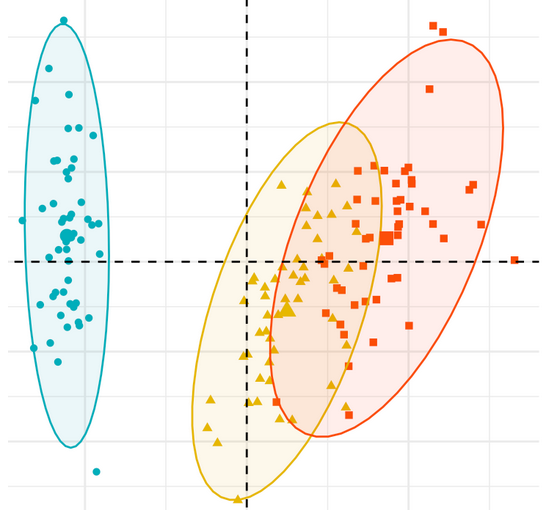
\includegraphics[height=8cm]{logos/accueil.png}
\end{center}
\vspace{10mm}

\textbf{Mémoire présenté et soutenu à Paris}

\textbf{En septembre 2021, par}

\Large {\color{Prune} \textbf{Kim ANTUNEZ}}

\vspace{15mm}

\flushleft \normalsize \textbf{Composition du jury~:}
\bigskip

\scriptsize
\arrayrulecolor{Prune}
\begin{tabular}{|p{4cm}l}
\textbf{Ivaylo Petev} &  Enseignant-chercheur en sociologie (CREST, ENSAE)\\
Directeur de mémoire & \\
\textbf{Nicolas Robette} &  Enseignant-chercheur en sociologie (CREST, ENSAE)\\
 & \\
% \textbf{} &  \\
%  & \\
% \textbf{} &  \\
%  & \\
% \textbf{} &  \\
%  & \\
% \textbf{} &  \\
%  & \\
\end{tabular}
% \begin{tabular}{p{8cm}l}
% & \\
% \textbf{} &  \\
%  & \\
% \textbf{} &  \\
%  & \\
% \textbf{} &  \\
%  & \\
% \end{tabular}

\end{titlepage}
\addamargin % this add the margin back

\frontmatter % this stuff will be roman-numbered
\pagestyle{empty} % this removes page numbers from the frontmatter



% 
  \hypersetup{linkcolor=black}
  \setcounter{secnumdepth}{2}
  \setcounter{tocdepth}{2}
  \tableofcontents




\mainmatter % here the regular arabic numbering starts
\pagestyle{fancyplain} % turns page numbering back on

\hypertarget{pruxe9face}{%
\chapter*{Préface}\label{pruxe9face}}
\addcontentsline{toc}{chapter}{Préface}

Ce mémoire de recherche a été réalisé dans le cadre de mon \textbf{double diplôme} de troisième année à l'École nationale de la statistique et de l'administration économique (\textbf{ENSAE}) et de \textbf{Master 2 de Sociologie}, parcours Sociologie Quantitative \& Démographie (SQD) accrédité Université Paris-Saclay.

J'ai souhaité, au moment du choix de mon sujet et durant la réalisation de mes travaux, allier les compétences acquises par ces deux formations. Les chercheurs en sciences sociales trouveront peut-être que la technique prend un peu trop le pas sur le raisonnement sociologique. Les statisticiens seront peut-être avides d'en savoir plus sur la théorie mathématique sur laquelle reposent les méthodes d'analyse en classes latentes. En tous cas, j'ai construit mes travaux dans l'idée de satisfaire ces deux types de profils et j'espère m'en être sortie convenablement !

Côté \textbf{sciences sociales}, j'ai fait le choix d'éclairer le phénomène de la pauvreté. Premièrement car c'était un sujet adapté à la méthodologie que je souhaitais découvrir et utiliser. Deuxièmement car le sujet était suffisamment vaste pour que je puisse découvrir la littérature sur le sujet en autodidaxie. Troisièmement car cette revue de littérature me servira probablement dans un de mes futurs postes de statisticienne publique. Quatrièmement parce que j'ai occupé dans le passé un poste de chargée d'étude sur le Baromètre d'opinion de la Drees, qui m'a procuré l'avantage de bien connaître la base de données et les thématiques qui y sont traitées.

Côté \textbf{méthodologie statistique}, le cours introductif que j'ai suivi à l'ENSAE m'a donné l'envie de creuser les méthodes à variables latentes. Introduites par les sciences humaines dès le début du XXème siècle mais très peu enseignées en France, vous verrez dans ce mémoire que ces techniques sont un complément de grande valeur aux méthodes plus classiques (économétriques et géométriques). Elles ont pour hypothèse fondamentale l'existence de variables non observables directement dans la base de données (typiquement l'intelligence, et dans notre cas la pauvreté) mais dont on peut mesurer des effets ou des conséquences. Elles sont toutefois complexes, ce qui pose parfois des difficultés de convergence des algorithmes et d'interprétation des résultats des différents modèles.

Ces travaux n'auraient pas pu voir le jour sans mon directeur de mémoire, \textbf{Ivaylo Petev}, qui a su m'encourager à me lancer dans la recherche en sciences sociales, tout en développant mon goût pour la technique en partant à la découverte des méthodes en variables latentes. Pour tout cela, je le remercie chaleureusement. Je remercie également \textbf{Nicolas Robette} pour avoir accepté d'être le second membre de mon jury et d'avoir manifesté sa curiosité concernant ces méthodes.

Enfin, j'ai voulu montrer également par ce mémoire que la \textbf{science reproductible} concerne tout autant les sciences sociales que l'informatique et la statistique. Même si je comprends les freins qui limitent parfois sa mise en œuvre (données non ouvertes, technicité des outils\ldots), je trouve qu'elle est gage de confiance puisqu'elle permet de fournir aux lecteurs l'ensemble des clefs de compréhension des résultats d'une recherche, de les critiquer (au sens noble du terme), voire de les améliorer. Même si la reproductibilité ne s'adresse pas qu'aux adaptes de la ligne de commande, elle est tout de même facilitée par certains logiciels et environnements : dans mon cas R, son arsenal \texttt{rmarkdown}, et git sans lesquels rien n'aurait non plus été possible ! Les codes et ce présent rapport sont disponibles sur \href{https://github.com/antuki/}{mon github}. Ils manquent hélas à ce jour encore un peu de tri et de documentation : les deadlines de mon année scolaire ne m'ont pas permis d'aller au bout de mes ambitions avant mes congés d'été.

Tout cela étant dit, je vous souhaite une bonne lecture !

\hypertarget{introduction}{%
\chapter*{Introduction}\label{introduction}}
\addcontentsline{toc}{chapter}{Introduction}

Il existe de nombreuses façons de définir et donc de mesurer la pauvreté. On mesure tout d'abord la pauvreté monétaire, indicateur célèbre d'inégalité mesuré notamment par les revenus, le niveau de vie, le patrimoine immobilier et financier. Il y a également en France la pauvreté institutionnelle, c'est-à-dire la relation d'assistance nouée avec l'Etat (bénéficier de prestations sociales). Il existe enfin une approche subjective de la pauvreté, selon laquelle les ménages indiquent par exemple se considérer pauvre (sentiment de pauvreté) ou craindre de le devenir, ou indiquent disposer d'un revenu inférieur au revenu minimum nécessaire pour vivre convenablement.

La considération de cette dimension subjective a permis à Duvoux \& Papuchon (2018) de mettre en exergue dans leur article de 2018 certains non-recoupements entre celle-ci et les dimensions objectives de la pauvreté traditionnellement analysées (monétaire et institutionnelle). En effet, certaines populations, bien que non pauvres monétairement, s'estiment pauvres. C'est notamment le cas de 2 \% des personnes appartenant à des ménages du dernier quintile de niveau de vie en 2019 (figure \ref{fig:figintro}, Baromètre d'opinion de la Drees). À l'inverse, certaines personnes bien qu'objectivement pauvres, ne se déclarent pas comme telles (plus de la moitié des personnes appartenant au premier quintile de niveau de vie). On parle alors d'un « halo » de la pauvreté qui illustre la difficulté, du fait de la complexité du phénomène de pauvreté, de capter uniquement par des mesures statistiques traditionnelles les personnes pauvres ou celles risquant de le devenir. Ce halo peut être approché par un certain nombre d'indicateurs de précarité, présents dans les bases de données, c'est-à-dire des facteurs de risques, étant susceptibles de faire basculer certaines populations dans la pauvreté ou de la rendre durable comme la situation par rapport au marché du travail (contrat précaire, temps partiel, chômage\ldots), le statut d'occupation du logement (locataire, logé gratuitement\ldots), ou encore certaines configurations familiales (vivre seul, familles monoparentales\ldots).
\begin{figure}[!ht]

{\centering 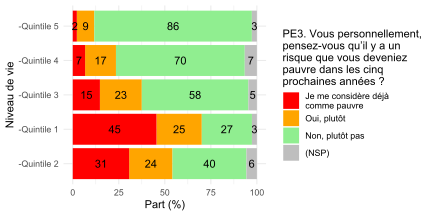
\includegraphics{M2_ANTUNEZ_SQD_files/figure-latex/figintro-1} 

}

\caption[Sentiment de pauvreté en fonction du niveau de vie en 2019]{Sentiment de pauvreté en fonction du niveau de vie en 2019}\label{fig:figintro}

\footnotesize


\emph{Source} : \emph{Baromètre d’opinion de la DREES, 2015-2019.}


\emph{Champ} : \emph{Personnes d’au moins 18 ans résidant en France métropolitaine.}
\normalsize\end{figure}

La pauvreté subjective est un autre moyen de réfléchir aux contours de ce halo de la pauvreté. Elle peut en effet apporter des informations implicites complémentaires aux mesures institutionnelle et monétaire de la pauvreté : par exemple sur les expériences antérieures de précarité des individus, ou sur la crainte de devoir (à nouveau) y faire face (insécurité sociale), en lien également avec le contexte socio-économique dans lequel ils vivent (période de crise\ldots).

Dans ce mémoire de Master 2 en sociologie quantitative, nous étudierons la nature et l'étendue du phénomène de pauvreté en France en objectivant empiriquement les contours du halo grâce aux dimensions monétaire, institutionnelle et subjective de la pauvreté identifiées dans la littérature. Nous modéliserons statistiquement les interactions entre ces différentes dimensions, en mettant en exergue des caractéristiques de la pauvreté non observées lorsque que ces dimensions sont étudiées individuellement.

Pour répondre à ces objectifs, nous mobiliserons les données du Baromètre d'opinion de la Drees. Cette enquête suit chaque année depuis 2000 l'évolution de la perception des inégalités sociales et du système de protection sociale en France. Elle permet de mesurer la plupart des dimensions de la pauvreté évoquées plus haut, objectives comme subjectives.

Après une revue de littérature dressant le contexte et la problématique de ce mémoire (chapitre \ref{chap1}), les méthodes économétriques classiques que nous mobiliserons dans un premier temps décèleront les variables expliquant le mieux la pauvreté subjective et en particulier le sentiment de pauvreté (chapitre \ref{nonreducnv}). Puis, dans un deuxième temps, nous pousserons notre analyse un peu plus loin en modélisant l'espace social de la pauvreté (chapitre \ref{esexplo}), d'abord grâce à une méthode d'Analyse des Correspondances Multiples (ACM) puis grâce à une Analyse en Facteurs communs exploratoire (AFE) qui a pour avantages de modéliser les dimensions latentes de la pauvreté et de conserver la structure des corrélations entre indicateurs. Enfin, les modèles latents confirmatoires (AFC), mis en place dans le chapitre \ref{esconfi}, montreront l'influence relative de chacune des trois dimensions sur le phénomène de pauvreté et les groupes sociaux concernés.

La vision synthétique de la pauvreté proposée prolonge les travaux de Duvoux \& Papuchon (2018) car elle quantifie et situe socialement différents pans de la pauvreté. L'identification du rôle joué par ces différents facteurs ainsi que l'analyse des populations principalement concernées, sont utiles pour décrypter les leviers sur lesquels agir pour lutter contre la pauvreté et l'exclusion sociale.

\hypertarget{chap1}{%
\chapter{Dimensions de la pauvreté : perspectives théoriques}\label{chap1}}

S'il est désormais largement reconnu que la pauvreté est multidimensionnelle, l'identification de ses différentes dimensions et de la manière dont elles interagissent ne fait pas consensus. Dans cette revue de littérature\footnote{Cette revue de littérature a été guidée et facilitée par l'excellent article de blog de Auzuret (2020)}, nous présenterons tout d'abord les différentes théories et mesures de la pauvreté (partie \ref{sec:multidim}). Puis, dans la partie \ref{sec:pauvsubj}, nous décrirons plus précisément l'approche subjective de la pauvreté, développée en particulier dans le cas de la France dans Duvoux \& Papuchon (2018). Enfin, ces différents éléments nous amèneront à exposer la démarche de ce mémoire en partie \ref{sec:objmem}, c'est-à-dire l'étude de l'interaction entre les dimensions de la pauvreté présentes dans le Baromètre d'opinion de la Drees, base de données que nous mobilisons.

\hypertarget{sec:multidim}{%
\section{La multidimensionnalité de la pauvreté soulignée dans la littérature}\label{sec:multidim}}

\hypertarget{sec:monetaire}{%
\subsection{Pauvreté monétaire}\label{sec:monetaire}}

Puisque nous vivons dans des sociétés marchandes, dans lesquelles tout bien ou service est mesuré monétairement, la question de la pauvreté est directement liée à la notion de revenus. La pauvreté est donc en premier lieu monétaire et se mesure en général au niveau du ménage, si l'on valide l'hypothèse fondamentale de mise en commun des ressources. Le repérage des ménages pauvres résulte de la comparaison de leur niveau de vie -- leur revenu disponible rapporté au nombre d'unités de consommation\footnote{Les unités de consommation sont généralement calculées selon l'échelle d'équivalence dite de l'OCDE modifiée qui attribue 1 UC au premier adulte du ménage, 0,5 UC aux autres personnes de 14 ans ou plus et 0,3 UC aux enfants de moins de 14 ans.} (UC) du ménage -- avec un seuil de pauvreté. Ce dernier est, en France et en Union Européenne en général, déterminé de manière relative (en général 50 ou 60 \% du revenu médian par UC des ménages). En 2018, en France métropolitaine, le seuil de pauvreté s'établissait pour une personne seule à 1\,063 euros par mois (Demaison, Grivet, Lesdos, \& Maury-Duprey (2020)).

Une première critique adressée à l'indicateur du seuil de pauvreté est qu'une grande partie du revenu est utilisée pour des dépenses dites « pré-engagées ». C'est d'ailleurs ce que le mouvement des « Gilets Jaunes » a permis de mettre en exergue en France durant l'hiver 2018 : même avec un emploi et des revenus relativement stables, un certain nombre de ménages ne parvenaient pas à boucler leurs fins de mois en raison de ces dépenses incompressibles, le tout dans un contexte de précarité montante (emplois à temps partiel, stagnation des salaires, inflation, en particulier des loyers, etc.). Outre les « besoins primaires » (Rawls (2020)) liés à la santé et à l'autonomie (se nourrir, se loger\ldots), doit-on prendre en considération d'autres éléments du mode de vie (voire tous) pour étudier le phénomène de la pauvreté ? C'est notamment ce que pense l'économiste et philosophe indien Amartya Sen.~Dans Sen (1985), il met l'accent sur la notion de « capacité », c'est-à-dire la liberté que doit avoir un individu de choisir entre différentes vies possibles, des souhaits qui varient selon les individus, et à un niveau plus large, selon les sociétés. Une étude de la Drees (Lelièvre \& Rémila (2018)) propose une mesure du seuil de pauvreté en déduisant des revenus les dépenses pré-engagées, et montre que les inégalités de niveau de vie sont encore plus marquées une fois que ces dépenses sont prises en compte.

Par ailleurs, la mesure relative de la pauvreté monétaire ne permet pas d'appréhender les différences de situations qui peuvent correspondre à un même niveau de vie et rend également difficile les comparaisons internationales. C'est pourquoi certaines méthodologies sont proposées afin d'étudier la pauvreté monétaire absolue -- également appelée privation matérielle -- qui correspond à un niveau de vie inférieur à la valeur d'un « panier » de biens et services dont la disposition est jugée nécessaire pour satisfaire certains besoins considérés comme essentiels. Dans l'Union européenne, une personne est réputée en situation de privation matérielle et sociale si elle déclare ne pas avoir les ressources financières suffisantes pour couvrir les dépenses liées à au moins cinq éléments de la vie courante sur treize considérés comme très souhaitables pour avoir un niveau de vie acceptable\footnote{Le dispositif européen EU‑SILC sur les revenus et les conditions de vie (Eurostat) permet d'apprécier les différences et les points communs entre pauvreté monétaire et privation matérielle et sociale.}.

Dans la même logique, l'Observatoire national de la pauvreté (Onpes) a publié des budgets de référence établis grâce à une concertation mêlant citoyens et experts. Pour chaque type de ménage (actif isolé, retraité isolé, couple d'actifs sans enfants, etc.), une liste précise de biens et de services jugés nécessaires pour participer effectivement à la vie sociale a été établie. Le montant des budgets minima de référence sont situés entre 1 424 euros et 3 284 euros, selon le type de ménage (ONPES (2015)).

\hypertarget{sec:institutionnelle}{%
\subsection{Pauvreté institutionnelle}\label{sec:institutionnelle}}

Outre la conception monétaire de la pauvreté, l'approche institutionnelle compte le nombre de ménages pauvres à partir de ceux bénéficiant des minima sociaux, c'est-à-dire d'un revenu minimum garanti basé sur des critères établis par l'État. En 2018, 11 \% de la population française était couverte par les minima sociaux, si l'on compte les conjoints et enfants à charge des bénéficiaires (Calvo (2019)).

Cette approche est inspirée de Georg Simmel et s'est développée dans un contexte du développement du chômage de masse à la suite duquel la pauvreté est devenue un objet d'intervention publique. La pauvreté institutionnelle renseigne alors sur la relation d'assistance qui lie l'individu à la société (Simmel (1998)). Selon Simmel, c'est la société qui définit en partie la pauvreté par les normes auxquelles elle se réfère pour venir en aide aux populations. Cette relation d'assistance définit la pauvreté comme une identité (Paugam \& Schnapper (1991)), plus encore qu'un état d'une personne manquant de biens matériels. Elle correspond à un statut social spécifique et dévalorisé, comme l'illustre très bien l'expression « cas sociaux » faisant référence à la fois à une situation entraînant des risques d'exclusion sociale nécessitant une prise en charge par la société mais aussi à un groupe social d'individus étant dans cette condition.

Or, cette relation d'assistance qui se noue avec l'État diffère fortement selon les cultures et les pays. Dans Esping-Andersen (1990), l'auteur décrit les processus d'émergence des trois types de régimes sociaux en Europe. Cette typologie a contribué à la considération de la protection sociale comme une dimension déterminante dans la compréhension des structures sociales des sociétés contemporaines, en lien notamment avec les politiques de luttes contre les inégalités sociales et la pauvreté. Tout d'abord, le modèle social-démocrate, le plus universaliste, accorde les mêmes droits à l'ensemble des citoyens. Le modèle libéral se fonde sur une sécurité plus minimale destinée aux personnes les plus dans le besoin. Enfin, le modèle bismarckien, auquel la France est souvent rattachée tout comme l'Allemagne, vise à maintenir un revenu en dépit des risques sociaux grâce à une assurance sociale obligatoire. Le Baromètre d'opinion de la Drees permet de voir qu'en dépit de la dominante bismarckienne du système de sécurité sociale français, les Français sont particulièrement attachés à l'universalité de certaines prestations sociales (Grislain-Letrémy \& Papuchon (2017)).

L'étude de la pauvreté ne peut donc pas se faire sans analyser en parallèle le rôle des pouvoirs publics dans la lutte contre la pauvreté. Ils peuvent en effet impulser des mesures pour augmenter les ressources des ménages (prestations sociales, baisses d'impôts\ldots) comme en France lors de la récente « Loi portant mesures d'urgence économiques et sociales » adoptée fin décembre 2018 à la suite du mouvement des « Gilets Jaunes » qui a amené notamment à revaloriser la prime d'activité. Plus anciennement, le « plan pluriannuel contre la pauvreté et pour l'inclusion sociale » de 2013 visait, en plus de réduire les inégalités, à davantage accompagner les citoyens vers l'insertion. Enfin, les pouvoirs publics insistent également beaucoup sur des politiques de reprise de l'emploi (comme le développement de l'apprentissage\footnote{Dans Cahuc, Ferracci, Tirole, \& Wasmer (2014), les auteurs montrent que, contrairement à d'autres pays, l'expansion des effectifs d'apprentis a essentiellement bénéficié aux jeunes déjà diplômés en France. Les auteurs l'expliquent par la complexité du circuit de formation professionnelle en alternance français, par la perception trop peu positive de cette orientation par le corps enseignant ou encore par la non-adéquation des formations d'apprentissage avec les besoins des entreprises.}) comme moyen de faire baisser le niveau de pauvreté. Toutefois, l'existence d'emplois de plus en plus précaires invitent à complexifier l'analyse purement monétaire de la pauvreté décrite en partie \ref{sec:monetaire}.

\hypertarget{le-halo-de-la-pauvretuxe9}{%
\subsection{Le halo de la pauvreté}\label{le-halo-de-la-pauvretuxe9}}

Les différentes dimensions et mesures de la pauvreté font souvent l'objet d'analyses sociologiques indépendantes, bien qu'elles interagissant en réalité les unes avec les autres. Le brouillage des frontières entre les différentes causes potentielles de la pauvreté est appelé « halo de la pauvreté ». Ces causes sont appelées ici « facteurs de précarité », faisant référence, comme dans Cingolani (2005) à des facteurs de risques étant susceptibles de faire basculer certaines populations plus que d'autres dans la pauvreté : temps partiels, CDD, travail intérimaire, chômage, accidents de la vie divers\ldots{}

Certaines franges de la population ont ainsi une position sociale durablement jugée inférieure sur une échelle de prestige ainsi que des difficultés à se projeter dans l'avenir : cela peut être dû à leur situation familiale (monoparentalité, famille nombreuse\ldots) ou encore aux déséquilibres du marché de l'emploi évoqué ci-dessus qui amènent à l'existence de « travailleurs pauvres » (Ponthieux (2004)). Par ailleurs, un même niveau de pauvreté n'a pas la même signification selon s'il correspond à une situation durable (ancrage dans la pauvreté) ou plus ponctuelle. C'est pourquoi il est également important d'étudier des indicateurs de dynamiques de pauvreté en plus des indicateurs d'état. Cela peut être rendu possible grâce à des analyses longitudinales de la pauvreté comme celle de Lollivier \& Verger (2005), mais celles-ci demeurent rares car les données quantitatives qui le permettent sont elles-mêmes rares.

\hypertarget{sec:pauvsubj}{%
\section{L'apport de la dimension subjective dans l'étude de la pauvreté}\label{sec:pauvsubj}}

\hypertarget{pauvretuxe9-subjective}{%
\subsection{Pauvreté subjective}\label{pauvretuxe9-subjective}}

L'approche subjective de la pauvreté s'appuie sur la manière dont les individus perçoivent leur situation. Il existe deux approches principales dans la littérature française et internationale.

La première s'intéresse aux difficultés financières perçues en mettant notamment en relation le niveau de vie minimum nécessaire -- tel qu'il ressort d'enquêtes auprès d'individus -- au niveau de vie dont ils disposent effectivement. Cette approche permet d'élaborer des seuils de pauvreté subjective (\emph{subjective poverty lines}, Veit-Wilson (1987)) et d'effectuer des comparaisons internationales sur le sujet (Paugam (2002) ; Paugam \& Selz (2005)) mais ne permet probablement pas réellement aux individus de s'affranchir des normes sociales quand ils formulent leurs réponses (Spicker, Franzoni, Leguizamón, \& Gordon (2007), p.~199).

La seconde s'intéresse à des indicateurs de privation (\emph{deprivation indicator approach}, Mack, Lansley, \& al. (1985)) telle que la mesure de la pauvreté monétaire absolue présentée plus haut qui s'intéresse à l'accès à un panier de biens et services jugés essentiels par la population.

Ces deux approches subjectives se fondent toutefois principalement sur une approche monétaire de la pauvreté qui est donc qualifiable « d'indirecte ». C'est la raison pour laquelle d'autres mesures s'intéressent également à des mesures plus « directes » de la pauvreté subjective en demandant, aux individus de s'auto-classer au niveau de la hiérarchie sociale. Toutefois, utiliser ce résultat comme mesure subjective de la pauvreté suppose que les notions de pauvreté et d'intégration sociale sont assimilables, et met de côté le lien avec l'insécurité sociale.

\hypertarget{sec:approcheduvoux}{%
\subsection{L'approche de Duvoux et Papuchon}\label{sec:approcheduvoux}}

Les travaux de Duvoux \& Papuchon (2018) confrontent les mesures monétaires et institutionnelles de la pauvreté à plusieurs mesures subjectives collectées dans le Baromètre d'opinion de la Drees. De cette manière, la pauvreté est définie de manière inductive par son aspect subjectif sans pour autant mettre de côté l'objectivation permise par les indicateurs classiques de statistique publique.

La principale mesure correspond au sentiment de pauvreté, une indicatrice des individus qui déclarent se sentir pauvre (voir la question \texttt{PE3} en annexe \ref{annexequestio}). En 2019, c'était le cas de 19 \% des Français\footnote{L'ensemble de ces chiffres, et de ceux qui suivent dans le reste du mémoire, ne concernent que les individus ayant souhaité s'exprimer (chiffres sans les « ne se prononcent pas »).}. Leur étude mobilise également, dans une moindre mesure, deux autres approches de la pauvreté subjective : une qui s'intéresse au besoin d'aide publique et une autre sur les difficultés financières perçues qui mesure l'écart entre le revenu du ménage du répondant (qu'il déclare) et celui dont un foyer comme le sien doit (selon lui) disposer au minimum pour vivre.

Ces différentes mesures de pauvreté subjective leur permettent de montrer que les mesures traditionnelles (monétaire et institutionnelle) de la pauvreté sont trop réductrices. En particulier, l'approche relationnelle d'assistance de Simmel rétrécit selon les auteurs le périmètre de la pauvreté puisque certains publics ne sont pas pris en charge par les aides sociales et que, par ailleurs, le non-recours aux prestations sociales est un sujet particulièrement présent en France. Ils cherchent donc à valider empiriquement le recours au sentiment de pauvreté en complément des indicateurs traditionnels.

En mettant en lumière le non-recoupement des définitions, ils cherchent à toucher du doigt le halo de la pauvreté évoqué plus haut. Certaines populations, bien que non pauvres monétairement, s'estiment pauvres. C'est notamment le cas de respectivement 2 \% et 7 \% des personnes appartenant à des ménages du quatrième et dernier quintile de niveau de vie en 2019 (figure \ref{fig:figintro}). À l'inverse, certaines personnes, bien qu'objectivement pauvres, ne se déclarent pas comme telles (plus de la moitié des personnes appartenant au premier quintile de niveau de vie). Ils apportent une illustration à la thèse selon laquelle le sentiment de pauvreté ne concerne pas que les personnes en situation d'assistance ou éloignées du marché du travail mais concerne également une partie des personnes en emploi, notamment les ouvriers et les employés.

Enfin, ils insistent sur l'appréciation négative portée par les personnes qui se déclarent pauvres sur leur trajectoire passée et leur avenir et en concluent que « la pauvreté subjective se comprend sociologiquement comme un indicateur d'insécurité sociale durable ». Ce point précis a fait l'objet de quelques controverses sociologiques exposées dans la partie \ref{sec:limitesduvoux} qui suit.

\hypertarget{sec:limitesduvoux}{%
\subsection{Les limites identifiées d'une telle approche}\label{sec:limitesduvoux}}

Cet article a été l'origine de deux discussions (Paugam (2020) et Lahieyte (2020)) permettant de revenir sur l'approche proposée par les précédents auteurs.

Les débats portent tout d'abord sur les éventuels biais dans la mesure du sentiment de pauvreté. Comme dans toute enquête, d'autant plus s'agissant d'une enquête d'opinion, les réponses sont liées à la formulation de la question. Or, la question utilisée semble imprécise selon plusieurs aspects, ce qui rend difficile l'identification de ce qui est réellement mesuré. On ne sait pas ce que les enquêtés entendent par « un foyer comme le leur » et font-ils bien dans leurs réponses référence au revenu de leur ménage ou bien uniquement au leur ? Les réponses dépendent également du rapport qui se tisse entre enquêteur et enquêté : il est fort probable que certaines personnes pourraient ne pas oser se déclarer pauvres. D'ailleurs, le fort pourcentage de non-réponse à cette question (6 \% en 2019 contre un maximum de 1 ou 2 pourcents pour la plupart des questions de l'enquête) va dans le sens de cette interprétation. C'est pourquoi Duvoux \& Papuchon (2020) recommandent dans leur réponse de s'intéresser davantage à l'interprétation des résultats en gardant en tête le fait que cet indicateur est un proxy permettant de mesurer tout un ensemble d'éléments complexes à appréhender, comme dans toute enquête d'opinion.

D'après Paugam (2020), les auteurs opposent également trop souvent l'aspect subjectif (pauvreté déclarée) à l'aspect institutionnel (perception de minima sociaux) et devraient davantage faire le lien entre les deux. Selon Paugam, le sentiment d'être pauvre serait prioritairement mis en lien par les auteurs avec le climat d'insécurité sociale qui accompagne la crise salariale et pas assez avec la prise en charge institutionnelle de l'assistance montrée par Simmel. Pourtant, toujours selon Paugam, le développement de l'assistance est, depuis les années 1980, en France et dans les pays occidentaux, une conséquence directe de la précarisation des emplois et de la montée du chômage.

De manière générale, Duvoux et Papuchon partent de l'hypothèse que leur mesure du sentiment de pauvreté traduit avant tout une condition d'insécurité sociale, c'est-à-dire de déficit de garantie face à l'avenir. Or, ils n'insistent pas assez, selon Paugam, sur une autre interprétation qu'il juge plus importante : l'infériorité sociale, c'est-à-dire le manque de reconnaissance sociale et le sentiment d'inutilité sociale. Ces différents éléments d'explication peuvent d'ailleurs être en partie testées grâce aux données des modules thématiques de questions « opinion générale » et « pauvreté / exclusion » du Baromètre de la Drees. Concernant l'insécurité sociale, on interroge notamment les Français sur leur optimisme face à l'avenir (pour eux, mais aussi pour les générations futures) et sur leur vision sur l'évolution passée et à venir des inégalités d'une part et de la pauvreté et l'exclusion d'autre part. Pour l'infériorité sociale, l'appréciation des Français sur la manière (de très mauvaise à très bonne) dont ils considèrent leur situation actuelle ou sur leur sentiment ou non d'avoir une situation moins bonne que leurs parents au même âge (déclassement intergénérationnel) pourrait éclairer une partie du phénomène.

\hypertarget{sec:objmem}{%
\section{Etudier les interactions entre les dimensions de la pauvreté}\label{sec:objmem}}

\hypertarget{objectif-moduxe9liser-lespace-social-de-la-pauvretuxe9}{%
\subsection{Objectif : modéliser l'espace social de la pauvreté}\label{objectif-moduxe9liser-lespace-social-de-la-pauvretuxe9}}

La pauvreté, en plus d'être multidimensionnelle et de reposer sur des dimensions qui ne se recoupent pas entièrement, dépend donc aussi de situations individuelles particulières et de facteurs potentiellement inobservables. Cela explique la difficulté méthodologique de définir ce phénomène. Quand bien même on arriverait à définir les indicateurs les plus pertinents, il faudrait ensuite définir un moyen de construire une échelle de la pauvreté. Or, dès lors que l'on sort du cadre de l'unidimensionnalité, on ne dispose pas d'une méthode exacte pour classer sans ambiguïté les individus dans des « catégories de pauvreté ». Et peut-on vraiment considérer la pauvreté comme étant ordinale quand on se base sur les théories de liberté de choix individuels et de pluralisme des goûts comme le fait Sen (1985) ?

Cette complexité du sujet même de pauvreté et les débats sur la détermination de ses dimensions a fait naître des initiatives internationales de recherche participative sur les dimensions de la pauvreté comme celle de l'association Monde (2019). Des personnes en situation de pauvreté, des professionnels et des universitaires de différents pays\footnote{Au Bangladesh, en Bolivie, en France, en Tanzanie, au Royaume-Uni et aux États-Unis.} ont travaillé ensemble pour aboutir à trois groupes de dimensions de la pauvreté (figure \ref{fig:figatd}) interdépendantes faisant la synthèse de ce qui a été évoqué précédemment. Le premier groupe, situé au centre de la figure \ref{fig:figatd}, forme le cœur de l'expérience de la pauvreté : les souffrances physiques ou mentales résultant de la dépossession du pouvoir d'agir (le manque de contrôle sur sa vie), causées par les privations auxquelles les personnes réagissent par de la lutte et de la résistance. Un deuxième groupe rassemble les dimensions relationnelles de la pauvreté : les maltraitances institutionnelles (incapacité des institutions à répondre aux besoins), sociales (par d'autres groupes sociaux) et les compétences non reconnues des personnes en situation de pauvreté. Le dernier groupe rassemble les privations : le manque de travail décent, le revenu insuffisant et les privations matérielles et sociales. Les neuf dimensions évoquées, et donc l'intensité de la pauvreté, peuvent être modifiées par cinq facteurs : l'identité (genre, appartenance ethnique, etc.), le temps (le moment de la vie où elle est vécue), le lieu (pays mais aussi urbain versus rural), l'environnement (météo, inondations, sècheresse\ldots) ainsi que les croyances culturelles : la société en elle-même impulse des dépenses obligatoires dans le cadre de traditions qui jouent sur les revenus (la dot, les cadeaux\ldots).
\begin{figure}[!ht]

{\centering 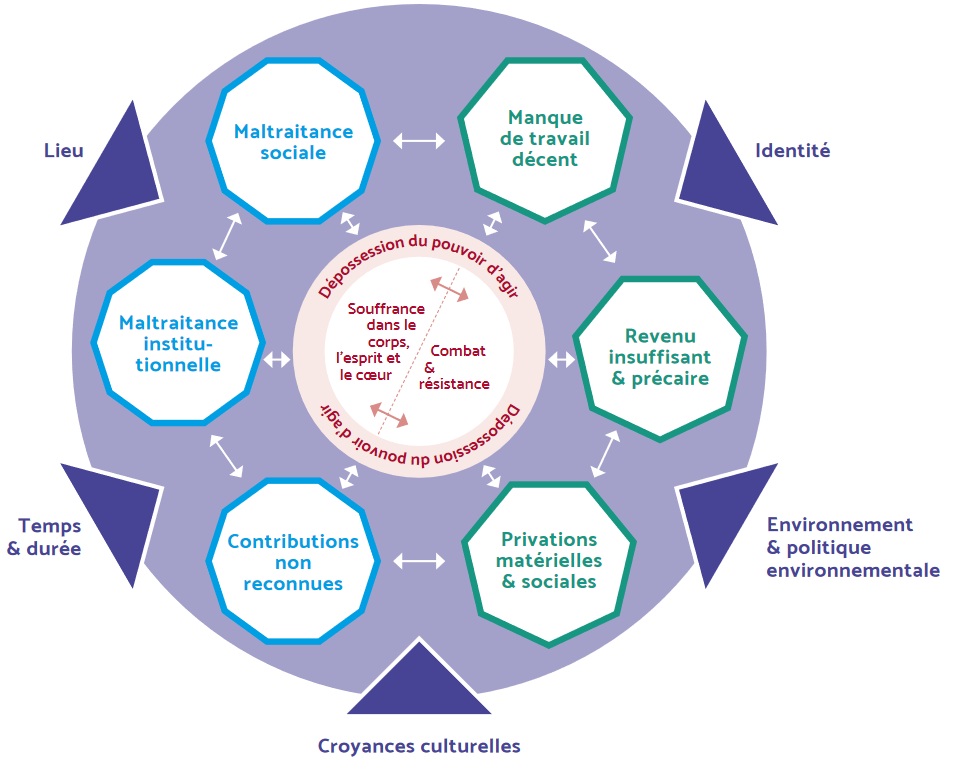
\includegraphics[width=0.8\linewidth]{figures/fig_atd} 

}

\caption[Graphique sur les dimensions de la pauvreté]{Graphique sur les dimensions de la pauvreté}\label{fig:figatd}

\footnotesize


\emph{Source} : \emph{ATD Quart Monde et Université d’Oxford, janvier 2019}
\normalsize\end{figure}

Dans le cadre de ce mémoire de Master 2 en sociologie quantitative, nous avons cherché à reconstruire empiriquement l'espace social de la pauvreté. Pour cela, nous avons mobilisé les données du Baromètre d'opinion de la Drees, comme Duvoux \& Papuchon (2018). Cette base de données comporte des mesures des principales dimensions de la pauvreté identifiées dans la revue de littérature du chapitre \ref{chap1} à savoir monétaire, institutionnelle et subjective. Toutefois, étant un baromètre d'opinion elle a le désavantage de ne pas être particulièrement fournie en indicateurs objectifs.

Nous répondons à cet objectif grâce à des méthodes économétriques robustes, faisant notamment intervenir des analyses en variables latentes. Cette modélisation synthétique du phénomène de pauvreté permet d'analyser le positionnement des dimensions subjective et institutionnelle de la pauvreté par rapport à la dimension monétaire et de situer socialement le rôle de chacune de ces dimensions.

\hypertarget{base-de-donnuxe9es-le-baromuxe8tre-dopinion-de-la-drees}{%
\subsection{Base de données : Le Baromètre d'opinion de la Drees}\label{base-de-donnuxe9es-le-baromuxe8tre-dopinion-de-la-drees}}

\hypertarget{un-outil-de-suivi-conjoncturel-depuis-2000}{%
\subsubsection{Un outil de suivi conjoncturel depuis 2000}\label{un-outil-de-suivi-conjoncturel-depuis-2000}}

Le Baromètre d'opinion de la DREES\footnote{La présentation du Baromètre faite ici est très fortement inspirée de celle proposée par la Drees dans ses publications.} recense chaque année depuis 2000 l'évolution de l'opinion des Français sur leur santé, sur la protection sociale dans l'ensemble de ses dimensions (assurance maladie, retraite, famille, handicap, dépendance, solidarité, lutte contre la pauvreté et l'exclusion) ainsi que sur les inégalités et la cohésion sociale (depuis 2014).

À la demande de la Drees (Service statistique du ministère des Solidarités et de la Santé), l'institut BVA réalise cette enquête en face-à-face auprès d'un échantillon de 3 000 personnes différentes chaque année, représentatif de la population habitant en France métropolitaine âgée de 18 ans et plus. Cet échantillon est construit selon la méthode des quotas, par sexe, âge, profession de la personne de référence, après stratification par région et catégorie d'agglomération.

Le caractère annuel et l'ancienneté de ce baromètre en font un outil de suivi conjoncturel de référence indispensable pour appréhender l'évolution de l'opinion des Français sur les politiques dont le ministère des Solidarités et de la Santé a la charge, tant en matière de santé que de solidarité. Le Baromètre apporte un éclairage complémentaire aux travaux menés habituellement par la Drees, puisqu'il permet de mettre en parallèle les évolutions perçues et réelles des politiques sanitaires et sociales. Il est notamment régulièrement utilisé à ce titre par des chercheurs en sociologie et en science politique.

\hypertarget{appruxe9hender-lopinion-sur-dix-thuxe9matiques}{%
\subsubsection{Appréhender l'opinion sur dix thématiques}\label{appruxe9hender-lopinion-sur-dix-thuxe9matiques}}

Le questionnaire vise à connaître les attentes et les préoccupations des Français sur le fonctionnement du système actuel et sur de potentielles réformes. Il s'articule autour de plusieurs modules thématiques cités ci-dessous. Les thèmes suivis d'un astérisque (*) sont davantage approfondis en années paires, grâce à la présence de questions supplémentaires bisannuelles. À l'inverse, les thèmes non suivis d'un astérisque sont approfondis en années impaires.
\begin{itemize}
\tightlist
\item
  Inégalités* (inégalités de revenus, inégalités entre femmes et hommes, justice sociale, etc.) ;
\item
  Pauvreté et exclusion* (évolution de la pauvreté, définition des personnes exclues, opinion sur le montant et l'efficacité du RSA et des allocations chômage, etc.) ;
\item
  Protection sociale (financement de la protection sociale, ciblage des prestations sur les plus modestes ou les seuls cotisants, etc.) ;
\item
  Retraites (âge de départ anticipé et souhaité, niveau de vie des retraités, réformes souhaitées pour préserver le système de retraite, etc.) ;
\item
  Santé (perception de l'état de santé de la population, qualité et accès aux soins, risque sanitaire, inégalités de santé, réformes souhaitées, etc.) ;
\item
  Famille* (objectif que doit poursuivre la politique familiale, durée du congé maternité, mode de garde privilégié pour les enfants en bas âge, etc.) ;
\item
  Handicap (effort de la société envers les personnes handicapées, etc.) ;
\item
  Dépendance (création d'une cotisation obligatoire pour aider financièrement les personnes dépendantes, statut des aidants, etc.) ;
\item
  Logement (difficulté pour se loger, etc.) ;
\item
  Cohésion sociale* (sentiment d'intégration, laïcité, discriminations, non-recours, etc.).
\end{itemize}
\hypertarget{pruxe9cautions-dinterpruxe9tation-des-enquuxeates-dopinion}{%
\subsubsection{Précautions d'interprétation des enquêtes d'opinion}\label{pruxe9cautions-dinterpruxe9tation-des-enquuxeates-dopinion}}

Les réponses à une enquête d'opinion sont particulièrement sensibles à la formulation des questions et à leur place dans le questionnaire. Du fait de l'ancienneté et de la stabilité du questionnaire du Baromètre, ses différentes éditions permettent néanmoins des comparaisons entre catégories (selon le revenu, l'âge, etc.) et dans le temps. Toutefois, compte tenu de la taille de l'échantillon, de faibles variations peuvent ne refléter que des imperfections de mesure.

\hypertarget{accuxe9der-aux-donnuxe9es}{%
\subsubsection{Accéder aux données}\label{accuxe9der-aux-donnuxe9es}}

Les bases contenant l'intégralité des données individuelles du Baromètre d'opinion de la Drees sont en libre accès depuis 2019. Elles sont mises en ligne sur sa \href{http://www.data.drees.sante.gouv.fr/}{plateforme de diffusion de données} . Elles sont accompagnées de fichiers Excel présentant les résultats pour chaque question en historique (tris à plat) et les résultats croisés avec les principales variables sociodémographiques pour la dernière année disponible (tris croisés). Un \href{http://dataviz.drees.solidarites-sante.gouv.fr/Barometre-DREES}{outil de visualisation interactive} permet de visualiser et télécharger sous forme de tableaux et graphiques l'ensemble des résultats du Baromètre d'opinion de la DREES depuis 2000. Plus d'informations sont disponibles sur la \href{https://drees.solidarites-sante.gouv.fr/etudes-et-statistiques/open-data/aide-et-action-sociale/article/le-barometre-d-opinion-de-la-drees}{page internet de la DREES dédiée au Baromètre}.

\hypertarget{sec:methodo}{%
\subsection{Méthodologie}\label{sec:methodo}}

\hypertarget{sec:mesures}{%
\subsubsection{Stratégie empirique et mesures}\label{sec:mesures}}

Dans cette étude, nous compilons les réponses obtenues lors des cinq dernières vagues d'enquêtes (2015 à 2019) pour avoir des effectifs suffisants (plus de 15 000 répondants), ceci afin d'obtenir des résultats significatifs, sans pour autant mobiliser des données trop anciennes. Les données ont été collectées avant la crise sanitaire du Covid-19, ce qui permet de ne pas faire intervenir un certain nombre de facteurs d'incertitudes liés à cette crise dans notre analyse. Il est à noter que le Baromètre \textbf{n'est pas un panel} et que sont interrogées chaque année des personnes différentes.

Les variables de l'enquête plus particulièrement mobilisées pour cette étude sont décrites ci-dessous. Elles ont permis d'opérationnaliser les différentes dimensions de la pauvreté : monétaire, institutionnelle, et subjective, ainsi que différentes variables de contrôles sociodémographiques, parfois facteurs de précarité. Les \texttt{codes} des questions font référence à ceux tels qu'ils sont référencés dans le questionnaire du Baromètre dont un extrait est reproduit en annexe \ref{annexequestio}.

Dans le Baromètre d'opinion, les enquêtés sont interrogés sur les types de revenus perçus par \textbf{leur ménage} (\texttt{SDRES}), à la fois des revenus issus de salaires, pensions ou de placement financiers (dimension monétaire\footnote{Salaires, traitements et primes / Revenus d'une activité professionnelle indépendante / Préretraite, retraites / Revenus d'actifs financiers / Revenus de locations.}) mais également différentes prestations sociales (dimension institutionnelle\footnote{RSA (Revenu de solidarité active) / Allocations de chômage / Prestations familiales (allocations familiales, complément familial, prestation d'accueil du jeune enfant {[}PAJE{]}\ldots) / Allocations de logement (APL, \ldots) / Prestations liées au handicap, à l'invalidité ou à la dépendance (AAH, APA, PCH\ldots) / Bourses d'études.}) ainsi que des pensions alimentaires éventuelles (non utilisées dans ce mémoire).

Ils sont également questionnés sur le revenu mensuel net de leur ménage avant impôt (\texttt{SDREVCL}) tenant compte de tous les types de revenus perçus par le ménage listés dans le paragraphe précédent. S'ils ne répondent pas à cette question, on leur propose de renseigner une tranche de revenus (\texttt{SDREVTR}) afin de réduire au maximum la non-réponse. Malgré ces précautions, la question des revenus reste la question avec le plus fort taux de non-réponse (7 \% sur 2015 à 2019 sur le revenu en tranches et 23 \% sur le montant précis). En cas de non-réponse, nous imputons donc le montant précis en attribuant au ménage ayant uniquement répondu à la partie en tranche la moyenne déclarée dans la variable « montants » pour les enquêtés se situant dans la même tranche (imputation par les moyennes conditionnelles). Puis, nous rapportons ce montant au nombre d'unités de consommation du ménage afin de calculer le niveau de vie\footnote{Le niveau de vie se mesure au niveau du ménage. Il est égal au revenu disponible du ménage divisé par le nombre d'unités de consommation (UC).}.

\textbf{Pauvreté subjective}

Le Baromètre d'opinion a pour particularité de collecter des indicateurs subjectifs, en particulier de pauvreté. Nous nous concentrons sur deux indicateurs intéressants pour ce mémoire : le sentiment de pauvreté et les difficultés financières perçues.

Le sentiment de pauvreté s'appréhende par la proportion de Français qui, à la question \texttt{PE3} « Et vous personnellement, pensez-vous qu'il y a un risque que vous deveniez pauvre dans les cinq prochaines années ? », répondent « Je me considère déjà comme pauvre ». La modalité intermédiaire « Oui, plutôt » est également mobilisée dans les analyses factorielles et en facteurs communs du chapitre \ref{esexplo} ainsi que dans le chapitre \ref{esconfi}.

Par difficultés financières perçues, nous entendons le fait d'indiquer avoir dans son foyer des revenus inférieurs à ce que l'on considère comme étant le minimum pour vivre. Il s'agit de la situation pour laquelle la réponse à la question \texttt{PE16} « Selon vous, pour vivre, quel est le montant dont doit disposer AU MINIMUM un foyer comme le vôtre, par mois (en euros) ? » est inférieure à celle de la question \texttt{SDREVCL} « Nous désirons savoir à quel niveau de revenus MENSUELS NETS AVANT IMPOTS se situe votre foyer » dont on a imputé de la non-réponse par moyennes conditionnelles.

\textbf{Variables de contrôle sociodémographiques}

Différentes variables sociodémographiques sont également mobilisées tout au long de ce mémoire de manière à situer socialement les différentes interactions entre les dimensions de la pauvreté. Il s'agit principalement du sexe (\texttt{SDSEXE}), de la tranche d'âge (à partir de \texttt{SDAGE}), de la situation sur le marché du travail (principalement \texttt{SDPCS10}), de la situation familiale (\texttt{SDSITFAM}), du statut d'occupation du logement (\texttt{LO1}) et du niveau de diplôme (\texttt{SDDIPL}).

\hypertarget{sec:methodes}{%
\subsubsection{Méthodes statistiques utilisées}\label{sec:methodes}}

Dans le chapitre \ref{chap1}, nous utilisons des modèles de régression logistique où les deux indicateurs de pauvreté subjective constituent les variables dépendantes afin d'expliquer leurs déterminants.

Dans le chapitre \ref{esexplo}, nous mobilisons deux méthodes de représentation visuelle de l'espace social de la pauvreté à partir de mesures issues des trois dimensions de la pauvreté : monétaire, institutionnelle et subjective. La première méthode, rendue particulièrement célèbre par les travaux de Pierre Bourdieu en France, est une Analyse des Correspondances Multiples (ACM) suivie d'une Classification Ascendante Hiérarchique (CAH) afin de regrouper en classes les individus qui se ressemblent selon les différents indicateurs de pauvreté. La seconde méthode est une Analyse en Facteurs communs Exploratoire (AFE). Même si on l'assimile souvent à des méthodes type ACM, ces deux notions sont pourtant très différentes : l'ACM correspond à un modèle descriptif des données alors que l'AFE est un modèle structurel. Cette dernière méthode possède l'outillage mathématique permettant de modéliser des dimensions latentes qui se cachent derrière les variables mesurées, en conservant la structure des corrélations entre ces dernières (voir les détails techniques en annexe \ref{sec:annexeAFAFE}).

Dans le chapitre \ref{esconfi}, des modèles d'Analyse en Facteurs communs Confirmatoires (AFC) sont mis en place (détails en annexe \ref{sec:annexeAFAFC}). Alors que l'AFE permet de déterminer les facteurs latents et de détecter les indicateurs notoires qui les définissent, l'AFC permet de tester empiriquement des hypothèses de structures factorielles à partir d'hypothèses structurales formulées dans la littérature. Les modèles d'AFC permettent ainsi de mesurer l'influence relative de chacune des trois dimensions sur le phénomène de pauvreté et d'également situer chacune d'elle socialement.

\hypertarget{nonreducnv}{%
\chapter{Le sentiment de pauvreté ne se réduit pas au niveau de vie}\label{nonreducnv}}

Dans ce deuxième chapitre, nous analysons les déterminants de deux indicateurs de pauvreté subjective collectés dans le Baromètre d'opinion de la Drees : le sentiment de pauvreté (indiquer se sentir pauvre) et les difficultés financières perçues (indiquer avoir dans son foyer des revenus inférieurs à ce que l'on considère comme étant le minimum pour vivre).

Nous verrons que même si le niveau de vie explique fortement ces indicateurs de pauvreté subjective, les indicateurs de pauvreté monétaire ne suffisent pas à eux-seuls. Ce résultat sera d'ailleurs introduit par un paradoxe : alors que les indicateurs de pauvreté subjective se sont détériorés depuis 2015 -- en particulier à partir de 2018 -- la pauvreté monétaire est, elle, restée stable voire a diminué. Cela montre alors l'intérêt de s'intéresser à une autre dimension de la pauvreté dont nous disposons dans le Baromètre : la pauvreté institutionnelle (bénéficier de certaines prestations sociales au niveau de son ménage).

Outre les indicateurs des différentes dimensions de la pauvreté, nous verrons que d'autres caractéristiques influent sur le fait de se sentir pauvre : ne pas être propriétaire de son logement, être en dehors du marché du travail ou, dans une moindre mesure, être ouvrier ou employé, vivre seul ou encore être à la tête d'une famille monoparentale.

\hypertarget{sec:augmentesubj}{%
\section{À partir de 2018, le sentiment de pauvreté augmente mais ses facteurs explicatifs ne sont pas radicalement modifiés}\label{sec:augmentesubj}}

Le Baromètre d'opinion de la Drees permet de mesurer le niveau et l'évolution au cours du temps du sentiment de pauvreté\footnote{Pour rappel, le sentiment de pauvreté s'appréhende dans le Baromètre d'opinion par la proportion de Français qui, à la question \texttt{PE3} « Et vous personnellement, pensez-vous qu'il y a un risque que vous deveniez pauvre dans les cinq prochaines années ? », répondent « Je me considère déjà comme pauvre » (voir extrait de questionnaire en annexe \ref{annexequestio}).} des Français. Celui-ci a sensiblement augmenté ces dernières années, en particulier depuis 2018, pour atteindre 19 \% en 2019 (figure \ref{fig:figchap1compa20152019}). Il en va de même pour les difficultés financières qui sont ressenties\footnote{Quand la réponse à la question \texttt{PE16} « Selon vous, pour vivre, quel est le montant dont doit disposer AU MINIMUM un foyer comme le vôtre, par mois (en euros) ? » est inférieure à celle de la question \texttt{SDREVCL} « Nous désirons savoir à quel niveau de revenus MENSUELS NETS AVANT IMPOTS se situe votre foyer » dont on a imputé de la non-réponse (voir partie \ref{sec:mesures}).} par plus de la moitié des Français, et ce depuis les cinq dernières années.
\begin{figure}[!ht]

{\centering 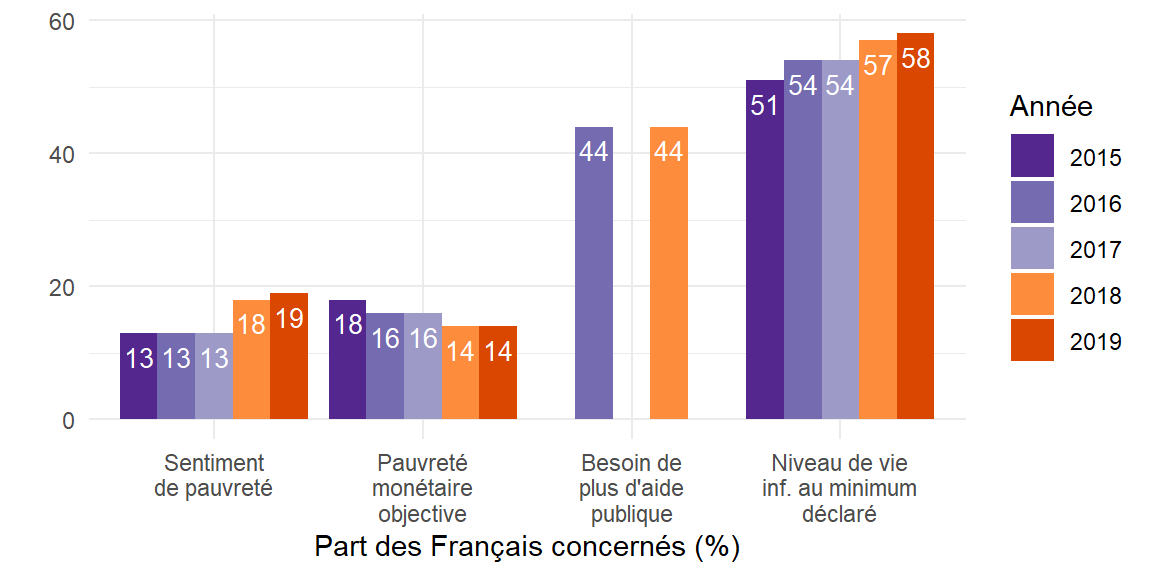
\includegraphics{M2_ANTUNEZ_SQD_files/figure-latex/figchap1compa20152019-1} 

}

\caption[Différents indicateurs de pauvreté (2015 à 2019)]{Différents indicateurs de pauvreté (2015 à 2019)}\label{fig:figchap1compa20152019}

\footnotesize


\emph{Source} : \emph{Baromètre d’opinion de la DREES, 2015-2019.}


\emph{Champ} : \emph{Personnes d’au moins 18 ans résidant en France métropolitaine.}


\emph{Note} : \emph{Les barres noires correspondent aux intervalles de confiance à 95 \%. La borne d'erreur a été calculée avec la formule : $({z}_{\frac{{\alpha}}{{2}}})(\sqrt{\frac{{p'(1-p')}}{{n}}}$ avec $p' = \frac{x}{n}$ la proportion estimée de réponses affirmatives à la question ($x$ étant le nombre de réponses affirmatives et $n$ la taille de l'échantillon). Pour plus de détails concernant le calcul voir \href{https://courses.lumenlearning.com/atd-odessa-statistics/chapter/a-population-proportion/}{ici}. Grossièrement, on peut considérer que si l’on prend l’ensemble de l’échantillon d’un même millésime d’enquête (3 000 répondants), une évolution est significative si elle est supérieure au seuil de 4 points de pourcentage. Ce seuil est supérieur quand les effectifs sont plus petits : par exemple quand les valeurs manquantes sont nombreuses (typiquement pour le niveau de vie) ou lorsque l’on travaille sur des sous-populations.}
\normalsize\end{figure}

En parallèle, la pauvreté objective -- qui correspond à la proportion de Français en dessous du seuil de pauvreté (seuil de 60 \% du revenu médian\footnote{Cet indicateur ne correspond pas aux données nationales officielles mais à un calcul avec les données du Baromètre. La source qui fait référence en France pour le taux de pauvreté (Insee, ERFS) donne, elle, des taux en légère augmentation depuis 2015 : 14,3 \% pour 2015, 13,9 \% pour 2016, 14,1 \% pour 2017 et 14,8 \% pour 2018.}) stagne voire diminue légèrement et atteint 14 \% en 2019. Enfin, 44 \% des Français jugent en 2019 ne pas être suffisamment aidés par les pouvoirs publics\footnote{Réponse « Vous auriez besoin d'être aidé(e) davantage par les pouvoir publics » à la question \texttt{PE15} : « Actuellement, compte tenu de votre situation globale, du montant des aides publiques (RSA, allocations familiales, aides au logement), et du montant de vos impôts, vous considérez que\ldots{} ». Cette question est posée uniquement en \textbf{années paires}, c'est pourquoi nous ne l'avons pas utilisée dans le reste de ce mémoire.}.

Cette décorrélation de l'évolution globale des pauvretés subjective et monétaire s'illustre également dans les données récentes du Baromètre, collectées à la fin de l'année 2020 et ayant fait l'objet d'une publication en juillet 2021 (Lardeux, Papuchon, \& Pirus (2021)). Fin 2020\footnote{La collecte du Baromètre a lieu chaque année entre octobre et décembre.}, un quart des Français indiquent que leur situation financière s'est détériorée depuis la crise de la Covid-19. Pour autant, l'année 2020 n'est pas marquée par une augmentation du sentiment de pauvreté, à l'exception de chez les plus jeunes.

L'année 2018 marque donc un tournant particulièrement fort dans l'évolution du sentiment de pauvreté. Cette hausse s'accompagne d'une sensibilité accrue aux inégalités de revenus puisque ce type d'inégalité est cité en 2018 par 22 \% des Français (+7 points par rapport à 2017) comme étant la moins acceptable, un niveau supérieur à celui des inégalités de santé, alors que ça n'avait jamais été le cas jusqu'à présent (Antunez \& Papuchon (2019)). La fin de l'année 2018 correspond également à la naissance du mouvement social français des « Gilets jaunes » revendiquant l'amélioration du niveau de vie des classes populaires et moyennes. L'intégration de ces dernières vagues d'enquête (2018 et 2019) présente alors un intérêt tout particulier.

Si l'on s'intéresse au niveau et à l'évolution du sentiment de pauvreté selon différentes caractéristiques des répondants, certaines disparités sociales se dessinent très clairement. Notamment, la moitié des Français n'exerçant aucune activité professionnelle, y compris ceux étant à la recherche d'un emploi, indiquent se sentir pauvre (figure \ref{fig:figstatactevol}). Depuis 2018, l'écart avec les actifs, étudiants et retraités s'est même très fortement creusé. Cette exposition forte au sentiment de pauvreté conforte les théories de Castel (Castel \& Beland (2004) et Castel (2014)) selon lesquelles les populations exclues du marché du travail auraient un risque accru et croissant d'insécurité sociale\footnote{Mais le sentiment de pauvreté révèle-t-il principalement un sentiment d'insécurité sociale ? Pas nécessairement ! On a vu en partie \ref{sec:limitesduvoux} que Paugam (2020) insiste également sur le rôle de la charge institutionnelle de l'assistance sur le fait de se sentir pauvre.} (revenus instables rendant difficile la projection vers l'avenir).
\begin{figure}[!ht]

{\centering 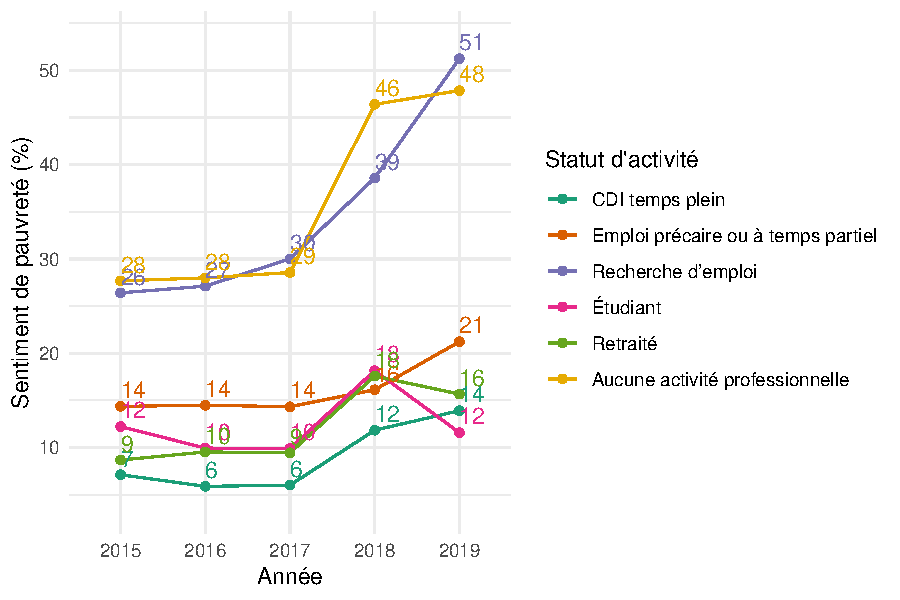
\includegraphics{M2_ANTUNEZ_SQD_files/figure-latex/figstatactevol-1} 

}

\caption[Evolution du sentiment de pauvreté selon le statut d'activité]{Evolution du sentiment de pauvreté selon le statut d'activité}\label{fig:figstatactevol}

\footnotesize


\emph{Source} : \emph{Baromètre d’opinion de la DREES, 2015-2019.}


\emph{Champ} : \emph{Personnes d’au moins 18 ans résidant en France métropolitaine.}
\normalsize\end{figure}

Des disparités s'observent également par catégorie professionnelle. Près d'une personne n'ayant jamais travaillé sur trois, d'un ouvrier ou ancien ouvrier sur trois et d'un employé ou ancien employé sur cinq se déclarent pauvre en 2019 (figure \ref{fig:figstatactevol}). Là encore, les écarts avec les autres professions se creusent dans le temps, en particulier depuis 2018\footnote{Pour les agriculteurs, la tendance du sentiment de pauvreté est également à la hausse mais correspond à un plus effectif de répondants trop faible pour être analysé.}.
\begin{figure}[!ht]

{\centering 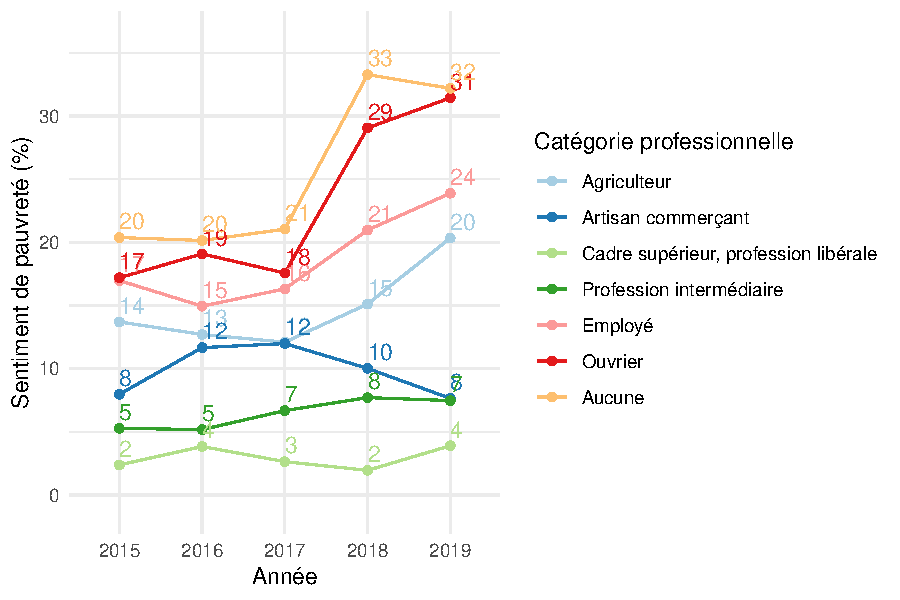
\includegraphics{M2_ANTUNEZ_SQD_files/figure-latex/figpcsevol-1} 

}

\caption[Evolution du sentiment de pauvreté selon la catégorie professionnelle]{Evolution du sentiment de pauvreté selon la catégorie professionnelle}\label{fig:figpcsevol}

\footnotesize


\emph{Source} : \emph{Baromètre d’opinion de la DREES, 2015-2019.}


\emph{Champ} : \emph{Personnes d’au moins 18 ans résidant en France métropolitaine.}
\normalsize\end{figure}

Enfin, tous les types de ménages ne sont pas exposés de la même manière au sentiment de pauvreté (figure \ref{fig:figviefamevol}). En premier lieu, les femmes cheffes de familles monoparentales sont concernées pour un tiers d'entre elles. La fragilité financière des familles monoparentales est traitée dans la littérature depuis plusieurs dizaines d'années, notamment dans le cas français avec ce bref article de Wright (1991) qui montre que les familles monoparentales, en particulier celles avec une femme à leur tête, étaient surreprésentées dans les rangs de la pauvreté en 1979. Plus récemment, Argouarc'h \& Boiron (2016) indiquent qu'en 2014 le taux de pauvreté des familles monoparentales s'élevait à 35,9 \%, soit plus de 20 points au-dessus de la moyenne de l'ensemble des familles.
\begin{figure}[!ht]

{\centering 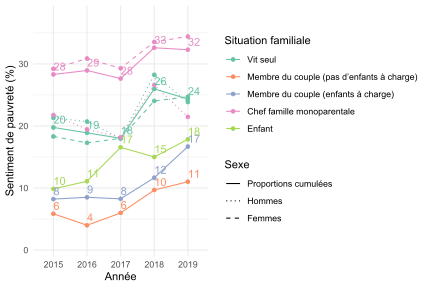
\includegraphics{M2_ANTUNEZ_SQD_files/figure-latex/figviefamevol-1} 

}

\caption[Evolution du sentiment de pauvreté selon la situation familiale]{Evolution du sentiment de pauvreté selon la situation familiale}\label{fig:figviefamevol}

\footnotesize


\emph{Source} : \emph{Baromètre d’opinion de la DREES, 2015-2019.}


\emph{Champ} : \emph{Personnes d’au moins 18 ans résidant en France métropolitaine.}


\emph{Note} : \emph{Les effectifs des hommes chefs de famille monoparentale sont trop faibles pour être interprétés.}
\normalsize\end{figure}

Une personne vivant seule sur cinq se sent également pauvre ; c'est la situation familiale pour laquelle le sentiment de pauvreté a le plus augmenté depuis 2015, là encore en particulier depuis 2018. À l'inverse, seul un couple avec enfant sur dix se déclare pauvre. Ces résultats semblent illustrer le rôle protecteur de la famille (conjoint et enfants) vis-à-vis de la pauvreté. Être en couple permet de faire au quotidien des économies d'échelles et augmente également les chances de percevoir un salaire au sein du ménage, en particulier pour les femmes (Dauphin \& Domingo (2014)). L'entourage familial limite également potentiellement le sentiment d'insécurité sociale. Réciproquement, avoir des enfants peut être conçu comme étant une richesse pour les familles pauvres attachées aux valeurs familiales ; et le cercle familial apporte alors sécurité, ancrage identitaire et social (Paugam (2005)). Pour d'autres, le sentiment de pauvreté peut aussi limiter le souhait d'avoir un enfant par crainte de ne pas être en mesure de subvenir correctement à ses besoins.

Pour expliquer les déterminants du sentiment de pauvreté au-delà de ces premières statistiques descriptives, un premier modèle de régression logistique où le fait de se déclarer pauvre constitue la variable dépendante est utilisé. Il s'agit d'une reproduction de résultats provenant de Duvoux \& Papuchon (2018) construits à partir de la base 2015--2017 (avant dernière colonne) ainsi qu'une réplication de ceux-ci intégrant en plus les millésime 2018 et 2019 (dernière colonne). Les résultats sont présentés en tableau \ref{tab:tabcompa}.

On remarquera dans les dernières lignes de ce tableau que les années 2018 et 2019 sont très significativement positives dans le modèle appliqué sur la base compilant les années 2015 à 2019, majoritairement utilisée pour ce mémoire. Ce résultat est cohérent avec la forte augmentation du sentiment de pauvreté à partir de 2018 commentée précédemment (figure \ref{fig:figchap1compa20152019}).

Malgré cette brusque augmentation du sentiment de pauvreté, les autres coefficients du modèle actualisé sont globalement semblables à ceux du modèle appliqué sur les données plus anciennes (2015--2017). En d'autres termes, même si le sentiment de pauvreté a augmenté en niveau depuis 2018, ses déterminants n'ont pas sensiblement changé dans le temps (sauf petites exceptions décrites ci-après) et se sont plutôt accentués.
\begin{longtable}[t]{>{\raggedright\arraybackslash}p{3cm}>{\raggedright\arraybackslash}p{5cm}>{\raggedright\arraybackslash}p{2cm}>{\raggedright\arraybackslash}p{2cm}}
\caption{\label{tab:tabcompa}Réactualisation et réplication sur données plus récentes du modèle 1 de Duvoux et Papuchon (2018)}\\
\toprule
Modèle logit &  Variable dépendante : se déclarer pauvre & Odds ratio - Années 2015 à 2017 & Odds ratio - Années 2015 à 2019\\
\midrule
\endfirsthead
\caption[]{\label{tab:tabcompa}Réactualisation et réplication sur données plus récentes du modèle 1 de Duvoux et Papuchon (2018) \textit{(suite)}}\\
\toprule
Modèle logit &  Variable dépendante : se déclarer pauvre & Odds ratio - Années 2015 à 2017 & Odds ratio - Années 2015 à 2019\\
\midrule
\endhead
\midrule
\multicolumn{4}{r@{}}{\textit{(suite en page suivante...)}}\
\endfoot
\bottomrule
\multicolumn{4}{l}{\rule{0pt}{1em}\textit{Note: }}\\
\multicolumn{4}{l}{\rule{0pt}{1em}Modèle 2015-2017 : N = 8460 et $R^2$ ajusté = 24,8 \, \%}\\
\multicolumn{4}{l}{\rule{0pt}{1em}Modèle 2015-2019 : N = 13590 et $R^2$ ajusté = 25,5 \, \%.}\\
\multicolumn{4}{l}{\rule{0pt}{1em}* : significatif au seuil de $5 \, \%$ ; ** : $1 \, \%$ ; *** : $0,1 \, \%$.}\\
\endlastfoot
Niveau de vie & Quintile 1 & 1,65*** & 1,55***\\
 & Quintile 2 & Réf. & Réf.\\
 & Quintile 3 & 0,48*** & 0,52***\\
 & Quintile 4 & 0,24*** & 0,25***\\
 & Quintile 5 & 0,18*** & 0,15***\\
\addlinespace
Types de ressources & Pas d'aide au logement & Réf. & Réf.\\
\cellcolor[HTML]{fcdcf4}{\textbf{perçues par le ménage}} & \cellcolor[HTML]{fcdcf4}{\textbf{Aide au logement reçue}} & \cellcolor[HTML]{fcdcf4}{\textbf{1,37***}} & \cellcolor[HTML]{fcdcf4}{\textbf{1,61***}}\\
(12 mois) & Pas de RSA & Réf. & Réf.\\
 & RSA reçu & 1,87*** & 1,79***\\
 & Pas d'alloc. hand./invalid./dépend. & Réf. & Réf.\\
\addlinespace
 & Alloc. hand./invalid./dépend. reçu & 1,1 & 0,99\\
Statut d'activité & CDI temps plein & Réf. & Réf.\\
 & Emploi précaire ou à temps partiel & 1,41** & 1,18\\
 & Recherche d’emploi & 1,54** & 1,34**\\
 & Étudiant & 1,61 & 0,83\\
\addlinespace
 & Retraité & 0,91 & 1,05\\
\cellcolor[HTML]{e9c8e1}{\textbf{}} & \cellcolor[HTML]{e9c8e1}{\textbf{Aucune activité professionnelle}} & \cellcolor[HTML]{e9c8e1}{\textbf{3,42***}} & \cellcolor[HTML]{e9c8e1}{\textbf{2,08**}}\\
Catégorie professionnelle & Agriculteur & 1,38 & 1,46\\
 & Artisan commerçant & 1,26 & 1,02\\
 & Cadre supérieur, profession libérale & 0,67 & 0,67*\\
\addlinespace
 & Profession intermédiaire & Réf. & Réf.\\
 & Employé & 1,78*** & 1,72***\\
 & Ouvrier & 1,33 & 1,55***\\
 & Aucune & 0,71 & 1,17\\
Niveau de diplôme le plus élevé & CAP, BEP ou moins & 1,05 & 1,13\\
\addlinespace
 & Baccalauréat & Réf. & Réf.\\
 & Bac + 2 & 0,82 & 0,78*\\
 & Bac + 3 ou plus & 0,83 & 0,77*\\
Situation familiale & Vit seul & 2,01*** & 1,67***\\
 & Membre du couple (pas d’enfants à charge) & Réf. & Réf.\\
\addlinespace
 & Membre du couple (enfants à charge) & 0,71* & 0,62***\\
 & Chef famille monoparentale & 1,59** & 1,21\\
 & Enfant & 1,34 & 1,14\\
 & Autre & 2,07** & 1,34\\
Logement & Locataire ou hébergé & Réf. & Réf.\\
\addlinespace
 & Propriétaire & 0,45*** & 0,45***\\
Sexe & Femme & Réf. & Réf.\\
 & Homme & 1,35*** & 1,25***\\
\cellcolor[HTML]{fcdcf4}{\textbf{Classe d'âge}} & \cellcolor[HTML]{fcdcf4}{\textbf{18 à 29 ans}} & \cellcolor[HTML]{fcdcf4}{\textbf{0,67**}} & \cellcolor[HTML]{fcdcf4}{\textbf{0,63***}}\\
\cellcolor[HTML]{fcdcf4}{\textbf{}} & \cellcolor[HTML]{fcdcf4}{\textbf{30 à 39 ans}} & \cellcolor[HTML]{fcdcf4}{\textbf{Réf.}} & \cellcolor[HTML]{fcdcf4}{\textbf{Réf.}}\\
\addlinespace
 & 40 à 49 ans & 1,27* & 1,12\\
 & 50 à 59 ans & 1,12 & 0,99\\
 & 60 à 69 ans & 1,34 & 1,02\\
 & 70 ans et plus & 1,26 & 0,84\\
Année & 2015 & Réf. & Réf.\\
\addlinespace
 & 2016 & 0,91 & 0,91\\
 & 2017 & 0,92 & 0,92\\
\cellcolor[HTML]{e9c8e1}{\textbf{}} & \cellcolor[HTML]{e9c8e1}{\textbf{2018}} & \cellcolor[HTML]{e9c8e1}{\textbf{Non inclus}} & \cellcolor[HTML]{e9c8e1}{\textbf{1,78***}}\\
\cellcolor[HTML]{e9c8e1}{\textbf{}} & \cellcolor[HTML]{e9c8e1}{\textbf{2019}} & \cellcolor[HTML]{e9c8e1}{\textbf{Non inclus}} & \cellcolor[HTML]{e9c8e1}{\textbf{1,99***}}\\*
\end{longtable}\footnotesize
\emph{Source} : \emph{Baromètre d’opinion de la DREES, 2015-2019.}

\emph{Champ} : \emph{Personnes d’au moins 18 ans résidant en France métropolitaine.}

\emph{Note} : \emph{Les résultats sont numériquement légèrement différents (mais les messages sont les mêmes) que dans Duvoux, Papuchon (2018) car nous avons ajouté la catégorie professionnelle “Aucune catégorie professionnelle” pour être exhaustif dans l’ensemble des modalités.}

\emph{Note de lecture} : \emph{Entre 2015 et 2017 (période d’étude de Duvoux, Papuchon (2018)), toutes les autres variables de cette régression étant égales par ailleurs, le risque pour une personne appartenant au premier quintile de niveau de vie de se déclarer pauvre plutôt que le contraire est 1,65 fois celui d’une personne du deuxième quintile. Ce rapport est de 1,55 sur la période 2015--2019 (période de référence pour ce mémoire).}
\normalsize

Comme évoqué en introduction, les données du Baromètre démontrent sans surprise que le niveau de vie influe positivement et fortement sur le fait de déclarer se sentir pauvre (figure \ref{fig:figintro}). La pauvreté monétaire ne peut toutefois pas être le seul facteur explicatif de la pauvreté subjective comme a déjà pu l'illustrer plus haut l'analyse de la figure \ref{fig:figchap1compa20152019}. Grâce à leur modèle économétrique, Duvoux \& Papuchon (2018) ont également montré que de nombreuses autres variables ont un effet sur le sentiment de pauvreté, et ce même en contrôlant par le niveau de vie, indicateur de pauvreté monétaire.

C'est le cas notamment du fait d'avoir bénéficié de certaines prestations sociales. En premier lieu, appartenir à un ménage ayant bénéficié du RSA double les risques de se sentir pauvre comparé à un ménage non bénéficiaire, toutes les autres variables du modèle étant égales par ailleurs. Percevoir une aide pour le logement (APL) augmente aussi significativement ce risque. Ce n'est en revanche pas le cas des allocations handicap-dépendance. Certaines situations d'assistance, qui constituent des composantes de la pauvreté institutionnelle, sont donc des facteurs amplificateurs du sentiment de pauvreté. Toutefois, elles ne sont en aucun cas les seules, puisque seulement un peu plus de la moitié (57 \%) des personnes se déclarant pauvres entre 2015 et 2019 appartiennent à des ménages ayant bénéficié dans les 12 derniers mois soit d'APL, soit de RSA.

Au-delà des dimensions monétaire et institutionnelle de la pauvreté, les autres variables du modèle du tableau \ref{tab:tabcompa} montrent également l'importance de la position sociale et de la composition familiale sur le sentiment de pauvreté et confirment les observations faites à partir des statistiques descriptives du début du chapitre \ref{nonreducnv}.

Professionnellement, le fait d'être à la recherche d'un emploi ou sans activité professionnelle augmente significativement les chances toutes choses égales par ailleurs de se sentir pauvre par rapport au fait d'être en CDI à temps plein. En revanche, le statut d'emploi précaire ne ressort plus significativement différent du CDI à temps plein sur la période 2015--2019 alors qu'il l'était sur la période 2015--2017. Au-delà du statut d'activité, le tableau \ref{tab:tabcompa} révèle un effet également de la classe sociale par la significativité positive d'appartenir aux catégories professionnelles d'ouvriers (coefficient qui devient significatif dans le modèle appliqué à la base 2015--2019) et d'employés (demeure significatif).

Le bloc de modalités sur la composition familiale a également beaucoup d'effet sur le sentiment de pauvreté. Le fait de vivre seul(e) joue un rôle déterminant puisqu'il double, toutes les autres variables du modèle étant égales par ailleurs, le risque de se sentir pauvre par rapport à un couple sans enfant. En revanche, le fait d'être le parent d'une famille monoparentale n'est plus significatif en présence des contrôles du modèle alors qu'il l'était sur la période antérieure à 2018. Du fait de la spécificité sociale des familles monoparentales, l'effet resterait fortement significatif si l'on enlevait les deux principales prestations sociales (RSA, APL) des régresseurs, ou l'âge, ou encore le statut d'occupation du logement.

Enfin, le fait d'être propriétaire plutôt que locataire diminue significativement les chances de se déclarer pauvre.

\hypertarget{a-quel-niveau-muxe9nage-individu-se-mesure-la-pauvretuxe9}{%
\section{A quel niveau (ménage, individu) se mesure la pauvreté ?}\label{a-quel-niveau-muxe9nage-individu-se-mesure-la-pauvretuxe9}}

L'importance de la structure familiale sur le sentiment de pauvreté invite à s'interroger sur l'échelle de mesure de la pauvreté. Si l'échelle du ménage a son importance (niveau au sein duquel on se partage en général les ressources) pour les pauvreté monétaire et institutionnelle, il est intéressant d'étudier à quel point l'échelle individuelle joue également. Quant à la pauvreté subjective, elle fait intervenir par nature une part de ressenti individuel.

S'agissant de la mesure de la position sociale, la \emph{dominance approach} (Erikson (1984)) suggère de retenir dans les analyses statistiques uniquement la position sociale (profession ou niveau d'éducation) la plus haute entre deux membres d'un couple, par souci de parcimonie. Dans cette veine, c'est la profession de la personne de référence du ménage qui a longtemps servi de norme en France. Encore aujourd'hui, cette notion est mobilisée dans le Baromètre d'opinion\footnote{Dans le Baromètre, la personne de référence du ménage est définie comme étant la personne interrogée si celle-ci vit seule. Elle correspond à l'homme du couple si l'interviewé est une femme, un enfant de la famille ou toute autre personne hébergée par le couple du ménage}, ce qui rend impossible l'étude de la position sociale de l'ensemble du ménage avec cette source de données\footnote{Le dispositif d'enquête « Statistiques sur les ressources et conditions de vie » (SRCV) serait probablement un outil efficace pour creuser plus en profondeur ces aspects sur la composition du ménage en lien avec la pauvreté (voir partie Conclusion et Discussion).}. Les différentes sources de revenus sont, elles, renseignées au niveau du ménage dans le Baromètre.

Or, Cayouette-Remblière \& Ichou (2019) démontrent, grâce à des analyses géométriques des données et classifications réalisées sur deux enquêtes distinctes de la statistique publique\footnote{Il s'agit de deux enquêtes nationales représentatives : « Trajectoires et origines » (TeO, Ined/Insee, 2008) et le « Panel d'élèves entrant dans le secondaire en 2007 » (DEPP-MEN).}, que tenir compte des configurations familiales permet un pouvoir explicatif supérieur à celui des approches classiques. Depuis 2019, des travaux de rénovation de la nomenclature des professions et catégories socioprofessionnelles (PCS) sont d'ailleurs entamés dans la statistique publique française (Eidelman \& Chardon (2019)), incluant une « PCS Ménage », permettant d'analyser les inégalités sociales. Il faudra attendre encore quelques années pour que cette approche devienne la norme dans les enquêtes en France.

Même si les données du Baromètre d'opinion ne sont pas adaptées pour étudier avec précision la composition des ménages et son effet sur la pauvreté, elles permettent toutefois d'observer, en interrogeant les Français sur plusieurs niveaux de perception du RSA (soi-même, au sein du ménage, au sein de la famille, et dans son entourage), que chaque niveau a son influence sur le sentiment de pauvreté : à structure familiale fixée, le fait d'indiquer percevoir soi-même le RSA multiplie par 7 les chances d'indiquer se sentir pauvre (tableau \ref{tab:tabrsa1}). Le percevoir au niveau de son ménage, multiplie les chances uniquement par 5.
\begin{table}

\caption{\label{tab:tabrsa1}Mesure de l'effet d'être bénéficiaire du RSA à différents niveaux (individu, ménage) sur le sentiment de pauvreté}
\centering
\begin{tabular}[t]{>{\raggedright\arraybackslash}p{6cm}>{\raggedright\arraybackslash}p{2cm}l}
\toprule
Modèle logit. Variable dépendante : se déclarer pauvre & Odds ratio (individu) & Odds ratio (ménage)\\
\midrule
\addlinespace[0.3em]
\multicolumn{3}{l}{\textbf{Perception du RSA}}\\
\hspace{1em}Pas de RSA & Réf. & Réf.\\
\hspace{1em}RSA & 7,12*** & 5***\\
\addlinespace[0.3em]
\multicolumn{3}{l}{\textbf{Structure familiale (contrôle)}}\\
\hspace{1em}Vit seul & 3,37*** & 3,37***\\
\hspace{1em}Membre du couple (pas d’enfants à charge) & Réf. & Réf.\\
\hspace{1em}Membre du couple (enfants à charge) & 1,41*** & 1,33***\\
\hspace{1em}Chef famille monoparentale & 4,16*** & 3,82***\\
\hspace{1em}Enfant & 1,97*** & 1,78***\\
\hspace{1em}Autre situation familiale & 3,33*** & 3,22***\\
\bottomrule
\multicolumn{3}{l}{\rule{0pt}{1em}\textit{Note: }}\\
\multicolumn{3}{l}{\rule{0pt}{1em}Niveau individu : N = 14613 et $R^2$ ajusté = 8,0 \, \%}\\
\multicolumn{3}{l}{\rule{0pt}{1em}Niveau ménage : N = 14634 et $R^2$ ajusté = 8,3 \, \%}\\
\multicolumn{3}{l}{\rule{0pt}{1em}* : significatif au seuil de $5 \, \%$ ; ** : $1 \, \%$ ; *** : $0,1 \, \%$.}\\
\end{tabular}
\footnotesize


\emph{Source} : \emph{Baromètre d’opinion de la DREES, 2015-2019.}


\emph{Champ} : \emph{Personnes d’au moins 18 ans résidant en France métropolitaine.}


\emph{Note de lecture} : \emph{A structure familiale fixée, le fait d'indiquer percevoir soi-même le RSA multiplie par 7 les chances d'indiquer se sentir pauvre. Le percevoir au niveau de son ménage, multiplie les chances par 5.}
\normalsize\end{table}

En intégrant dans une même régression les niveaux « individus », « famille » et « hors famille » de perception du RSA (voir question \texttt{SDPROXIM} en annexe \ref{annexequestio}) en variables explicatives, on peut observer (tableau \ref{tab:tabrsa2} que même si l'effet individuel est beaucoup plus fort que les deux autres, ils demeurent significatifs et positifs. Le soutien financier potentiel de sa famille, voire de son entourage diminue ainsi le sentiment de pauvreté. Paugam \& Zoyem (1998) montrent en effet que le soutien financier familial est une aide complémentaire aux aides publiques : parmi les ménages dont le revenu par unité de consommation avant toute aide était inférieur à 2300 francs (montants du RMI, ancien RSA, pour une personne seule à l'époque de la publication), le seul soutien financier de la famille permettait à la moitié de ceux qui en ont bénéficié de franchir ce seuil.
\begin{table}

\caption{\label{tab:tabrsa2}Mesure de l'effet d'être bénéficiaire du RSA à différents niveaux (individu, famille et hors famille) sur le sentiment de pauvreté}
\centering
\begin{tabular}[t]{>{\raggedright\arraybackslash}p{6cm}>{\raggedright\arraybackslash}p{2cm}}
\toprule
Modèle logit. Variable dépendante : se déclarer pauvre & Odds ratio\\
\midrule
\addlinespace[0.3em]
\multicolumn{2}{l}{\textbf{Individu}}\\
\hspace{1em}N'est pas une personne au RSA & Réf.\\
\hspace{1em}Est une personne au RSA & 7,46***\\
\addlinespace[0.3em]
\multicolumn{2}{l}{\textbf{Famille}}\\
\hspace{1em}Ne connaît personne dans sa famille au RSA & Réf.\\
\hspace{1em}Connaît quelqu'un dans sa famille au RSA & 1,7***\\
\addlinespace[0.3em]
\multicolumn{2}{l}{\textbf{Hors famille}}\\
\hspace{1em}Ne connaît personne hors famille au RSA & Réf.\\
\hspace{1em}Connaît quelqu'un hors famille au RSA & 1,5***\\
\addlinespace[0.3em]
\multicolumn{2}{l}{\textbf{Structure familiale (contrôle)}}\\
\hspace{1em}Vit seul & 3,29***\\
\hspace{1em}Membre du couple (pas d’enfants à charge) & Réf.\\
\hspace{1em}Membre du couple (enfants à charge) & 1,34***\\
\hspace{1em}Chef famille monoparentale & 3,86***\\
\hspace{1em}Enfant & 1,91***\\
\hspace{1em}Autre situation familiale & 3,07***\\
\bottomrule
\multicolumn{2}{l}{\rule{0pt}{1em}\textit{Note: }}\\
\multicolumn{2}{l}{\rule{0pt}{1em}N = 14613 et $R^2$ ajusté = 9,1 \, \%}\\
\multicolumn{2}{l}{\rule{0pt}{1em}* : significatif au seuil de $5 \, \%$ ; ** : $1 \, \%$ ; *** : $0,1 \, \%$.}\\
\end{tabular}
\footnotesize


\emph{Source} : \emph{Baromètre d’opinion de la DREES, 2015-2019.}


\emph{Champ} : \emph{Personnes d’au moins 18 ans résidant en France métropolitaine.}
\normalsize\end{table}

\hypertarget{quelles-variables-du-baromuxe8tre-intuxe9grer-dans-les-dimensions-monuxe9taire-et-institutionnelle-de-la-pauvretuxe9}{%
\section{Quelles variables du Baromètre intégrer dans les dimensions monétaire et institutionnelle de la pauvreté ?}\label{quelles-variables-du-baromuxe8tre-intuxe9grer-dans-les-dimensions-monuxe9taire-et-institutionnelle-de-la-pauvretuxe9}}

Comme nous l'avons vu, et comme l'ont montré également Duvoux \& Papuchon (2018), la pauvreté monétaire, mesurée par le quintile de niveau de vie du ménage des individus, n'est pas l'unique facteur explicatif du sentiment de pauvreté. Même à quintile de niveau de vie fixé, la pauvreté institutionnelle -- mesurée par le fait d'être bénéficiaire du RSA, d'allocations chômage ou de prestations liées au handicap, à l'invalidité ou à la dépendance -- et d'autres caractéristiques sociodémographiques telles que le statut d'emploi, la profession et la composition du ménage, ont également un effet sur le sentiment de pauvreté.

S'agissant de la dimension monétaire, le quintile de niveau de vie du ménage n'est pas la seule variable mobilisable dans le Baromètre. C'est pourquoi nous avons aussi testé l'effet sur le sentiment de pauvreté de recevoir différents types de revenus (salaires, activité indépendante, retraite, actifs financiers et locations) au sein de son ménage. Si tous les coefficients sont bien significatifs tous les types de revenus étant égaux par ailleurs (tableau \ref{tab:tabmon}), nous ne conservons dans les prochains modèles que les revenus de locations et d'actifs qui ont les odds-ratio les plus élevés et sont les seuls qui demeurent significatifs quand on ajoute le statut d'activité et la PCS en variables de contrôle.
\begin{table}

\caption{\label{tab:tabmon}Mesure de l'effet de la pauvreté monétaire sur le sentiment de pauvreté}
\centering
\begin{tabular}[t]{>{\raggedright\arraybackslash}p{6cm}>{\raggedright\arraybackslash}p{2cm}}
\toprule
Modèle logit. Variable dépendante : se déclarer pauvre & Odds ratio\\
\midrule
\addlinespace[0.3em]
\multicolumn{2}{l}{\textbf{Pauvreté monétaire}}\\
\hspace{1em}Quintile 1 & 1,88***\\
\hspace{1em}Quintile 2 & Réf.\\
\hspace{1em}Quintile 3 & 0,43***\\
\hspace{1em}Quintile 4 & 0,18***\\
\hspace{1em}Quintile 5 & 0,09***\\
Pas de revenus de salaires & Réf.\\
Revenus de salaires & 0,69***\\
Pas de revenus d'activité indépendante & Réf.\\
Revenus d'activité indépendante & 0,54***\\
Pas de revenus de retraite & Réf.\\
Revenus de retraite & 0,6***\\
Pas de revenus d'actifs financiers & Réf.\\
Revenus d'actifs financiers & 0,37***\\
Pas de revenus de locations & Réf.\\
Revenus de locations & 0,22***\\
\addlinespace[0.3em]
\multicolumn{2}{l}{\textbf{Structure familiale (contrôle)}}\\
\hspace{1em}Vit seul & 1,82***\\
\hspace{1em}Membre du couple (pas d’enfants à charge) & Réf.\\
\hspace{1em}Membre du couple (enfants à charge) & 0,69***\\
\hspace{1em}Chef famille monoparentale & 1,53***\\
\hspace{1em}Enfant & 0,94\\
\hspace{1em}Autre situation familiale & 1,24\\
\bottomrule
\multicolumn{2}{l}{\rule{0pt}{1em}\textit{Note: }}\\
\multicolumn{2}{l}{\rule{0pt}{1em}N = 13672 et $R^2$ ajusté = 20,0 \, \%}\\
\multicolumn{2}{l}{\rule{0pt}{1em}* : significatif au seuil de $5 \, \%$ ; ** : $1 \, \%$ ; *** : $0,1 \, \%$.}\\
\end{tabular}
\footnotesize


\emph{Source} : \emph{Baromètre d’opinion de la DREES, 2015-2019.}


\emph{Champ} : \emph{Personnes d’au moins 18 ans résidant en France métropolitaine.}
\normalsize\end{table}

S'agissant de la pauvreté institutionnelle, nous décidons d'élargir le contour choisi par Duvoux \& Papuchon (2018) afin d'utiliser un maximum de données empiriques présentes dans le Baromètre. En plus du RSA, des allocations chômage et des prestations liées au handicap, à l'invalidité ou à la dépendance, nous étudions l'effet de la perception des APL\footnote{Duvoux \& Papuchon (2018) placent les APL à part en indiquant que « {[}Même si{]} ces allocations sont versées sous conditions de ressources, {[}\ldots{]} {[}elles{]} n'impliquent pas de relation étroite avec les services de l'Etat. »}, le fait d'être locataire d'un logement social ou de recevoir au sein de son ménage une bourse d'étude. À part les bourses d'études, les autres prestations sociales ont un effet significatif et positif sur le fait de se sentir pauvre (tableau \ref{tab:tabinst}) et l'effet est particulièrement fort s'agissant du RSA et des APL.
\begin{table}

\caption{\label{tab:tabinst}Mesure de l'effet de la pauvreté institutionnelle sur le sentiment de pauvreté}
\centering
\begin{tabular}[t]{>{\raggedright\arraybackslash}p{6cm}>{\raggedright\arraybackslash}p{2cm}}
\toprule
Modèle logit. Variable dépendante : se déclarer pauvre & Odds ratio\\
\midrule
\addlinespace[0.3em]
\multicolumn{2}{l}{\textbf{Pauvreté institutionnelle}}\\
\hspace{1em}Pas de RSA & Réf.\\
\hspace{1em}RSA & 2,81***\\
\hspace{1em}Pas d'allocation chômage & Réf.\\
\hspace{1em}Allocation chômage & 1,56***\\
\hspace{1em}Pas d'APL & Réf.\\
APL & 3,01***\\
Pas d'AAH, APA, PCH (handicap) & Réf.\\
AAH, APA, PCH (handicap) & 1,44***\\
Pas de bourse d'étude & Réf.\\
Bourse d'étude & 0,94\\
Locataire privé / hébergé, Propriétaire & Réf.\\
Locataire HLM & 1,75***\\
\addlinespace[0.3em]
\multicolumn{2}{l}{\textbf{Structure familiale (contrôle)}}\\
\hspace{1em}Vit seul & 2,53***\\
\hspace{1em}Membre du couple (pas d’enfants à charge) & Réf.\\
\hspace{1em}Membre du couple (enfants à charge) & 0,9\\
\hspace{1em}Chef famille monoparentale & 1,99***\\
\hspace{1em}Enfant & 1,31*\\
\hspace{1em}Autre situation familiale & 2,23***\\
\bottomrule
\multicolumn{2}{l}{\rule{0pt}{1em}\textit{Note: }}\\
\multicolumn{2}{l}{\rule{0pt}{1em}N = 14613 et $R^2$ ajusté = 14,8 \, \%}\\
\multicolumn{2}{l}{\rule{0pt}{1em}* : significatif au seuil de $5 \, \%$ ; ** : $1 \, \%$ ; *** : $0,1 \, \%$.}\\
\end{tabular}
\footnotesize


\emph{Source} : \emph{Baromètre d’opinion de la DREES, 2015-2019.}


\emph{Champ} : \emph{Personnes d’au moins 18 ans résidant en France métropolitaine.}
\normalsize\end{table}

Le tableau \ref{tab:tabfinal21} présente une dernière modélisation économétrique du sentiment de pauvreté. Par souci de parcimonie du modèle, nous proposons une seule variable rassemblant statut d'activité et PCS, retirant ainsi quelques modalités non significatives précédemment. Nous y ajoutons en revanche des variables supplémentaires : les quelques variables additionnelles de pauvreté monétaire et institutionnelle évoquées dans les deux paragraphes précédents, une indicatrice de si l'individu se considère comme étant en emploi précaire (qui est positivement significative\footnote{Contrairement aux mesures d'emploi précaire basées uniquement sur le temps partiel et type de contrat, cf.~tableau \ref{tab:tabcompa}.}) et également une indicatrice intégrant le fait d'avoir dans ses proches (autre que soi-même) quelqu'un au RSA (également positivement significative à 5 \%). La dernière colonne de ce tableau correspond à un modèle équivalent mais en utilisant comme variable dépendante les difficultés financières perçues, c'est-à-dire déclarer avoir dans son foyer des revenus inférieurs au revenu minimal jugé nécessaire pour vivre.
\begin{longtable}[t]{>{\raggedright\arraybackslash}p{3cm}>{\raggedright\arraybackslash}p{5cm}>{\raggedright\arraybackslash}p{3cm}>{\raggedright\arraybackslash}p{3cm}}
\caption{\label{tab:tabfinal21}Modèle de synthèse des effets sur le sentiment de pauvreté et les difficultés financières perçues}\\
\toprule
Modèle logit & Odds ratio. Variables dépendantes : & Se déclarer pauvre & Avoir un revenu inférieur au minimum déclaré\\
\midrule
\endfirsthead
\caption[]{\label{tab:tabfinal21}Modèle de synthèse des effets sur le sentiment de pauvreté et les difficultés financières perçues \textit{(suite)}}\\
\toprule
Modèle logit & Odds ratio. Variables dépendantes : & Se déclarer pauvre & Avoir un revenu inférieur au minimum déclaré\\
\midrule
\endhead
\midrule
\multicolumn{4}{r@{}}{\textit{(suite en page suivante...)}}\
\endfoot
\bottomrule
\multicolumn{4}{l}{\rule{0pt}{1em}\textit{Note: }}\\
\multicolumn{4}{l}{\rule{0pt}{1em}Sentiment de pauvreté : N = 13548 et $R^2$ ajusté = 26,0 \, \%}\\
\multicolumn{4}{l}{\rule{0pt}{1em}Difficultés financières perçues : N = 13678 et $R^2$ ajusté = 28,6 \, \%}\\
\multicolumn{4}{l}{\rule{0pt}{1em}* : significatif au seuil de $5 \, \%$ ; ** : $1 \, \%$ ; *** : $0,1 \, \%$.}\\
\endlastfoot
\addlinespace[0.3em]
\multicolumn{4}{l}{\textbf{Pauvreté monétaire}}\\
\hspace{1em}Niveau de vie & Quintile 1 & 1,54*** & 4,2***\\
\hspace{1em} & Quintile 2 & Réf. & Réf.\\
\hspace{1em} & Quintile 3 & 0,52*** & 0,47***\\
\hspace{1em} & Quintile 4 & 0,26*** & 0,18***\\
\hspace{1em} & Quintile 5 & 0,18*** & 0,05***\\
\hspace{1em}Types de ressources & Pas de revenus de locations & Réf. & Réf.\\
\hspace{1em}perçues par le ménage & Revenus de locations & 0,27*** & 0,64***\\
\hspace{1em}(12 mois) & Pas de revenus d'actifs financiers & Réf. & Réf.\\
\hspace{1em} & Revenus d'actifs financiers & 0,47*** & 0,43***\\
\addlinespace[0.3em]
\multicolumn{4}{l}{\textbf{Pauvreté institutionnelle}}\\
\hspace{1em} & Pas de RSA & Réf. & Réf.\\
\hspace{1em} & RSA & 2,01*** & 1,04\\
\hspace{1em} & Pas d'APL & Réf. & Réf.\\
\hspace{1em} & APL & 1,53*** & 0,8***\\
\hspace{1em} & Pas d'allocation chômage & Réf. & Réf.\\
\hspace{1em} & Allocation chômage & 1,31*** & 1,05\\
\hspace{1em} & Pas d'AAH, APA, PCH (handicap) & Réf. & Réf.\\
\hspace{1em} & AAH, APA, PCH (handicap) & 1,12 & 1,01\\
\hspace{1em}Logement & Locataire HLM & 1 & 1,13\\
\addlinespace[0.3em]
\multicolumn{4}{l}{\textbf{Contrôles}}\\
\hspace{1em} & Locataire privé / hébergé & Réf. & Réf.\\
\hspace{1em} & Propriétaire & 0,48*** & 0,91\\
\hspace{1em}Situation professionnelle & Agriculteur & 2,97** & 0,78\\
\hspace{1em} & Artisan commerçant & 0,76 & 1,11\\
\hspace{1em} & Cadre supérieur, profession libérale & 0,58* & 1,07\\
\hspace{1em} & Profession intermédiaire & Réf. & Réf.\\
\hspace{1em} & Employé & 1,55** & 1,1\\
\hspace{1em} & Ouvrier & 1,63*** & 1,27**\\
\hspace{1em} & Chômeur & 1,62** & 1,27\\
\hspace{1em} & Retraité & 1,48* & 1,07\\
\hspace{1em} & Au foyer & 1,53* & 0,73*\\
\hspace{1em} & Autre inactif & 1,92*** & 0,88\\
\hspace{1em}Précarité de l'emploi & N'est pas personne en emploi précaire & Réf. & Réf.\\
\hspace{1em}(subjective) & est personne en emploi précaire & 1,44*** & 0,93\\
\hspace{1em}Niveau de diplôme le plus élevé & CAP, BEP ou moins & 1,19* & 1,08\\
\hspace{1em} & Baccalauréat & Réf. & Réf.\\
\hspace{1em} & Bac + 2 & 0,75* & 0,99\\
\hspace{1em} & Bac + 3 ou plus & 0,7** & 0,82*\\
\hspace{1em}Classe d'âge & 18 à 29 ans & 0,56*** & 0,82*\\
\hspace{1em} & 30 à 39 ans & Réf. & Réf.\\
\hspace{1em} & 40 à 49 ans & 1,13 & 1,05\\
\hspace{1em} & 50 à 59 ans & 1,01 & 1,02\\
\hspace{1em} & 60 à 69 ans & 1,02 & 1,02\\
\hspace{1em} & 70 ans et plus & 0,84 & 0,71**\\
\hspace{1em}Situation familiale & Vit seul & 1,67*** & 1,16*\\
\hspace{1em} & Membre du couple (pas d’enfants à charge) & Réf. & Réf.\\
\hspace{1em} & Membre du couple (enfants à charge) & 0,65*** & 0,55***\\
\hspace{1em} & Chef famille monoparentale & 1,23 & 0,64***\\
\hspace{1em} & Enfant & 1,02 & 0,54***\\
\hspace{1em} & Autre situation familiale & 1,24 & 0,58**\\
\hspace{1em}Sexe & Femme & Réf. & Réf.\\
\hspace{1em} & Homme & 1,11 & 0,9*\\
\hspace{1em}Entourage au RSA & Ne connaît pas de personne au RSA & Réf. & Réf.\\
\hspace{1em} & Connait une personne au RSA & 1,14* & 1,03\\
\hspace{1em}Année & 2015 & Réf. & Réf.\\
\hspace{1em} & 2016 & 0,91 & 1,17*\\
\hspace{1em} & 2017 & 0,93 & 1,14\\
\hspace{1em} & 2018 & 1,78*** & 1,63***\\
\hspace{1em} & 2019 & 1,99*** & 1,68***\\*
\end{longtable}\footnotesize
\emph{Source} : \emph{Baromètre d’opinion de la DREES, 2015-2019.}

\emph{Champ} : \emph{Personnes d’au moins 18 ans résidant en France métropolitaine.}
\normalsize

Dans ce nouveau modèle, l'effet du diplôme sur le sentiment de pauvreté ressort davantage et est peut-être dû à la simplification des modalités concernant la situation professionnelle. Le fait d'être chômeur a un effet au-delà même du fait de recevoir une prestation chômage. Les prestations liées au handicap et au fait d'être locataire d'un logement social ne ressortent pas significatives. Pour cette dernière modalité cela est dû au fait qu'elle reste proche du fait d'être locataire du privé. Enfin, l'effet de la structure familiale est semblable à précédemment, avec, en particulier, un effet amplificateur du fait de vivre seul sur le sentiment de pauvreté.

Les déterminants des difficultés financières perçues (dernière colonne du tableau \ref{tab:tabfinal21}) sont sensiblement différents de ceux du sentiment de pauvreté. En effet, le poids explicatif des variables de pauvreté monétaire y est beaucoup plus fort\footnote{Le \(R^2\) d'un modèle explicatif comportant uniquement les variables de pauvreté monétaire est plus élevé quand la variable dépendante correspond aux difficultés financières perçues que quand elle correspond au sentiment de pauvreté.}. La dimension institutionnelle n'est en revanche pas significative dans le modèle complet, la perception d'une APL a même tendance à diminuer le fait de se sentir en difficulté financière. On a ici la démonstration du fait que de se déclarer pauvre va bien au-delà de juger manquer de ressources matérielles : la pauvreté peut être vue comme une identité qui engendre, comme les classes sociales, un sentiment d'appartenance, et qui se concrétise en outre parfois par les relations d'assistance nouées avec l'Etat (Paugam \& Schnapper (1991)).

Comme pour le sentiment de pauvreté, l'année 2018 correspond à une année de hausse particulièrement importante de la perception des difficultés financières. Le fait d'être ouvrier augmente cette perception toutes choses étant égales par ailleurs, y compris le niveau de vie. Très peu d'autres variables sont significatives, à l'exception des modalités de situation familiale. Ce groupe de modalités présentent des résultats particulièrement intéressants puisqu'ils ne vont pas dans le même sens que pour le sentiment de pauvreté. Le fait de vivre seul augmente encore plus les chances de se considérer en difficultés financières que le fait d'être à la tête d'une famille monoparentale. Ces résultats s'observent même également sans modèle explicatif (tableau \ref{tab:tabpauvviefam}) : parmi les personnes appartenant aux deux premiers quintiles de niveau de vie des ménages, 88 \% des personnes vivant seules contre 84 \% des familles monoparentales ont cette sensation. Alors que, parmi les deux premiers quintiles de niveau de vie, les couples sans enfants se sentent bien moins pauvres que les autres, leur perception de difficultés financières est proche de la moyenne des Français appartenant aux deux premiers quintiles de niveau de vie.
\begin{table}

\caption{\label{tab:tabpauvviefam}Indicateurs de pauvreté subjective selon la situation familiale pour les personnes appartenant aux deux premiers quintiles de niveau de vie}
\centering
\begin{tabular}[t]{>{\raggedright\arraybackslash}p{6cm}|>{\raggedleft\arraybackslash}p{4cm}|>{\raggedleft\arraybackslash}p{4cm}}
\hline
Situation familiale & Sentiment de pauvreté (\%) & Difficultés financières perçues (\%)\\
\hline
Chef famille monoparentale & 39 & 84\\
\hline
Vit seul & 39 & 88\\
\hline
Autre & 26 & 75\\
\hline
Enfant & 22 & 76\\
\hline
Membre du couple (pas d’enfants à charge) & 20 & 82\\
\hline
Membre du couple (enfants à charge) & 20 & 78\\
\hline
\textbf{Ensemble} & \textbf{30} & \textbf{83}\\
\hline
\end{tabular}
\footnotesize


\emph{Source} : \emph{Baromètre d’opinion de la DREES, 2015-2019.}


\emph{Champ} : \emph{Personnes dont le ménage appartient aux deux premiers quintiles de niveau de vie, d’au moins 18 ans résidant en France métropolitaine.}
\normalsize\end{table}

Ainsi, suivant l'indicateur de pauvreté subjective utilisé, l'effet de la situation familiale est très différent. Il s'agit d'une nouvelle illustration du fait que la pauvreté peut se mesurer selon de nombreux angles, y compris au sein même de la dimension subjective.

\hypertarget{esexplo}{%
\chapter{La pauvreté comme Espace social (analyse exploratoire)}\label{esexplo}}

Dans nos sociétés, tout bien ou service se mesure monétairement. C'est pourquoi la \textbf{dimension monétaire} est directement liée à la privation matérielle des ménages. Elle est ainsi omniprésente dans la mesure de la pauvreté, et ce malgré les limites évoquées dans le chapitre \ref{chap1} (mesure relative, non prise en compte des dépenses pré-engagées\ldots).

Dans le précédent chapitre \ref{nonreducnv}, nous avons montré que, même si pauvreté matérielle objective et sentiment de pauvreté sont très corrélés, certaines zones de flous demeurent. C'est le halo de pauvreté. Le niveau de vie -- et les indicateurs de pauvreté monétaire en général -- ne suffisent pas à eux seuls à expliquer le sentiment de pauvreté des Français entre 2015 et 2019. Même à niveau de vie fixé, certaines situations sur le marché du travail (inactivité ou chômage, ouvriers et employés dans une moins mesure), d'occupation de son logement (être locataire plutôt que propriétaire) et de vie familiale (vivre seul(e)) augmentent les risques de se sentir pauvre. Ces résultats remettent alors en cause l'usage exclusif de seuils stricts et intangibles de pauvreté monétaire et confirment l'intérêt de mobiliser, quand cela est possible, la \textbf{dimension subjective} pour rendre compte de certains aspects du halo de la pauvreté.

Enfin, même si l'accès aux différentes prestations sociales est déterminé selon des critères monétaires, la \textbf{dimension institutionnelle} structure également la pauvreté subjective puisque recevoir des aides sociales, et donc être en situation d'assistance vis-à-vis de l'État français, augmente les risques de se sentir pauvre à niveau de vie fixé. Elle constitue alors une nouvelle dimension à part entière de la pauvreté, assimilable à un statut social spécifique dépendant des aides de l'État présentant un risque accru d'exclusion sociale (Paugam \& Schnapper (1991)).

Nous chercherons donc dans ce chapitre à analyser comment se structure globalement l'espace social de la pauvreté. Nous utiliserons pour cela des indicateurs appartenant aux trois dimensions de la pauvreté mises en exergue précédemment : les dimensions objectives traditionnelles (monétaire et institutionnelle) ainsi que la dimension subjective, toutes mesurées dans le Baromètre d'opinion de la Drees. Proposer cette démarche englobante et connaître les interactions entre ces différentes dimensions permet, dans un second temps, d'identifier la manière dont les différents groupes sociaux sont exposés aux différentes formes de pauvreté.

\hypertarget{sec:esexplodescri}{%
\section{Modèle descriptif : les indicateurs mesurables de la pauvreté}\label{sec:esexplodescri}}

\hypertarget{sec:esexplodescriACM}{%
\subsection{Pauvretés monétaire, institutionnelle et subjective par Analyse des Correspondances Multiples}\label{sec:esexplodescriACM}}

Dans un premier temps, nous avons représenté l'espace social de la pauvreté issu des données du Baromètre d'opinion de la Drees grâce à une Analyse des Correspondances Multiples (ACM ; voir encadré 1).

La figure \ref{fig:acm1} représente le nuage des variables actives projeté sur les deux premiers axes de l'ACM. Le premier axe conserve à lui seul un cinquième de l'inertie totale. Le positionnement parabolique des différentes modalités révèle l'existence d'un effet Guttman (voir annexe \ref{sec:annexeAFACMguttman}), c'est-à-dire une forte redondance entre les variables étudiées, et donc entre les différentes dimensions de la pauvreté. Les différentes modalités se positionnent le long de cette parabole qui oppose en haut à gauche les modalités signalant des situations de richesse à des situations de pauvreté en haut à droite. En bas au centre se situent les modalités fortement contributives de l'axe 2, qui renseignent sur des situations médianes : en particulier indiquer ne pas se sentir pauvre mais penser risquer le devenir dans les cinq années à venir ou appartenir au troisième quintile de niveau de vie des ménages.

Les ACM à effet Guttman sont souvent présentées comme étant sans grand intérêt interprétatif mais elles signalent pourtant des informations majeures, ici le fait que les différentes dimensions de la pauvreté ont comme principal point commun le fait d'aller globalement dans le même sens, ce qui n'aurait pas été le cas s'il y avait eu des variables vraiment à part qui auraient alors fait l'objet d'un axe de différenciation spécifique. Ce nuage permet également de distinguer les indicateurs de pauvreté dont les modalités sont situées en haut à droite et en bas (dans cet ordre : bénéficier du RSA, d'une bourse d'étude, appartenir au premier quintile de niveau de vie, bénéficier d'une APL ou d'une allocation chômage). A l'inverse, certaines modalités indiquent davantage les situations de richesse (dans cet ordre : disposer de revenus financiers ou locatifs, appartenir au dernier quintile de niveau de vie, indiquer avoir un revenu supérieur au minimum déclaré pour vivre).
\begin{summary_box}[false]{Analyse des Correspondances Multiples et Classification Ascendante Hiérarchique}

\textbf{Analyse des Correspondances Multiples}

L'Analyse des Correspondances Multiples (ACM) (voir détails méthodologiques en annexe \ref{sec:annexeAFACM}) est un outil quantitatif, rendu particulièrement célèbre en sociologie par Pierre Bourdieu en France, qui permet une représentation visuelle de l'espace social des variables mobilisées et contribue à l'amélioration de la compréhension du monde social.

Les \textbf{variables actives} correspondent à l'ensemble des variables appartenant aux dimensions monétaire, institutionnelle et subjective de la pauvreté et identifiées comme pertinentes dans le chapitre \ref{nonreducnv}. Elles sont représentées en figure \ref{fig:acm1}. Les autres variables mobilisées dans les régressions du chapitre \ref{nonreducnv} ont été placées en \textbf{variables supplémentaires}.

Les résultats signalent la présence d'un \textbf{effet Guttman} (voir annexe \ref{sec:annexeAFACMguttman}) due à la forte inertie résumée par le premier axe (figure \ref{fig:inertie1}).

Par ailleurs, l'analyse des axes suivants ne laisse pas apparaître des oppositions claires dans l'espace social :
\begin{itemize}
\item
  l'axe 3 oppose les personnes bénéficiaires de prestation handicap / dépendance aux personnes appartenant au deuxième quintile de niveau de vie, ce qui semble difficile à interpréter ;
\item
  l'axe 4 oppose quant à lui les personnes du troisième quintile indiquant risquer de devenir pauvre dans les cinq prochaines années aux personnes du second quintile se considérant déjà comme étant pauvre. Cette apparente fracture au sein des classes moyennes est un point qui sera abordé en partie \ref{sec:esexplostructutypo}.
\end{itemize}
C'est pourquoi nous avons choisi de n'interpréter que les deux premiers axes.
\begin{center} 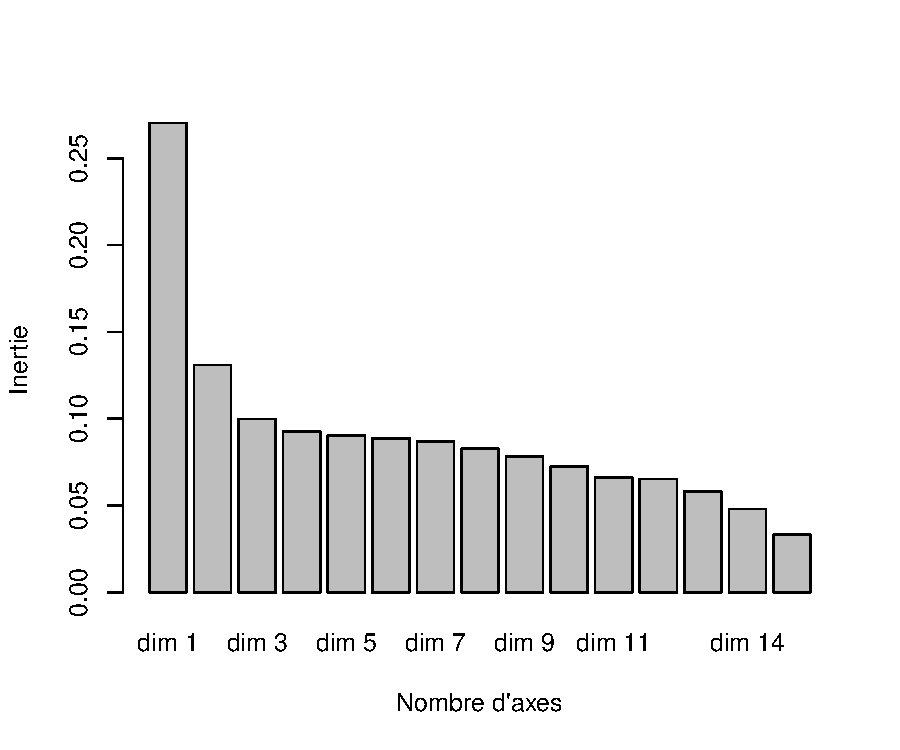
\includegraphics[width=0.5\linewidth]{M2_ANTUNEZ_SQD_files/figure-latex/inertie1-1}

\captiontmp[Inertie conservée selon le nombre d'axes de l'ACM]{Inertie conservée selon le nombre d'axes de l'ACM}\label{fig:inertie1}

\footnotesize
\normalsize\end{center}

\textbf{Classification Ascendante Hiérarchique}

La Classification Ascendante Hiérarchique est une méthode de classification très fréquemment effectuée à la suite d'une ACM pour rassembler les individus en groupes (appelés classes) qui se distinguent fortement selon des critères socialement interprétables. Nous avons appliqué cette méthode sur les deux premiers axes de l'ACM obtenue précédemment.

Le choix du nombre de classes n'est pas imposé par la méthode. Nous avons choisi une classification en 5 classes, car ce seuil correspond à un fort saut d'inertie du dendrogramme (figure \ref{fig:inertie2}). Il s'agit également d'un nombre de classes suffisamment important pour présenter des différences marquées dans l'interprétation des classes, classes qui sont par ailleurs de tailles suffisantes pour être interprétées (7,4 \% à 30,7 \% de l'échantillon).
\begin{center} 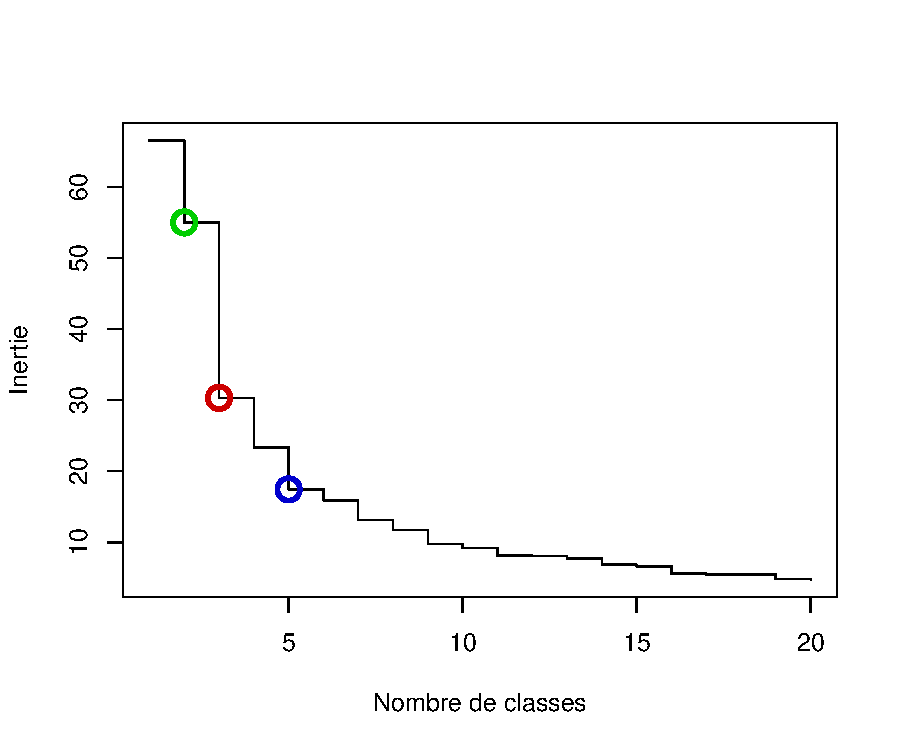
\includegraphics[width=0.5\linewidth]{M2_ANTUNEZ_SQD_files/figure-latex/inertie2-1}

\captiontmp[Inertie conservée selon le nombre de classes de la CAH]{Inertie conservée selon le nombre de classes de la CAH}\label{fig:inertie2}

\footnotesize
\normalsize\end{center}

\end{summary_box}
\begin{figure}[!ht]

{\centering 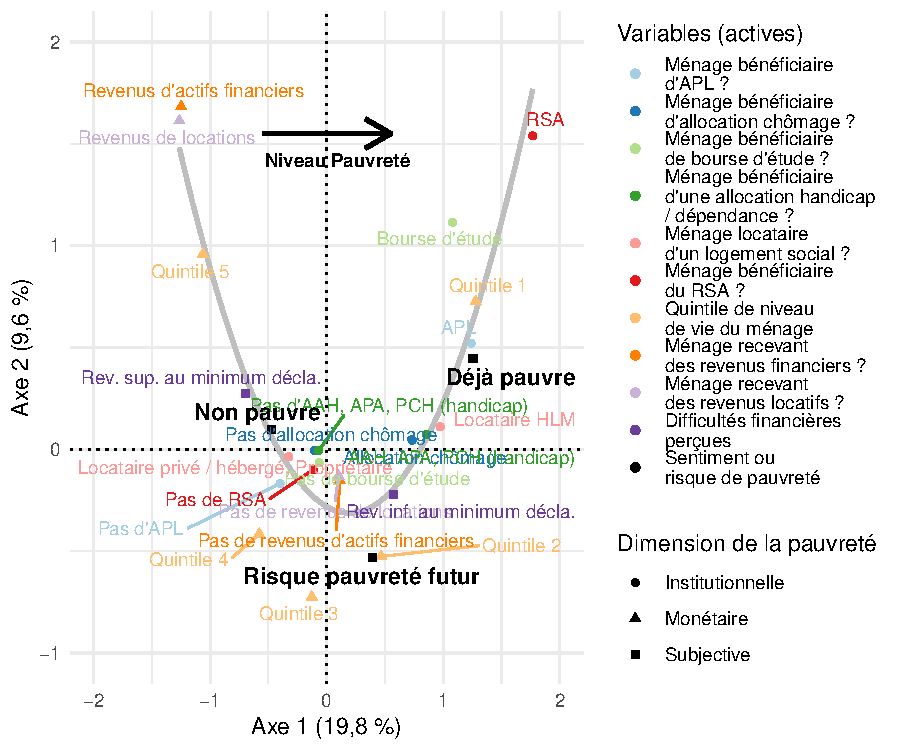
\includegraphics[width=1\linewidth]{M2_ANTUNEZ_SQD_files/figure-latex/acm1-1} 

}

\caption[Espace des variables actives de la pauvreté monétaire, institutionnelle et sujective (ACM)]{Espace des variables actives de la pauvreté monétaire, institutionnelle et sujective (ACM)}\label{fig:acm1}

\footnotesize


\emph{Source} : \emph{Baromètre d’opinion de la DREES, 2015-2019.}


\emph{Champ} : \emph{Personnes d’au moins 18 ans résidant en France métropolitaine.}


\emph{Note} : \emph{Pour cette étude, 1 798 individus sur les 15 137 individus étudiés au total ont été retirés du champ car ils ne se sont pas prononcés sur au moins une des questions étudiées (en variables actives ou supplémentaires).}
\normalsize\end{figure}

La figure \ref{fig:acm2} projette sur le nuage des variables les modalités de quatre variables supplémentaires particulièrement intéressantes à analyser : l'année, le niveau de diplôme, la situation vis-à-vis du marché du travail et la structure du ménage. Leur position situe les différents groupes sociaux dans l'espace de pauvreté.

Tout d'abord, les différentes années se situent au centre des deux axes, indiquant que, même si les années 2018 et 2019 se distinguent par une hausse du sentiment de pauvreté (comme vu dans la section \ref{sec:augmentesubj}), globalement aucune année ne se distingue par une situation de pauvreté plus importante sur l'ensemble des variables actives. Ainsi, l'espace social de la pauvreté est globalement structuré chaque année de la même manière depuis 2015\footnote{Nous avons également réalisé, en plus de cette ACM, deux ACM identiques à cette première mais une s'intéressant uniquement aux données avant 2018 (exclu) et l'autre après 2018 (inclus). Les deux nuages obtenus étaient très semblables à celui-ci, ce qui va dans le sens de l'analyse faite à partir de la figure \ref{fig:acm2}.}.
\begin{figure}[!ht]

{\centering 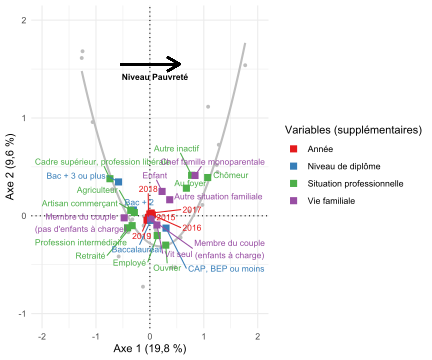
\includegraphics[width=1\linewidth]{M2_ANTUNEZ_SQD_files/figure-latex/acm2-1} 

}

\caption[Espace de quelques variables supplémentaires de la pauvreté monétaire, institutionnelle et sujective (ACM)]{Espace de quelques variables supplémentaires de la pauvreté monétaire, institutionnelle et sujective (ACM)}\label{fig:acm2}

\footnotesize


\emph{Source} : \emph{Baromètre d’opinion de la DREES, 2015-2019.}


\emph{Champ} : \emph{Personnes d’au moins 18 ans résidant en France métropolitaine.}


\emph{Note} : \emph{Pour cette étude, 1 798 individus sur les 15 137 individus étudiés au total ont été retirés du champ car ils ne se sont pas prononcés sur au moins une des questions étudiées (en variables actives ou supplémentaires).}
\normalsize\end{figure}

Par ailleurs, les personnes particulièrement exposées à la pauvreté (toutes dimensions confondues) semblent être les chefs de famille monoparentales, les chômeurs et autres inactifs non retraités et, dans une moindre mesure, les ouvriers et employés. Si un faible niveau de diplôme ne se confond pas avec la pauvreté telle qu'identifiée dans cet espace social, un très haut niveau de diplôme assure en revanche d'appartenir aux ménages les plus aisés.

\hypertarget{sec:esexplodescriCAH}{%
\subsection{Cinq classes ordonnées de pauvreté par Classification Ascendante Hiérarchique}\label{sec:esexplodescriCAH}}

Une Classification Ascendante Hiérarchique réalisée sur les deux premiers axes de la précédente ACM permet de regrouper les individus en 5 classes (voir encadré 1) représentées en figure \ref{fig:cah1}.
\begin{figure}[!ht]

{\centering 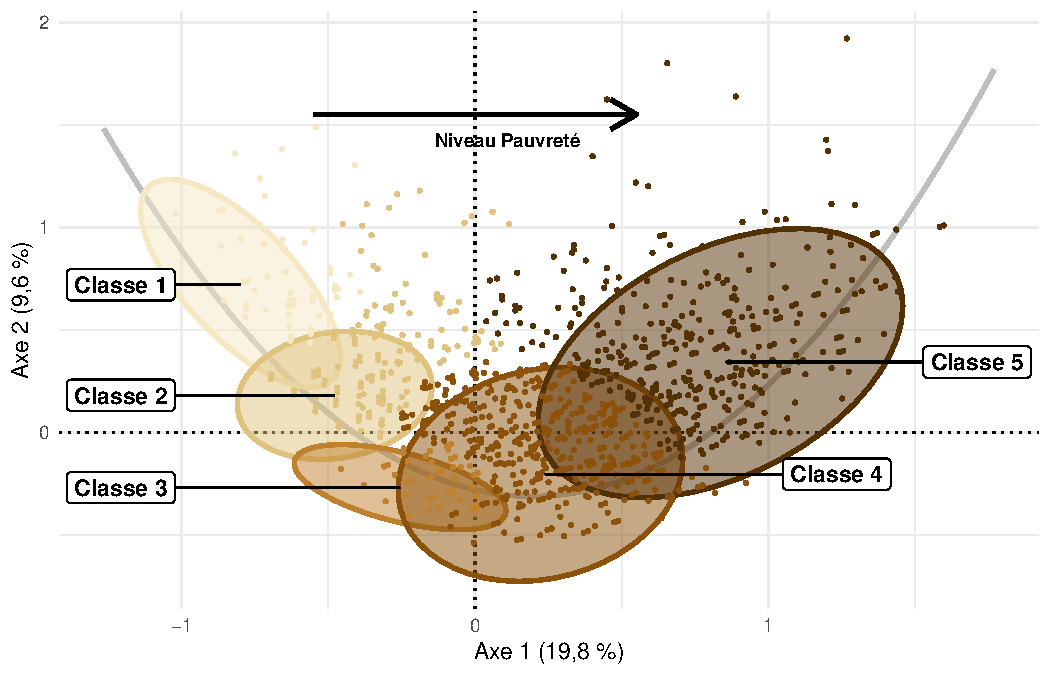
\includegraphics[width=1\linewidth]{M2_ANTUNEZ_SQD_files/figure-latex/cah1-1} 

}

\caption[Nuage des individus de l'ACM et CAH sur les deux premiers axes factoriels]{Nuage des individus de l'ACM et CAH sur les deux premiers axes factoriels}\label{fig:cah1}

\footnotesize


\emph{Source} : \emph{Baromètre d’opinion de la DREES, 2015-2019.}


\emph{Champ} : \emph{Personnes d’au moins 18 ans résidant en France métropolitaine.}


\emph{Note} : \emph{Le nuage des individus comporte beaucoup moins de points qu’il y a d’individus dans la base de données. C’est parce que de nombreux individus ont répondu exactement les mêmes réponses aux questions correspondant aux variables actives. Ils sont donc superposés sur cette figure.}
\normalsize\end{figure}
\begin{figure}[!ht]

{\centering 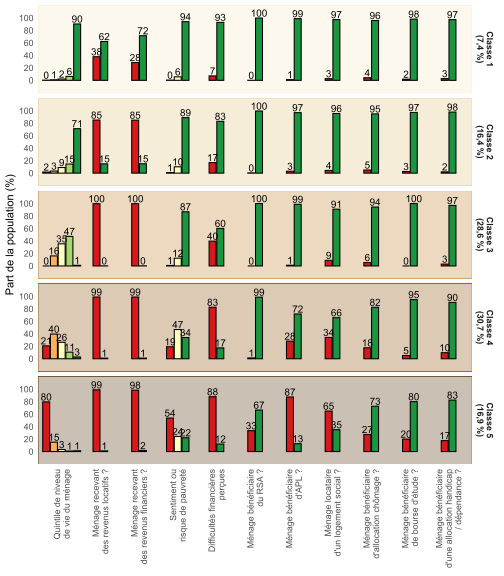
\includegraphics[width=1\linewidth]{M2_ANTUNEZ_SQD_files/figure-latex/cah2-1} 

}

\caption[Indicateurs des différentes dimensions de la pauvreté pour chacune des 5 classes de la CAH]{Indicateurs des différentes dimensions de la pauvreté pour chacune des 5 classes de la CAH}\label{fig:cah2}

\footnotesize


\emph{Source} : \emph{Baromètre d’opinion de la DREES, 2015-2019.}


\emph{Champ} : \emph{Personnes d’au moins 18 ans résidant en France métropolitaine.}


\emph{Note de lecture} : \emph{A structure familiale fixée, le fait d'indiquer percevoir soi-même le RSA multiplie par 7 les chances d'indiquer se sentir pauvre. Le percevoir au niveau de son ménage, multiplie les chances par 5.}
\normalsize\end{figure}

Plus précisément, la figure \ref{fig:cah2} permet de décrire l'importance de chacun des indicateurs de pauvreté dans chacune des cinq classes (tableau \ref{tab:tabclasses1})
\begin{longtable}[t]{>{}l>{\raggedright\arraybackslash}p{11cm}}
\caption{\label{tab:tabclasses1}Description des 5 classes ordonnées de pauvreté}\\
\toprule
Classe & Description\\
\midrule
\textbf{Classe 1} & Cette classe rassemble les individus les plus aisés de l’échantillon. \textbf{9 individus sur 10 appartiennent à un ménage du dernier quintile de niveau de vie}. Ils sont également majoritaires à recevoir des revenus issus de location ou d’actifs financiers. Aucun individu indique se sentir pauvre et seulement 7 \% indiquent disposer d’un revenu inférieur au minimum qu’il faut, selon eux, pour vivre.\\
\textbf{Classe 2} & Cette classe rassemble également des individus aisés. Cette fois-ci, seuls \textbf{7 individus sur 10 appartiennent au dernier quintile de niveau de vie} et moins d’un individu sur 5 dispose dans son ménage de revenus financiers ou locatifs.\\
\textbf{Classe 3} & Cette classe rassemble majoritairement des \textbf{individus appartenant aux troisième (35 \%) ou quatrième (47 \%) quintiles de niveau de vie} des ménages. S’ils sont aussi très peu nombreux à recevoir des aides sociales, ils sont 4 sur 10 à indiquer que leur revenu est inférieur au minimum qu’il faut, selon eux, pour vivre.\\
\textbf{Classe 4} & Cette classe est celle qui rassemble le plus d’individus appartenant au \textbf{deuxième quintile de niveau de vie des ménages} (4 sur 10). 19 \% d’entre eux indiquent se sentir pauvre, près de la moitié indiquant en revanche risquer le devenir dans les cinq prochaines années. Une minorité d’individus dispose d’APL (28 \%), d’un logement social (34 \%) ou d’une allocation chômage (18 \%) et seuls 1 \% sont bénéficiaires du RSA.\\
\textbf{Classe 5} & Cette classe est celle qui rassemble le plus d’individus appartenant au \textbf{premier quintile de niveau de vie} des ménages (8 sur 10). Ils sont plus de la moitié à se sentir pauvre et près d’un quart à indiquer risquer le devenir dans les cinq prochaines années. Une large majorité d’individus dispose d’aides sociales en particulier d’APL (87 \%), d’un logement social (65 \%) ou du RSA (33 \%).\\
\bottomrule
\end{longtable}
Sans surprise, ces 5 classes s'alignent et s'ordonnent selon la parabole de l'effet Guttman, les individus les plus à gauche (classe 1) correspondant aux individus les plus aisés et les plus à droite (classe 5) aux individus les plus modestes.

\hypertarget{sec:esexplostructu}{%
\section{Modèle structurel : les dimensions latentes de la pauvreté}\label{sec:esexplostructu}}

\hypertarget{sec:esexplostructuefa}{%
\subsection{Deux dimensions latentes par analyse en facteurs communs exploratoire}\label{sec:esexplostructuefa}}

L'effet Guttman observé en figure \ref{fig:acm1} suggère une corrélation globale entre l'ensemble des indicateurs de pauvreté. On pourrait alors en théorie classer les individus selon une échelle unidimensionnelle de la pauvreté (typiquement selon le premier axe de l'ACM). Toutefois, le chapitre \ref{nonreducnv} a montré que cette corrélation entre indicateurs et dimensions de la pauvreté n'est pas parfaite puisqu'à niveau de vie constant, la pauvreté institutionnelle et d'autres facteurs sociodémographiques influent sur le sentiment de pauvreté.

Remarquons par ailleurs que les corrélations de Spearman\footnote{La corrélation de Spearman permet de comparer deux variables sans que la relation soit nécessairement affine. Elle est égale au coefficient de corrélation de Pearson calculé sur les variables de rang. \(r_s = \mathrm{corr}(\mathrm{rg}_X, \mathrm{rg}_Y) = \frac{\mathrm{cov}(\mathrm{rg}_X, \mathrm{rg}_Y)}{\sigma_{\mathrm{rg}_X} \sigma_{\mathrm{rg}_Y}}\). La variable de rang \(\mathrm{rg}_{X_i}\) est définie telle que \(\mathrm{rg}_{X_i}=j \iff X_i = X_{(j)}\) (\(X_i\) est la \(j\)ème plus petite variable).} (figure \ref{fig:corrplot}) entre les différentes variables de pauvreté, ne sont, étonnamment, pas très élevées. Seule la corrélation entre niveau de vie (dimension monétaire) et difficultés financières perçues (dimension subjective) est significative au seuil de 5 \%. En abaissant le seuil de tolérance et en représentant l'ensemble des corrélations supérieures au seuil de corrélation (arbitraire) de 0,3 (figure \ref{fig:corrplot}), les deux indicateurs subjectifs ont une corrélation au-dessus de ce seuil, de même pour les corrélations entre variables institutionnelles de RSA, APL et de location d'un logement social prises deux à deux (sauf entre RSA et location d'un logement social). Conformément aux observations du chapitre précédent, le niveau de vie est central dans l'analyse de la pauvreté puisque corrélé avec les deux variables de pauvreté subjective et certaines variables de pauvreté institutionnelle (APL, location d'un logement social).
\begin{figure}[!ht]

{\centering 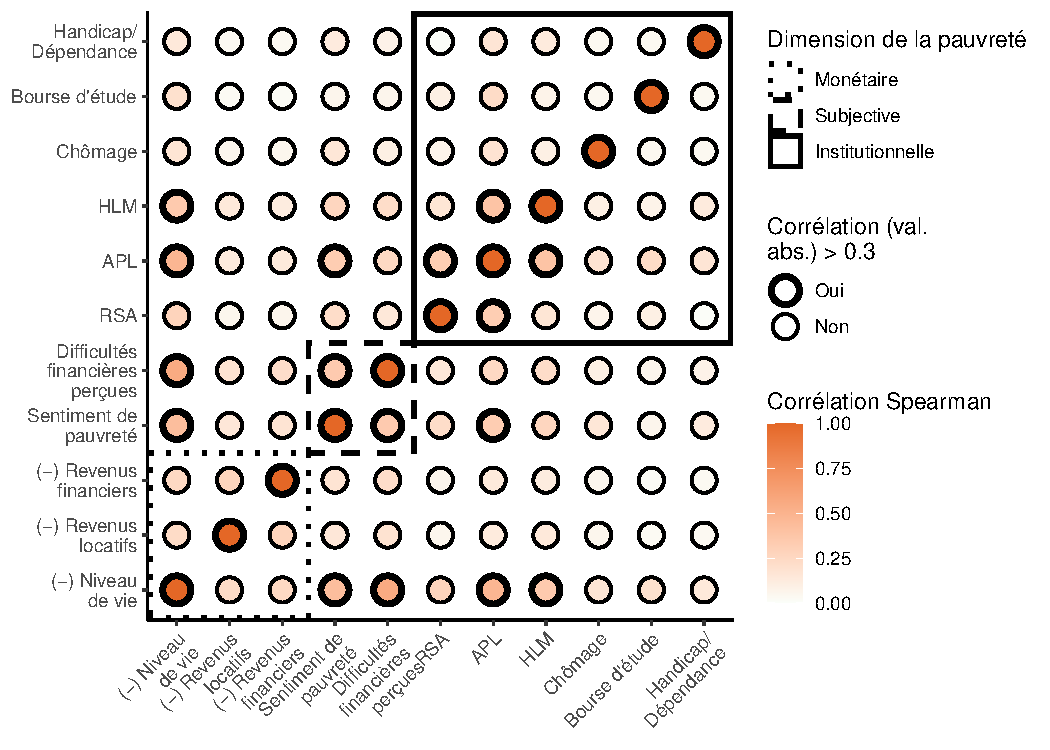
\includegraphics[width=1\linewidth]{M2_ANTUNEZ_SQD_files/figure-latex/corrplot-1} 

}

\caption[Corrélation de Spearman entreles différents indicateurs de pauvreté]{Corrélation de Spearman entreles différents indicateurs de pauvreté}\label{fig:corrplot}

\footnotesize


\emph{Source} : \emph{Baromètre d’opinion de la DREES, 2015-2019.}


\emph{Champ} : \emph{Personnes d’au moins 18 ans résidant en France métropolitaine.}
\normalsize\end{figure}

La figure \ref{fig:corrplot} illustre donc assez bien la complexité de l'espace social de la pauvreté, c'est-à-dire à la fois la corrélation qu'il existe entre certains indicateurs au sein d'une même dimension (mais pas tous !) mais aussi celle qui lie certains indicateurs appartenant à des dimensions différentes, en particulier le niveau de vie et les indicateurs de pauvreté subjective ainsi qu'avec le fait d'être bénéficiaire de certaines prestations sociales.
\begin{summary_box}[false]{Analyse en Facteurs communs et classes latentes}

\textbf{Analyse en Facteurs communs Exploratoire}

Alors que l'ACM avait pour principal objectif la réduction de la dimension des données, l'AFE cherche en outre à identifier des variables latentes -- typiquement les différentes dimensions de la pauvreté -- qui se cachent derrière les indicateurs mesurés dans la base de données. Par ailleurs, contrairement à l'ACM, elle conserve la structure des corrélations entre indicateurs (figure \ref{fig:corrplot}) et ne s'intéresse pas uniquement à la variance. La variance totale se décompose en effet en une somme de deux variances :
\begin{enumerate}
\def\labelenumi{\arabic{enumi}.}
\item
  la variance commune (\emph{communality}) qui correspond à la variance partagée par tous les indicateurs d'un même facteur (c'est-à-dire d'une même variable latente) ;
\item
  la variance unique (inexistante dans le cas d'une ACM) : celle spécifique à chaque indicateur (par exemple la variance spécifique du fait de toucher le RSA au-delà de la variance attribuable à la pauvreté institutionnelle) et celle due aux éventuelles erreurs de mesures.
\end{enumerate}
De nombreux détails sur l'AFE sont disponibles en annexe \ref{sec:annexeAFAFE}, avec, en outre, ses différences avec les méthodes d'analyse factorielle plus connues en France (type ACM) (voir annexe \ref{sec:annexeAFACMcompa}).

Nous avons réalisé l'AFE grâce à la fonction \texttt{psych::fa()} du logiciel R. La méthode factorielle qui a été utilisée est celle du maximum de vraisemblance (\texttt{fm=ml}) et la méthode de rotation a été choisie oblique (\texttt{rotate\ =\ "oblimin"}). Les corrélations sont de type polychloriques (\texttt{cor="poly"}) car adaptées aux variables polytomiques (à plusieurs modalités, \emph{polytomous} en anglais), comme celles dont nous disposons. Enfin, les scores factoriels sont calculés en réalisant une régression (\texttt{scores="regression"}).

Nous avons choisi de ne retenir que deux facteurs car, premièrement, le \emph{scree plot} (diagramme des valeurs des valeurs propres par facteurs) nous invitait à le faire (saut très élevé entre 1 et 2 facteurs et très faible entre 2 et 3 facteurs) et deuxièmement car les modèles avec davantage de facteurs apportaient peu en termes d'interprétation. Le modèle à trois facteurs isolait l'effet de recevoir des revenus financiers ou locatifs et celui à quatre facteurs isolait l'effet de percevoir le RSA.

\textbf{Classes latentes}

Nous avons ensuite estimé un modèle en 6 classes latentes sur indicateurs polytomiques grâce à la fonction \texttt{poLCA::poLCA()}. Le choix de 6 classes a été fait principalement selon un critère d'interprétabilité, puisque les indicateurs de qualité du modèle continuaient de s'améliorer même pour un nombre de classe élevé (tableau ci-dessous) dont les tailles étaient hétérogènes. Par exemple, le modèle à 8 classes, qui présentent un AIC et un BIC plus faible que le modèle à 6 classes, comportait une classe qui rassemblait uniquement 2 \% de l'échantillon.
\begin{tabular}{>{\raggedleft\arraybackslash}p{1.2cm}|>{\raggedleft\arraybackslash}p{2cm}|>{\raggedleft\arraybackslash}p{2cm}|>{\raggedleft\arraybackslash}p{1.1cm}|>{\raggedleft\arraybackslash}p{1.1cm}|>{\raggedleft\arraybackslash}p{1.5cm}|>{\raggedleft\arraybackslash}p{1.5cm}}
\hline
Nombre de classes & Valeur maximiale de la log-vraisemblance & Degrés de liberté des résidus & BIC & AIC & Ratio de vraisemblance & Chi2 de Pearson (données estimées versus observées)\\
\hline
2 & -72386 & 7648 & 145067 & 144834 & 7362 & 592820\\
\hline
3 & -70925 & 7632 & 142297 & 141944 & 4441 & 442716\\
\hline
4 & -70579 & 7616 & 141757 & 141284 & 3749 & 411225\\
\hline
5 & -70279 & 7600 & 141308 & 140715 & 3147 & 471387\\
\hline
6 & -70164 & 7584 & 141231 & 140519 & 2919 & 210385\\
\hline
7 & -70096 & 7568 & 141247 & 140415 & 2783 & 223124\\
\hline
8 & -69984 & 7552 & 141175 & 140222 & 2558 & 158915\\
\hline
\end{tabular}
\end{summary_box}
C'est pourquoi nous chercherons dans les parties qui suivent à aller plus loin dans la recherche d'axes de structuration / différenciation dans l'espace social de la pauvreté, dans l'idée d'analyser empiriquement en quoi elle est multidimensionnelle. Cette étude plus en profondeur de la structuration de l'espace social est permise par l'analyse en facteurs communs (AF) exploratoire (AFE) (encadré 2) qui permet de modéliser des variables latentes, c'est-à-dire, dans le cadre qui nous intéresse, les dimensions de la pauvreté.

La figure \ref{fig:afe} représente une AFE en deux facteurs (c'est-à-dire deux variables latentes) dont les résultats sont nets et facilement interprétables : le premier facteur rassemble les indicateurs de pauvretés monétaire et subjective et le second les indicateurs de pauvreté institutionnelle\footnote{L'indicatrice d'être bénéficiaire du RSA est relativement proche de la première bissectrice (saturation ou \emph{loading} de 0,52 pour le second axe et 0,23 pour le premier), de même pour la variable de location d'un logement social (0,46 contre 0,24), ce qui signifie qu'elles sont relativement proches également du premier facteur (dimensions monétaire ou subjective de la pauvreté).}. Les dimensions de la pauvreté sont ainsi non seulement théoriquement construites (cf.~partie \ref{chap1}) mais sont également validées empiriquement par AFE.
\begin{figure}[!ht]

{\centering 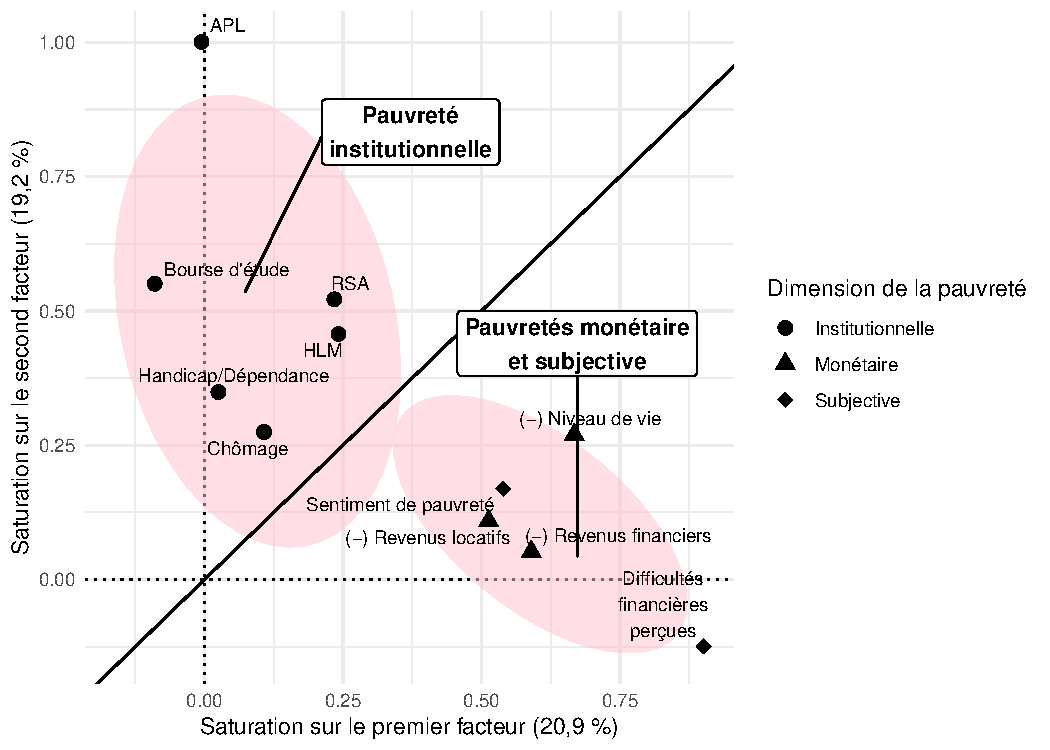
\includegraphics[width=1\linewidth]{M2_ANTUNEZ_SQD_files/figure-latex/afe-1} 

}

\caption[Espace des variables de pauvreté monétaire, institutionnelle et sujective (Analyse en Facteurs Communs Exploratoire)]{Espace des variables de pauvreté monétaire, institutionnelle et sujective (Analyse en Facteurs Communs Exploratoire)}\label{fig:afe}

\footnotesize


\emph{Source} : \emph{Baromètre d’opinion de la DREES, 2015-2019.}


\emph{Champ} : \emph{Personnes d’au moins 18 ans résidant en France métropolitaine.}


\emph{Note de lecture} : \emph{Pour la variable « HLM » (être locataire d’un logement social), la saturation sur le premier facteur est de 0,24 et celle sur le second facteur est de 0,46.}
\normalsize\end{figure}

Deux principales conclusions sont à tirer concernant l'espace social dessiné par AFE :
\begin{itemize}
\item
  La première est que ce résultat éclaire l'importance de la pauvreté institutionnelle soulignée par Paugam, puisque les indicateurs de pauvreté institutionnelle mesurés dans le Baromètre se rassemblent en une même dimension latente (le second facteur). Cette dimension est directement en lien avec les politiques publiques de lutte contre la pauvreté et la précarité.
\item
  La seconde est que pauvreté monétaire et subjective constituent empiriquement une même dimension latente. Ce n'est pas surprenant puisqu'on a vu plus haut que la corrélation entre difficultés financières perçues (subjective) et quintiles de niveau de vie du ménage (monétaire) est la plus élevée de toutes (figure \ref{fig:corrplot}). Ce fort lien valide la pertinence de l'utilisation statistique d'indicateurs de pauvreté subjective : ils sont non seulement globalement connectés à la réalité des difficultés financières vécues par les ménages mais apportent également de la nuance et des informations sur le halo de la pauvreté, comme ont pu le montrer les modèles économétriques du chapitre \ref{nonreducnv}.
\end{itemize}
\hypertarget{sec:esexplostructutypo}{%
\subsection{Six classes non ordonnées de pauvreté par modèle en classes latentes}\label{sec:esexplostructutypo}}

À partir des résultats de l'AFE en deux facteurs communs, nous avons réalisé un modèle en 6 classes latentes. Les résultats du modèle sont présentés en figure \ref{fig:latentclass1}. Afin de comparer la nouvelle typologie à celle obtenue précédemment par CAH et en analyser les différences, les classes ont été représentées sur le même nuage des individus : celui qui les projette sur les premiers axes de l'ancienne ACM.
\begin{figure}[!ht]

{\centering 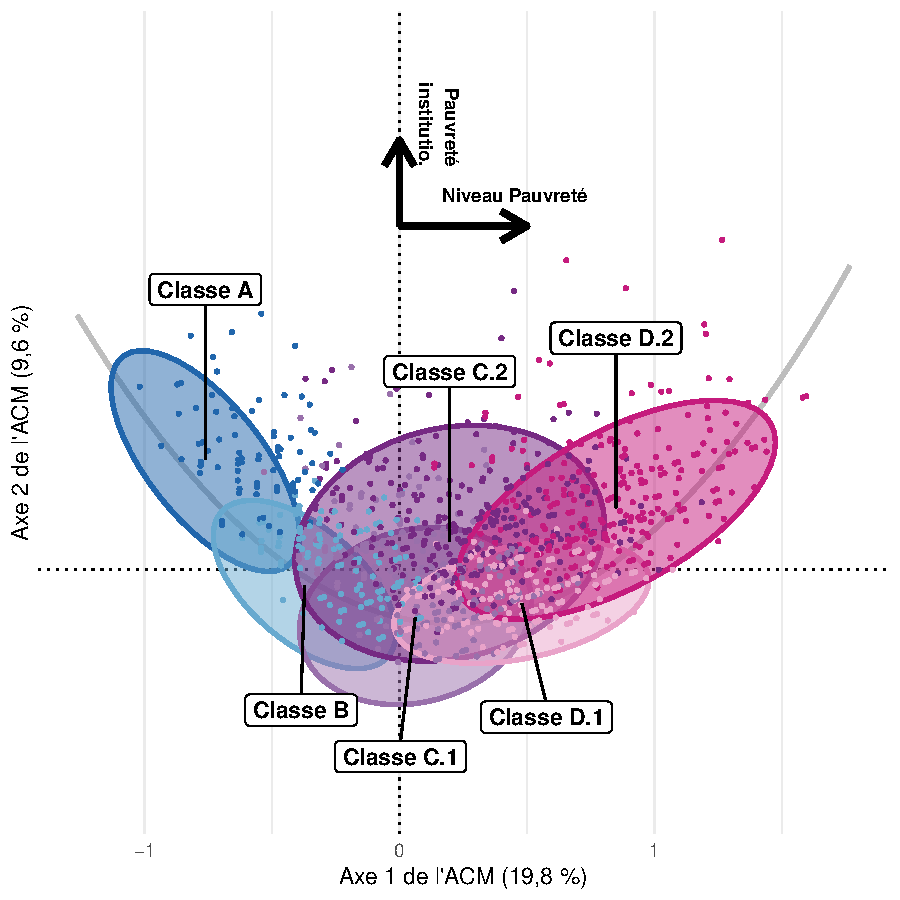
\includegraphics[width=1\linewidth]{M2_ANTUNEZ_SQD_files/figure-latex/latentclass1-1} 

}

\caption[Nuage des individus de l'ACM et classes latentes sur les deux premiers axes factoriels]{Nuage des individus de l'ACM et classes latentes sur les deux premiers axes factoriels}\label{fig:latentclass1}

\footnotesize


\emph{Source} : \emph{Baromètre d’opinion de la DREES, 2015-2019.}


\emph{Champ} : \emph{Personnes d’au moins 18 ans résidant en France métropolitaine.}
\normalsize\end{figure}

Les 6 classes obtenues s'ordonnent toujours globalement selon l'échelle de pauvreté qui correspond à la parabole de l'effet Guttman : les individus les plus à gauche (classes A et B) correspondent aux individus les plus aisés et à droite (classes C et D) aux individus les plus modestes. Toutefois, l'utilisation de l'analyse en facteurs communs permet d'ajouter de la nuance dans l'interprétation. En effet, deux paires de classes se situent au même niveau (pour C.1 et C.2) ou à un niveau proche (pour D.1 et D.2) sur l'échelle horizontale de pauvreté mais se distinguent en termes de structure de la pauvreté (positions verticales différentes).
\begin{figure}[!ht]

{\centering 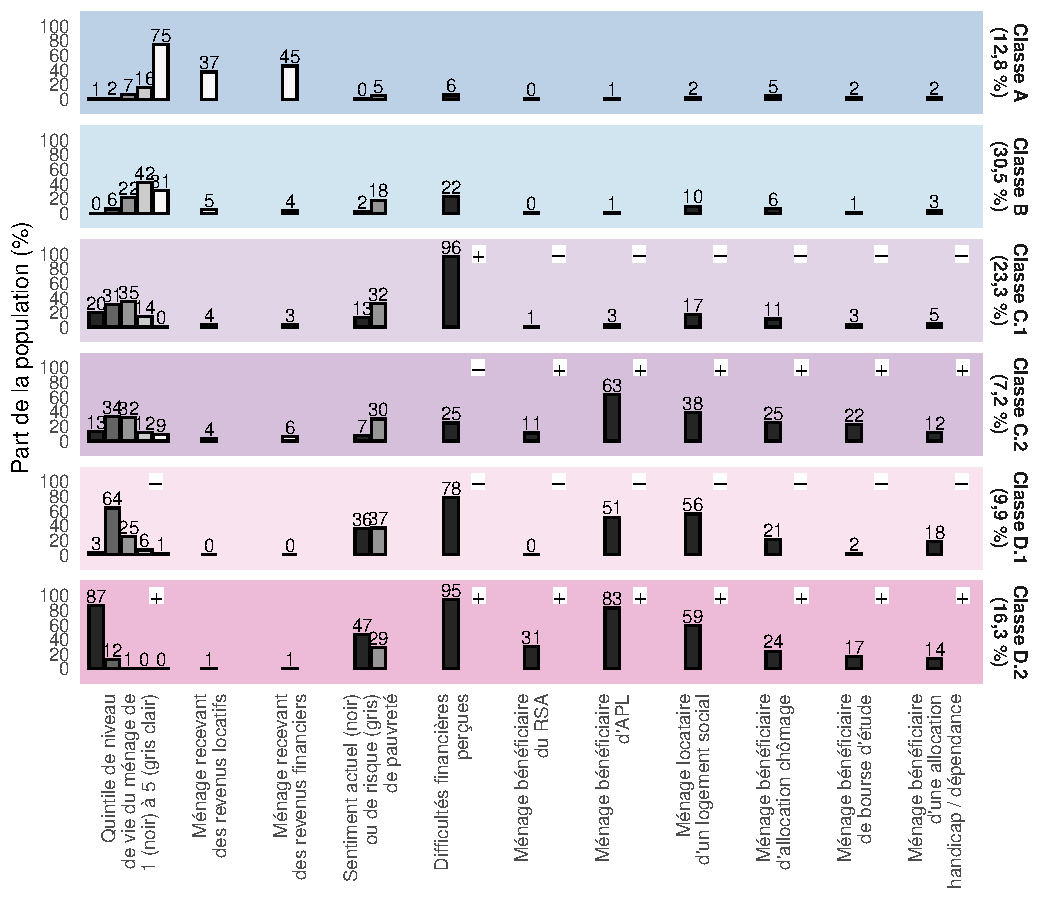
\includegraphics[width=1\linewidth]{M2_ANTUNEZ_SQD_files/figure-latex/latentclass2-1} 

}

\caption[Indicateurs des différentes dimensions de la pauvreté pour chacune des 6 classes latentes]{Indicateurs des différentes dimensions de la pauvreté pour chacune des 6 classes latentes}\label{fig:latentclass2}

\footnotesize


\emph{Source} : \emph{Baromètre d’opinion de la DREES, 2015-2019.}


\emph{Champ} : \emph{Personnes d’au moins 18 ans résidant en France métropolitaine.}


\emph{Note} : \emph{Dans la classe 3 qui rassemble 28,6 \% de l'échantillon, 35 \% des individus appartiennent à des ménages du troisième quintile de niveau de vie, aucun individu n’appartient à un ménage qui reçoit des revenus locatifs, 1 \% indiquent se sentir pauvre et 12 \% indiquent risquer le devenir dans les cinq prochaines années.}


\emph{Note de lecture} : \emph{Dans la classe B.1, 32 \% des individus appartiennent à des ménages du troisième quintile de niveau de vie, 4 \% des individus appartiennent à un ménage qui reçoit des revenus locatifs, 7 \% indiquent se sentir pauvre et 30 \% indiquent risquer le devenir dans les cinq prochaines années}
\normalsize\end{figure}

La figure \ref{fig:latentclass2} permet de décrire l'importance de chacune des dimensions de pauvreté dans chacune des six classes (tableau \ref{tab:tabclassesA}).
\begin{longtable}[t]{>{}l>{\raggedright\arraybackslash}p{11cm}}
\caption{\label{tab:tabclassesA}Description des 6 classes non ordonnées de pauvreté}\\
\toprule
Classe & Description\\
\midrule
\textbf{Classe A} & Comme les classes 1 voire 2 précédemment, cette classe rassemble les individus les plus aisés de l’échantillon. Les trois quarts des individus appartiennent à un ménage du dernier quintile de niveau de vie.\\
\textbf{Classe B} & Comme les classes 2 voire 3 précédemment, cette classe rassemble également des individus aisés. Cette fois-ci 7 individus sur 10 appartiennent aux deux derniers quintiles de niveau de vie.\\
\textbf{Classe C.1} & Cette classe rassemble majoritairement des individus appartenant aux \textbf{deuxième et troisième quintiles} de niveau de vie (7 individus sur 10) qui ne se sentent majoritairement pas pauvres (54 \%) mais sont toutefois respectivement 32 \% et 13 \% à penser le devenir ou l’être déjà. Ils ont \textbf{presque tous} la sensation d’avoir un \textbf{revenu inférieur au minimum} pour vivre et \textbf{ne reçoivent pas} de \textbf{prestations sociales}.\\
\textbf{Classe C.2} & Comme la classe C.1, cette classe rassemble majoritairement des individus appartenant au \textbf{deuxième et troisième quintiles} de niveau de vie (7 individus sur 10) mais sont toutefois respectivement 30 \% et 7 \% à penser le devenir ou l’être déjà. Ils sont \textbf{seulement un quart} à avoir la sensation d’avoir un \textbf{revenu inférieur au minimum} pour vivre et sont \textbf{assez nombreux à recevoir} des \textbf{prestations sociales}.\\
\textbf{Classe D.1} & Cette classe rassemble majoritairement des individus appartenant au \textbf{deuxième quintile} de niveau de vie (6 individus sur 10). 36 \% se sentent pauvres et 37 \% pensent risquer le devenir dans les cinq prochaines années et 78 \% se sentent en difficultés financières. Ils sont \textbf{assez nombreux} à recevoir des \textbf{prestations sociales}.\\
\addlinespace
\textbf{Classe D.2} & Cette classe rassemble majoritairement des individus appartenant au \textbf{premier quintile} de niveau de vie (9 individus sur 10). 47 \% se sentent pauvres et 29 \% pensent risquer le devenir dans les cinq prochaines années et 95 \% se sentent en difficultés financières. Ils sont \textbf{très nombreux} à percevoir des \textbf{prestations sociales}.\\
\bottomrule
\end{longtable}
Les classes C.2 et D.2 sont caractérisées par une présence plus importante de la pauvreté institutionnelle que les classes C.1 et D.1 (respectivement) alors que le niveau de pauvreté monétaire y est pourtant relativement comparable. Ce résultat traduit le rôle particulier joué par la pauvreté institutionnelle évoqué plus haut.

La comparaison des classes C.1 est C.2 est intéressante puisque, bien que la pauvreté institutionnelle soit plus forte dans la classe C.2 (en haut) que dans la classe C.1 (bas), cela ne se traduit pas par une plus forte perception de difficultés financières, bien au contraire. À l'inverse, les individus de la classe C.1 ne perçoivent pas de prestations sociales mais se sentent en difficulté financière. Contrairement à ce que l'on observe dans les classes populaires et aisées, dans les classes moyenne une opposition se crée entre pauvreté institutionnelle et subjective : ne pas être bénéficiaire de prestation sociale s'associe à un fort ressenti de difficulté financière, comme si ces prestations manquaient à une partie de la population des classes moyennes.

La comparaison entre les classes D.1 et D.2 se fait avec la même logique : la classe D.2 en situation de pauvreté institutionnelle plus importante. Toutefois, la classe D.2 se situe également plus à droite de la classe D.1 et son niveau de pauvreté global (en particulier monétaire) est alors également plus important, ce qui justifie une pauvreté institutionnelle plus forte que pour D.1.

\hypertarget{sec:esexplostructufam}{%
\subsection{La structure familiale, variable clef de la structuration de l'espace social de la pauvreté}\label{sec:esexplostructufam}}

La classification en 6 classes obtenue en figure \ref{fig:latentclass1} invite à s'interroger sur les différences sociales qui existent entre les deux classes moyennes C.2 -caractérisée par une forte présence de pauvreté institutionnelle mais par un ressenti de difficultés financières moindre) et C.1 (situation inverse). C'est pourquoi nous avons réalisé une nouvelle régression logistique pour laquelle la variable dépendante est l'appartenance à la classe C.2 plutôt que C.1. Les variables explicatives sont les différentes variables sociodémographiques déjà étudiées auparavant, en contrôlant également par le niveau de vie.

Le tableau \ref{tab:tablatent} présente les résultats de cette régression. Les classes moyennes concernées par la pauvreté institutionnelle (et par des difficultés financières subjectives moindres) sont les ménages jeunes, locataires, inactifs ou indiquant occuper un emploi précaire. Mais c'est en particulier la situation familiale de ces ménages qui joue le plus grand rôle. La pauvreté institutionnelle concerne particulièrement les ménages avec enfants : que ce soit les couples ou, encore davantage, les familles monoparentales.
\begin{longtable}[t]{>{\raggedright\arraybackslash}p{4cm}>{\raggedright\arraybackslash}p{6cm}>{\raggedright\arraybackslash}p{4cm}}
\caption{\label{tab:tablatent}Influence des caractéristiques sociales sur l'appartenance à la classe C.2 plutôt que C.1}\\
\toprule
Modèle logit & Variable dépendante : appartenir à la classe C.2 plutôt que C.1 & Odds ratio\\
\midrule
\endfirsthead
\caption[]{\label{tab:tablatent}Influence des caractéristiques sociales sur l'appartenance à la classe C.2 plutôt que C.1 \textit{(suite)}}\\
\toprule
Modèle logit & Variable dépendante : appartenir à la classe C.2 plutôt que C.1 & Odds ratio\\
\midrule
\endhead
\midrule
\multicolumn{3}{r@{}}{\textit{(suite en page suivante...)}}\
\endfoot
\bottomrule
\multicolumn{3}{l}{\rule{0pt}{1em}\textit{Note: }}\\
\multicolumn{3}{l}{\rule{0pt}{1em}N = 4305 et $R^2$ ajusté = $28,1 \, \%$.}\\
\multicolumn{3}{l}{\rule{0pt}{1em}* : significatif au seuil de $5 \, \%$ ; ** : $1 \, \%$ ; *** : $0,1 \, \%$.}\\
\endlastfoot
Niveau de vie & Quintile 1 & 0,37***\\
 & Quintile 2 & Réf.\\
 & Quintile 3 & 0,86\\
 & Quintile 4 & 0,91\\
 & Quintile 5 & 101864863,01\\
\addlinespace
Logement & Locataire ou hébergé & Réf.\\
 & Propriétaire & 0,17***\\
Situation professionnelle & Agriculteur & 2,38\\
 & Artisan commerçant & 1,08\\
 & Profession intermédiaire & Réf.\\
\addlinespace
 & Cadre supérieur, profession libérale & 0,59\\
 & Employé & 1,08\\
 & Ouvrier & 0,66*\\
 & Chômeur & 1,44\\
 & Retraité & 0,98\\
\addlinespace
 & Au foyer & 2,88***\\
 & Autre inactif & 3,41***\\
Précarité de l'emploi & N'est pas personne en emploi précaire & Réf.\\
(subjective) & est personne en emploi précaire & 2,62***\\
Niveau de diplôme le plus élevé & CAP, BEP ou moins & 0,93\\
\addlinespace
 & Baccalauréat & Réf.\\
 & Bac + 2 & 0,93\\
 & Bac + 3 ou plus & 1,05\\
Classe d'âge & 18 à 29 ans & 1,98***\\
 & 30 à 39 ans & Réf.\\
\addlinespace
 & 40 à 49 ans & 0,97\\
 & 50 à 59 ans & 0,86\\
 & 60 à 69 ans & 0,63\\
 & 70 ans et plus & 0,24**\\
Situation familiale & Vit seul & 0,91\\
\addlinespace
 & Membre du couple (pas d’enfants à charge) & Réf.\\
 & Membre du couple (enfants à charge) & 3,57***\\
 & Chef famille monoparentale & 4,42***\\
 & Enfant & 0,87\\
 & Autre situation familiale & 1,9*\\
\addlinespace
Sexe & Femme & Réf.\\
 & Homme & 1,06\\
Année & 2015 & Réf.\\
 & 2016 & 1\\
 & 2017 & 1,24\\
\addlinespace
 & 2018 & 0,82\\
 & 2019 & 0,75\\*
\end{longtable}\footnotesize
\emph{Source} : \emph{Baromètre d’opinion de la DREES, 2015-2019.}

\emph{Champ} : \emph{Personnes d’au moins 18 ans résidant en France métropolitaine appartenant aux classes C.1 et C.2.}
\normalsize

Ces ménages avec enfants (qu'ils soient composés d'un ou deux parents) sont en effet ceux qui bénéficient le plus d'APL parmi les ménages modestes appartenant aux deux premiers quintiles de niveau de vie (tableau \ref{tab:tabprestaviefam}). Les familles monoparentales sont également très nombreuses en proportion à percevoir le RSA : trois fois plus que les personnes seules et que les couples avec enfants.
Cette forte influence de la structure du ménage sur la pauvreté institutionnelle se comprend aisément puisque la composition et les revenus des ménages pris en compte dans les critères d'éligibilité sont différents selon les prestations : prise en compte ou non des concubins ou uniquement des conjoints (PACS / mariage), prise en compte des ressources des autres membres du ménage, etc.

Le tableau \ref{tab:tabpauvviefam} avait montré plus haut que la pauvreté subjective (sentiment de pauvreté tout comme difficultés financières perçues) concerne également particulièrement les familles monoparentales. Toutefois, l'écart avec les autres types de ménages est moins fort que concernant la pauvreté institutionnelle. Notamment, les personnes vivant seules sont également très touchées par la pauvreté subjective, alors que bien moins souvent bénéficiaires d'APL ou de RSA, ce qui justifie l'effet positif et significatif de leur appartenance à la classe C.1 plutôt que C.2.
\begin{table}

\caption{\label{tab:tabprestaviefam}Être bénéficiaire de RSA et d'APL selon la situation familiale pour les personnes appartenant aux deux premiers quintiles de niveau de vie}
\centering
\begin{tabular}[t]{>{\raggedright\arraybackslash}p{6cm}|>{\raggedleft\arraybackslash}p{4cm}|>{\raggedleft\arraybackslash}p{4cm}}
\hline
Situation familiale & Part des bénéficiaires d'APL sans son ménage (\%) & Part des bénéficiaires du RSA dans son ménage (\%)\\
\hline
Chef famille monoparentale & 71 & 30\\
\hline
Autre & 53 & 14\\
\hline
Membre du couple (enfants à charge) & 51 & 11\\
\hline
Vit seul & 47 & 11\\
\hline
Enfant & 43 & 15\\
\hline
Membre du couple (pas d’enfants à charge) & 25 & 6\\
\hline
\textbf{Ensemble} & \textbf{48} & \textbf{13}\\
\hline
\end{tabular}
\footnotesize


\emph{Source} : \emph{Baromètre d’opinion de la DREES, 2015-2019.}


\emph{Champ} : \emph{Personnes dont le ménage appartient aux deux premiers quintiles de niveau de vie, d’au moins 18 ans résidant en France métropolitaine.}
\normalsize\end{table}

\hypertarget{esconfi}{%
\chapter{La pauvreté comme Espace social (analyse confirmatoire)}\label{esconfi}}

Grâce à différentes méthodes, les analyses exploratoires menées dans les chapitres \ref{nonreducnv} et \ref{esexplo} ont permis de tirer les grandes conclusions suivantes sur la structuration de l'espace social de la pauvreté :
\begin{enumerate}
\def\labelenumi{\arabic{enumi}.}
\item
  Les groupes sociaux particulièrement touchés par la pauvreté sont les familles monoparentales, les chômeurs et inactifs non retraités ;
\item
  Bien que la pauvreté soit multidimensionnelle, les différents indicateurs de pauvreté sont fortement corrélés ;
\item
  La pauvreté institutionnelle se distingue toutefois des dimensions monétaire et subjective. Ces deux dernières dimensions sont rendues proches par la corrélation forte entre niveau de vie (dimension monétaire) et difficultés financières perçues (dimension subjective) ;
\item
  La structure familiale (familles monoparentales et couples avec enfants) influe particulièrement sur la pauvreté institutionnelle car fait partie des principaux critères entrant en compte dans l'éligibilité aux prestations sociales.
\item
  Être à la tête d'une famille monoparentale, vivre seul, ne pas être propriétaire de son logement, être en dehors du marché du travail ou dans une moindre mesure être ouvrier ou employé, influent sur la pauvreté subjective.
\end{enumerate}
Pour clore les recherches effectuées pour ce mémoire, nous proposons ce dernier chapitre \ref{esconfi} qui apporte peu de nouveaux résultats mais présente l'avantage de mobiliser une méthodologie synthétique modélisant la structure globale du phénomène de pauvreté mais également l'influence relative de chacune des trois dimensions sur le phénomène global de pauvreté, ainsi que les groupes sociaux concernés. Il s'agit de l'Analyse en Facteurs communs Confirmatoire (AFC ; cf.~encadré 3).
\begin{summary_box}[true]{Analyse en Facteurs communs Confirmatoire}
Comme l'AFE, l'AFC modélise grâce à des facteurs latents les relations entre des variables observées. Son aspect confirmatoire vise en outre à valider des hypothèses structurales fournies par la littérature, dans notre cas la structuration de la pauvreté en trois dimensions : monétaire, institutionnelle et subjective. Plus de détails concernant l'AFC sont disponibles en annexe \ref{sec:annexeAFAFC}.

Nous avons réalisé les modèles d'AFC grâce à la fonction \texttt{lavaan::cfa()} du logiciel R. La méthode d'estimation utilisée est une nouvelle fois celle du maximum de vraisemblance. Le modèle 1 est orthogonal, c'est-à-dire qu'on considère que les différentes dimensions de la pauvreté ne sont pas corrélées entre elles. Sans surprise, ce modèle est non valide (cf.~indices d'ajustement du tableau qui suit) alors que les suivants (non-orthogonaux) le sont et sont de qualités globalement équivalentes.

\medskip
\begin{tabular}{l|r|r|l|l|l}
\hline
Modèle & Chi2 & Degrés de liberté & CFI & RMSEA & SRMR\\
\hline
Modèle 1 & 40598 & 44 & 0,243 & 0,263 & 0,286\\
\hline
Modèle 2 & 792 & 41 & 0,986 & 0,037 & 0,073\\
\hline
Modèle 3 & 590 & 33 & 0,985 & 0,036 & 0,077\\
\hline
Modèle 4 & 595 & 34 & 0,985 & 0,035 & 0,076\\
\hline
\end{tabular}
\medskip

\emph{Note : Pour que le modèle soit valide, on compare en général la valeur des indicateurs d'ajustement à certains seuils de référence. Le CFI doit être supérieur à 0,95. Le RMSEA doit être dans l'intervalle {[}0,05 ; 0,10{]}. Le SRMR doit être inférieur à 0,08. La p-valeur associée à l'indice du chi-2 doit être supérieure à 1 (attention, c'est contre-intuitif par rapport aux tests habituels), ce qui n'est jamais le cas ici (cas classique en cas de grosse base de données comme la nôtre).}

Ces modèles permettent également l'ajout de covariables externes (observées dans les données) dans le modèle. Ces modèles qualifiés de MIMIC (\emph{multiple indicators multiple causes model}). Ces ajouts permettent d'analyser l'influence du fait d'appartenir à certains groupes sociaux sur les différentes dimensions de la pauvreté.

\end{summary_box}
\hypertarget{sec:esconfiinter}{%
\section{Action des différentes formes de pauvreté dans les différents groupes sociaux}\label{sec:esconfiinter}}

Le premier modèle (figure \ref{fig:grviz1}) sert de point de départ puisqu'il considère les différentes dimensions de la pauvreté comme étant indépendantes. Cette hypothèse est fortement contestable comme ont pu le montrer les résultats des chapitres précédents. C'est pourquoi les statistiques d'ajustement (encadré 3) l'invalident totalement. Par ailleurs, la mauvaise qualité de l'estimation s'illustre également par la présence d'un « cas Heywood » (variance négative de l'indicateur d'APL dont la saturation devient alors supérieure à 1 ; annexe \ref{sec:annexeAFAFC}).
\begin{figure}[!ht]

{\centering 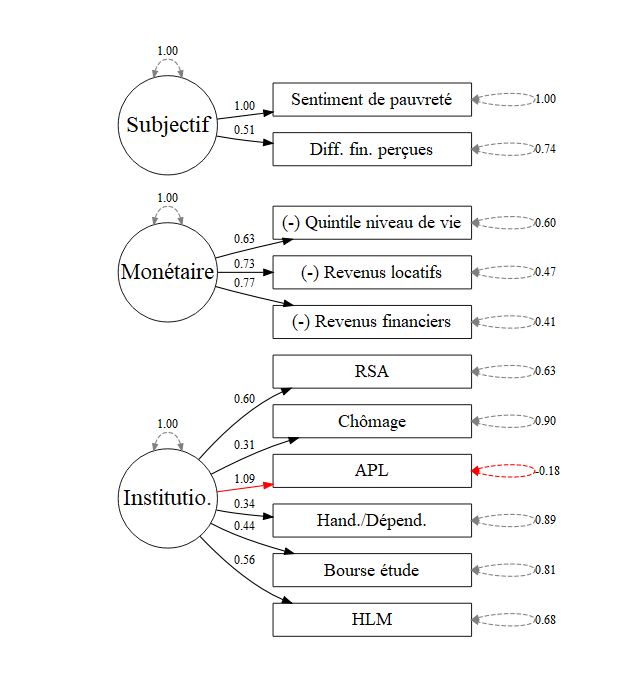
\includegraphics[width=0.8\linewidth]{M2_ANTUNEZ_SQD_files/figure-latex/grviz1-1} 

}

\caption[Modèle 1 ]{Modèle 1 : Modèle orthogonal}\label{fig:grviz1}

\footnotesize


\emph{Source} : \emph{Baromètre d’opinion de la DREES, 2015-2019.}


\emph{Champ} : \emph{Personnes d’au moins 18 ans résidant en France métropolitaine.}


\emph{Note} : \emph{Les variables encerclées correspondent aux variables latentes et les rectangulaires aux indicateurs observés dans la base de données. Les flèches en trait plein qui les relient correspondent aux saturations et les doubles flèches en pointillés aux variances. Les variances des facteurs fixées à 1 correspondent à des contraintes nécessaires pour que le modèle soit identifiable.}
\normalsize\end{figure}

Dans le deuxième modèle (figure \ref{fig:grviz2}), les corrélations entre facteurs sont autorisées et sont, d'ailleurs, très élevées. Les indices d'ajustement sont au vert et le cas Heywood de l'APL disparaît : sa saturation reste élevée (0,88) mais est bien inférieure à 1. Cette forte saturation, ainsi que celle de la location HLM qui suit de près celle du RSA (0,56 contre 0,60) indique à quel point la dimension du logement est très importante pour définir la pauvreté institutionnelle, c'est-à-dire la dépendance financière vis-à-vis de l'Etat, même s'il ne s'agit pas de minima sociaux à proprement parler.

En outre, deux saturations sont également particulièrement modifiées par rapport au modèle 1 : celles du quintile de niveau de vie et des difficultés financières perçues, qui augmentent fortement. Rappelons que ces deux variables, bien qu'appartenant à deux dimensions distinctes de la pauvreté (monétaire et subjective), font directement référence au revenu disponible, indicateur phare pour définir la pauvreté, et sont particulièrement corrélées (figure \ref{fig:corrplot}).
\begin{figure}[!ht]

{\centering 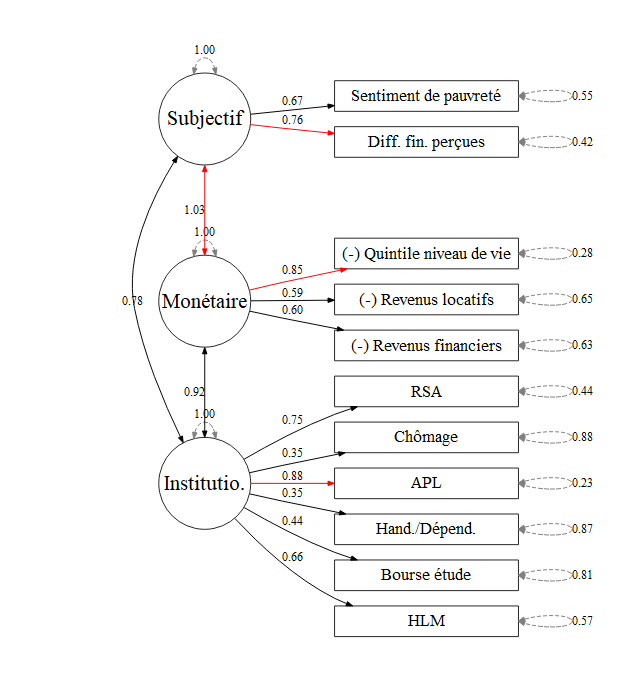
\includegraphics[width=0.8\linewidth]{M2_ANTUNEZ_SQD_files/figure-latex/grviz2-1} 

}

\caption[Modèle 2 ]{Modèle 2 : Modèle non-orthogonal}\label{fig:grviz2}

\footnotesize


\emph{Source} : \emph{Baromètre d’opinion de la DREES, 2015-2019.}


\emph{Champ} : \emph{Personnes d’au moins 18 ans résidant en France métropolitaine.}


\emph{Note} : \emph{Les variables encerclées correspondent aux variables latentes et les rectangulaires aux indicateurs observés dans la base de données. Les flèches en trait plein qui les relient correspondent aux saturations et les doubles flèches en pointillés aux variances. Les variances des facteurs fixées à 1 correspondent à des contraintes nécessaires pour que le modèle soit identifiable.}
\normalsize\end{figure}

Ainsi, quand on considère la pauvreté comme un ensemble de dimensions corrélées, le niveau de vie prend toute son importance. Cette forte corrélation entre les indicateurs de niveau de vie objectif et de difficultés financières perçues va même jusqu'à poser un problème de modélisation. La force de leur corrélation comparativement aux autres variables appartenant à un même facteur invalide l'hypothèse structurale que nous faisons de les classer dans deux dimensions différentes de la pauvreté. On le voit par la corrélation des dimensions subjective et monétaire qui est supérieure à 1 (figure \ref{fig:grviz2}) et fausse le modèle.

C'est pourquoi nous décidons d'enlever l'indicateur de difficultés financières perçues des modèles confirmatoires qui suivent, en particulier le modèle 3 (figure \ref{fig:grviz3}). La dimension subjective de la pauvreté est alors de fait supprimée puisqu'elle ne comporte plus qu'un indicateur observé : le sentiment de pauvreté.
\begin{figure}[!ht]

{\centering 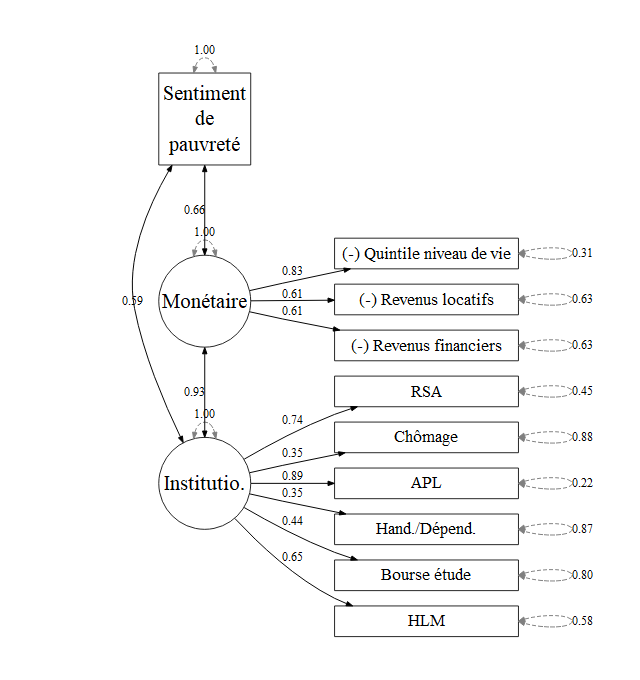
\includegraphics[width=0.8\linewidth]{M2_ANTUNEZ_SQD_files/figure-latex/grviz3-1} 

}

\caption[Modèle 3 ]{Modèle 3 : Modèle non-orthogonal sans les difficultés financières perçues}\label{fig:grviz3}

\footnotesize


\emph{Source} : \emph{Baromètre d’opinion de la DREES, 2015-2019.}


\emph{Champ} : \emph{Personnes d’au moins 18 ans résidant en France métropolitaine.}


\emph{Note} : \emph{Les variables encerclées correspondent aux variables latentes et les rectangulaires aux indicateurs observés dans la base de données. Les flèches en trait plein qui les relient correspondent aux saturations et les doubles flèches en pointillés aux variances. Les variances des facteurs fixées à 1 correspondent à des contraintes nécessaires pour que le modèle soit identifiable.}
\normalsize\end{figure}

Le modèle 3, dont les indices d'ajustement sont très bons et qui ne comporte plus de problème d'estimation, nous permet de complexifier encore davantage la modélisation en y ajoutant des variables de contrôle pour chacune des dimensions de la pauvreté, dont les coefficients sont présentés en tableau \ref{tab:tabinter} et dont certains sont représentés graphiquement en figure \ref{fig:ggradar} afin de faciliter leur interprétation.
\begin{longtable}[t]{>{\raggedright\arraybackslash}p{3cm}>{\raggedright\arraybackslash}p{2cm}>{\raggedright\arraybackslash}p{2.5cm}>{\raggedright\arraybackslash}p{2cm}l}
\caption{\label{tab:tabinter}Effets des covariables sur les différentes dimensions de la pauvreté}\\
\toprule
 & Pauvreté... & Monétaire & Institutionnelle & Sentiment de pauvreté\\
\midrule
\endfirsthead
\caption[]{\label{tab:tabinter}Effets des covariables sur les différentes dimensions de la pauvreté \textit{(suite)}}\\
\toprule
 & Pauvreté... & Monétaire & Institutionnelle & Sentiment de pauvreté\\
\midrule
\endhead
\midrule
\multicolumn{5}{r@{}}{\textit{(suite en page suivante...)}}\
\endfoot
\bottomrule
\multicolumn{5}{l}{\rule{0pt}{1em}\textit{Note: }}\\
\multicolumn{5}{l}{\rule{0pt}{1em}* : significatif au seuil de 5 \% ; ** : 1 \% ; *** : 0,1 \%.}\\
\endlastfoot
Situation professionnelle & Agriculteur & 0.39* & -0.49 & 0.24\\
 & Artisan commerçant & 0.06 & 0.03 & 0.07\\
 & Cadre supérieur, profession libérale & -0.36*** & -0.3*** & -0.16**\\
 & Profession intermédiaire & Réf. & Réf. & Réf.\\
 & Employé & 0.43*** & 0.53*** & 0.34***\\
\addlinespace
 & Ouvrier & 0.5*** & 0.53*** & 0.43***\\
 & Chômeur & 1.51*** & 1.57*** & 0.83***\\
 & Retraité & 0.58*** & 0.34*** & 0.13*\\
 & Au foyer & 1.23*** & 1.38*** & 0.53***\\
 & Autre inactif & 1.57*** & 1.6*** & 0.79***\\
\addlinespace
Niveau de diplôme le plus élevé & CAP, BEP ou moins & 0.57*** & 0.45*** & 0.29***\\
 & Baccalauréat & Réf. & Réf. & Réf.\\
 & Bac + 2 & -0.32*** & -0.21*** & -0.21***\\
 & Bac + 3 ou plus & -0.69*** & -0.36*** & -0.4***\\
Classe d'âge & 18 à 29 ans & 0.18*** & 0.18*** & -0.18***\\
\addlinespace
 & 30 à 39 ans & Réf. & Réf. & Réf.\\
 & 40 à 49 ans & -0.18*** & -0.12* & -0.07\\
 & 50 à 59 ans & -0.48*** & -0.3*** & -0.13***\\
 & 60 à 69 ans & -0.62*** & -0.65*** & -0.18**\\
 & 70 ans et plus & -0.74*** & -1.06*** & -0.4***\\
\addlinespace
Situation familiale & Vit seul & 0.71*** & 0.86*** & 0.54***\\
 & Membre du couple (pas d’enfants à charge) & Réf. & Réf. & Réf.\\
 & Membre du couple (enfants à charge) & 0.75*** & 0.7*** & 0.1**\\
 & Chef famille monoparentale & 1.57*** & 1.77*** & 0.71***\\
 & Enfant & 0.03 & 0.12 & 0.01\\
\addlinespace
 & Autre situation familiale & 0.8*** & 0.69*** & 0.41***\\
Sexe & Femme & Réf. & Réf. & Réf.\\
 & Homme & -0.13*** & -0.04 & -0.03\\*
\end{longtable}\footnotesize
\emph{Source} : \emph{Baromètre d’opinion de la DREES, 2015-2019.}

\emph{Champ} : \emph{Personnes d’au moins 18 ans résidant en France métropolitaine.}
\normalsize
\begin{figure}[!ht]

{\centering 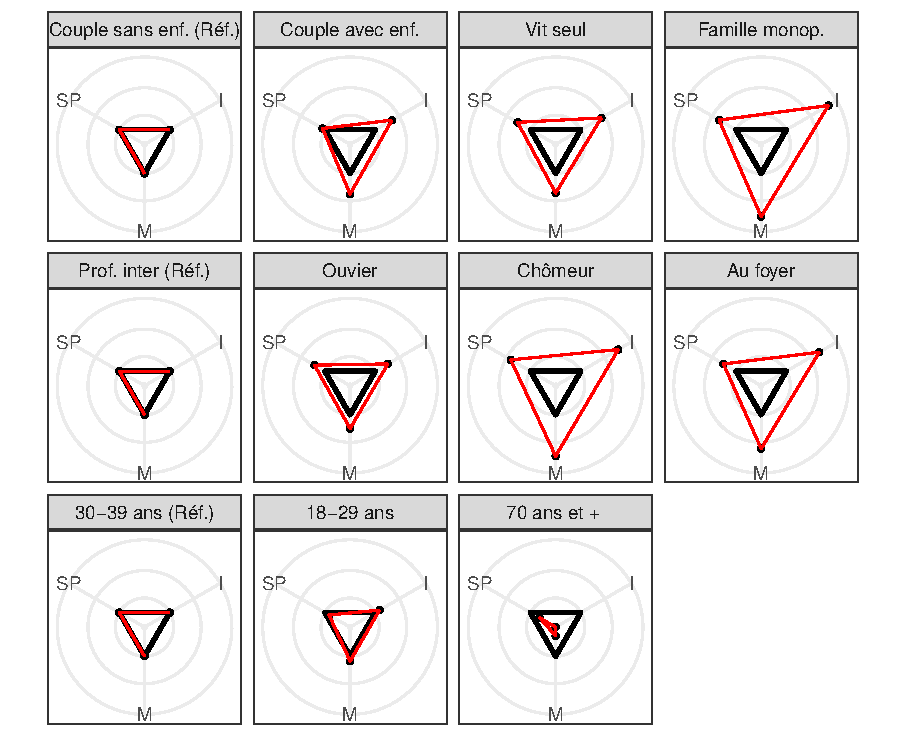
\includegraphics[width=1\linewidth]{M2_ANTUNEZ_SQD_files/figure-latex/ggradar-1} 

}

\caption[Représentation graphique de quelques coefficients du modèle 3 avec covariables]{Représentation graphique de quelques coefficients du modèle 3 avec covariables}\label{fig:ggradar}

\footnotesize


\emph{Champ} : \emph{Personnes d’au moins 18 ans résidant en France métropolitaine.}
\normalsize\end{figure}

Globalement, l'appartenance à un certain groupe social (selon l'âge, la situation d'emploi, familiale\ldots) a un effet plus marqué sur les dimensions objectives (monétaire et institutionnelle) que sur le sentiment de pauvreté. Bien que le fait d'être éloigné du marché du travail (chômeurs, personnes au foyer et autres inactifs) ait un effet non négligeable sur le sentiment de pauvreté, l'effet sur la pauvreté objective est bien plus fort. En revanche, être ouvrier en emploi augmente la pauvreté subjective à un niveau quasi-similaire que pour les deux dimensions objectives de la pauvreté.

En termes d'âge, appartenir à la tranche des 18-29 ans a un effet proche des 30-39 ans (référence) sur les 3 types de pauvreté. Toutefois, alors que l'effet sur les pauvretés objectives est légèrement positif, celui sur la pauvreté subjective est légèrement négatif. Le sentiment de pauvreté est ainsi particulièrement peu prononcé chez les plus jeunes. À l'inverse, être âgé de plus de 70 ans joue négativement sur le fait d'être pauvre, mais bien plus concernant les dimensions objectives que pour la dimension subjective.

Enfin, les effets sont, une nouvelle fois, très différenciés selon la situation familiale des répondants. Cela n'est pas surprenant puisque le niveau des prestations sociales -- et donc le niveau des revenus qui en découle -- est particulièrement conditionné par la structure familiale. Chez les chefs de famille monoparentale, les trois dimensions de la pauvreté sont élevées, mais particulièrement les deux dimensions objectives. Le niveau de la dimension subjective est comparable à celui des personnes qui vivent seules, qui se sentent particulièrement pauvres relativement à leur pauvreté objective bien moindre. Le niveau de pauvreté objective des personnes vivant seules est lui comparable à celui des couples avec enfant, qui, eux, se sentent bien moins pauvres.

\hypertarget{sec:esconfiglobal}{%
\section{Vers un indice synthétique de pauvreté}\label{sec:esconfiglobal}}

Pour finir, le modèle 4 (figure \ref{fig:grviz4}) ajoute un niveau hiérarchique supplémentaire et permet de définir le phénomène social de pauvreté par les trois dimensions étudiées dans ce mémoire : premièrement la dimension monétaire, la plus importante (saturation la plus élevée, valant 1), deuxièmement la dimension institutionnelle, défendue par Paugam (0,93) et, enfin, le sentiment de pauvreté (0,65) dont Papuchon et Duvoux ont également montré tout l'intérêt.

Nous avons fixé comme contraintes supplémentaires la saturation du quintile de niveau de vie (0,83) et celle du RSA (0,74) pour rendre le modèle comparable au modèle 3. Nous avons également dû corriger la variance de la pauvreté monétaire qui était négative (nouveau cas Heywood) en l'imposant légèrement positive afin que la saturation associée à la dimension monétaire reste inférieure à 1, pour assurer la validité du modèle.
\begin{figure}[!ht]

{\centering 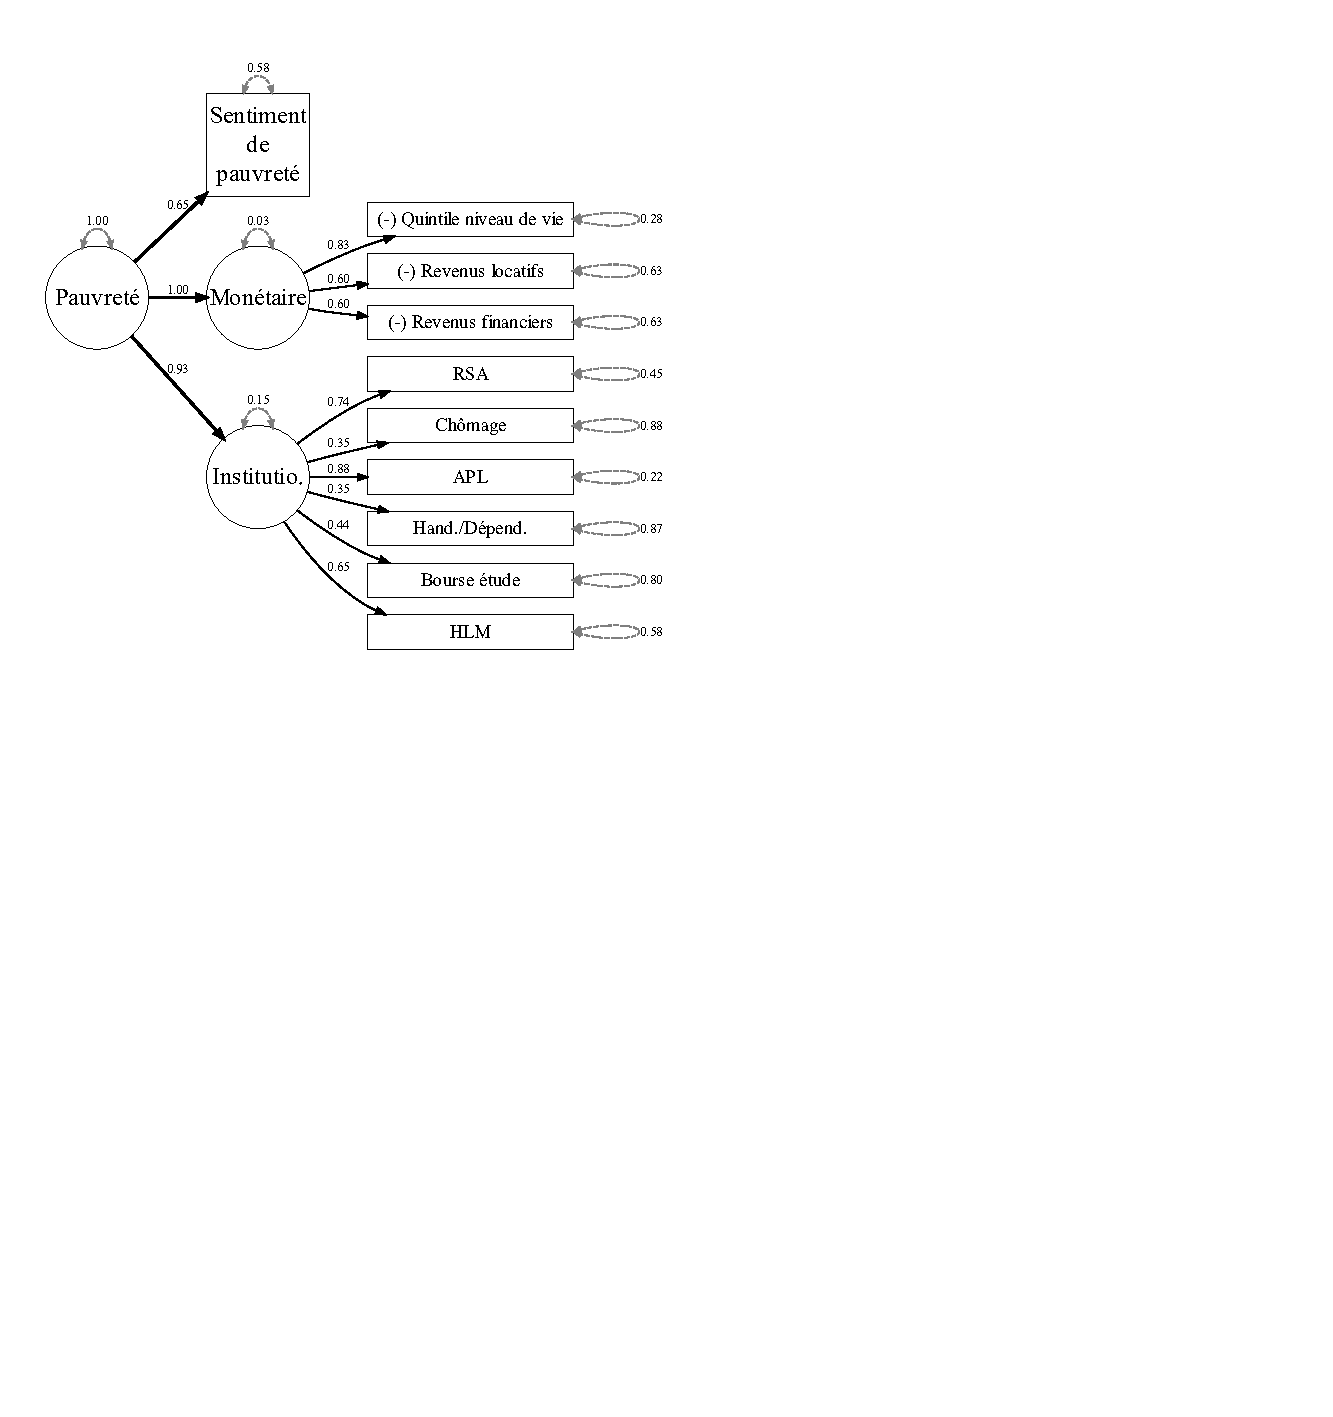
\includegraphics[width=0.8\linewidth]{M2_ANTUNEZ_SQD_files/figure-latex/grviz4-1} 

}

\caption[Modèle 4 ]{Modèle 4 : Modèle non-orthogonal sans les difficultés financières perçues}\label{fig:grviz4}

\footnotesize


\emph{Source} : \emph{Baromètre d’opinion de la DREES, 2015-2019.}


\emph{Champ} : \emph{Personnes d’au moins 18 ans résidant en France métropolitaine.}


\emph{Note} : \emph{Les variables encerclées correspondent aux variables latentes et les rectangulaires aux indicateurs observés dans la base de données. Les flèches en trait plein qui les relient correspondent aux saturations et les doubles flèches en pointillés aux variances. Les variances des facteurs fixées à 1 correspondent à des contraintes nécessaires pour que le modèle soit identifiable. Nous avons fixé comme contraintes supplémentaires la saturation du quintile de niveau de vie (0,83) et celle du RSA (0,74) pour rendre le modèle comparable au modèle 3. Nous avons également dû corriger la variance de la pauvreté monétaire qui était négative (nouveau cas Heywood) en l’imposant légèrement positive afin que la saturation associée à la dimension monétaire reste inférieure à 1 pour la validité du modèle. }
\normalsize\end{figure}

Nous ajoutons des variables de contrôle au modèle, cette fois-ci au niveau de l'indice global de pauvreté. Leurs coefficients, triés par ordre décroissant en valeur absolue, sont présentés en tableau \ref{tab:tabglobal}. Ils permettent d'observer une nouvelle fois que l'éloignement du marché du travail et l'appartenance à une famille monoparentale accentuent fortement les chances d'être pauvre, toutes dimensions confondues. C'est également le cas pour les personnes qui vivent seules dans une moindre mesure. En revanche, les personnes âgées semblent plutôt épargnées par rapport aux jeunes, toutes choses étant égales par ailleurs.
\begin{longtable}[t]{>{\raggedright\arraybackslash}p{4cm}>{\raggedright\arraybackslash}p{4cm}}
\caption{\label{tab:tabglobal}Effets des covariables sur l'indice global de pauvreté}\\
\toprule
 & Effet sur l'indice global de pauvreté\\
\midrule
\endfirsthead
\caption[]{\label{tab:tabglobal}Effets des covariables sur l'indice global de pauvreté \textit{(suite)}}\\
\toprule
 & Effet sur l'indice global de pauvreté\\
\midrule
\endhead
\midrule
\multicolumn{2}{r@{}}{\textit{(suite en page suivante...)}}\
\endfoot
\bottomrule
\multicolumn{2}{l}{\rule{0pt}{1em}\textit{Note: }}\\
\multicolumn{2}{l}{\rule{0pt}{1em}* : significatif au seuil de 5 \% ; ** : 1 \% ; *** : 0,1 \%.}\\
\endlastfoot
Chef famille monoparentale & 1.81***\\
Autre inactif & 1.76***\\
Chômeur & 1.73***\\
Au foyer & 1.41***\\
70 ans et plus & -0.95***\\
\addlinespace
Vit seul & 0.9***\\
Autre situation familiale & 0.85***\\
Membre du couple (enfants à charge) & 0.73***\\
60 à 69 ans & -0.67***\\
Bac + 3 ou plus & -0.66***\\
\addlinespace
Ouvrier & 0.62***\\
CAP, BEP ou moins & 0.59***\\
Employé & 0.56***\\
Retraité & 0.51***\\
50 à 59 ans & -0.43***\\
\addlinespace
Cadre supérieur, profession libérale & -0.38***\\
Bac + 2 & -0.33***\\
Agriculteur & 0.21\\
40 à 49 ans & -0.17***\\
18 à 29 ans & 0.12**\\
\addlinespace
Homme & -0.1***\\
Enfant & 0.07\\
Artisan commerçant & 0.06\\*
\end{longtable}\footnotesize
\emph{Source} : \emph{Baromètre d’opinion de la DREES, 2015-2019.}

\emph{Champ} : \emph{Personnes d’au moins 18 ans résidant en France métropolitaine.}
\normalsize

\hypertarget{conclusion-et-discussion}{%
\chapter*{Conclusion et Discussion}\label{conclusion-et-discussion}}
\addcontentsline{toc}{chapter}{Conclusion et Discussion}

\hypertarget{bilan-des-travaux}{%
\section*{Bilan des travaux}\label{bilan-des-travaux}}
\addcontentsline{toc}{section}{Bilan des travaux}

En mobilisant le Baromètre d'opinion de la Drees, nous avons construit un espace social de la pauvreté mobilisant trois dimensions largement citées dans la littérature (chapitre \ref{chap1}) :
\begin{enumerate}
\def\labelenumi{\arabic{enumi}.}
\item
  La pauvreté monétaire, indicateur phare et traditionnel d'étude des inégalités ;
\item
  La pauvreté institutionnelle, c'est-à-dire bénéficier ou non de prestations sociales et être en situation d'assistance vis-à-vis de l'Etat.
\item
  La pauvreté subjective, c'est-à-dire des indicateurs focalisés sur le ressenti des individus. Deux indicateurs du Baromètre d'opinion ont été mobilisés dans notre étude : le sentiment de pauvreté (indiquer se sentir pauvre) et les difficultés financières perçues (indiquer disposer d'un revenu inférieur au revenu minimum que l'on juge nécessaire pour vivre convenablement).
\end{enumerate}
Cette dimension subjective a été étudiée en profondeur dès le chapitre \ref{nonreducnv}, prolongeant l'étude de Duvoux \& Papuchon (2018). Nous avons constaté à notre tour que, même si le niveau de vie explique fortement ces indicateurs de pauvreté subjective, la pauvreté institutionnelle joue également un grand rôle à niveau de vie fixé. Par ailleurs, certains groupes sociaux se sentent particulièrement pauvres toutes choses étant égales par ailleurs : les locataires, les personnes en dehors du marché du travail (et les ouvriers et employés dans une moindre mesure) et les ménages composés d'un seul adulte (familles monoparentales et personnes vivant seules).

Dans le but de connaître les interactions entre les trois dimensions de la pauvreté évoquées précédemment, nous avons proposé dans le chapitre \ref{esexplo} une démarche englobante de construction de l'espace social de la pauvreté. Nous avons utilisé pour cela deux méthodes. Une Analyse des Correspondances Multiples (ACM) a tout d'abord montré que les différentes dimensions sont fortement corrélées et amènent à la construction par Classification Ascendante Hiérarchique (CAH) de cinq classes ordonnées de pauvreté. Puis, une Analyse en Facteurs communs Exploratoire (AFE), modélisant les dimensions comme des variables latentes, a ajouté de la nuance en démontrant que les dimensions de la pauvreté sont non seulement théoriquement construites mais également empiriquement validées. Les indicateurs de pauvreté institutionnelle, directement en lien avec les politiques publiques de lutte contre la précarité, se rassemblent en effet en une même dimension latente. Parmi les personnes appartenant aux classes moyennes, certains profils sont plus susceptibles de percevoir des prestations sociales : les jeunes, les locataires, les inactifs et les ménages avec enfants (d'un ou deux adultes). Ce sont ces mêmes ménages qui se sentent le moins en difficulté financière à niveau de revenu fixé. En outre, la forte corrélation entre difficultés financières réelles et perçues valide la pertinence des indicateurs de pauvreté subjective comme compléments aux indicateurs objectifs.

En guise de synthèse de ce mémoire de recherche, le chapitre \ref{esconfi} propose une méthodologie synthétique amenant à elle seule à des résultats semblables à ceux obtenus avec les multiples méthodes des chapitres \ref{nonreducnv} et \ref{esexplo} : l'Analyse en Facteurs communs Confirmatoire (AFC). L'indice synthétique de pauvreté construit par cette méthode montre que l'éloignement du marché du travail et l'appartenance à une famille monoparentale accentuent fortement les chances d'être pauvre, toutes dimensions confondues. En outre, l'analyse des dimensions prises une à une montre que le poids du subjectif est relativement faible chez ces populations pourtant particulièrement pauvres. En revanche, chez les personnes vivant seules sans enfant et les ouvriers, la pauvreté subjective est particulièrement élevée comparativement à leur niveau de pauvreté objective. Chez les plus jeunes et les ménages avec enfants, la situation y est opposée avec un niveau de pauvreté subjectif relativement faible.

\hypertarget{discussions-et-prolongements-envisageables}{%
\section*{Discussions et prolongements envisageables}\label{discussions-et-prolongements-envisageables}}
\addcontentsline{toc}{section}{Discussions et prolongements envisageables}

L'utilisation combinée d'un Baromètre d'opinion et de méthodes en variables latentes a ainsi permis d'étudier sous un angle relativement original l'espace social de la pauvreté en France. Nous axerons donc la discussion qui ponctue ce mémoire d'une part sur les données et d'autre part sur les méthodes utilisées.

S'agissant des données, la principale force du Baromètre d'opinion de la Drees est de proposer une mesure directe de la pauvreté via le sentiment de pauvreté, même si, comme le souligne Lahieyte (2020), cet indicateur comporte de nombreux biais potentiels liés à la formulation de la question (question relativement imprécise, posée dans un contexte particulier) et à l'interaction avec l'enquêteur (gêne potentielle de se déclarer pauvre qui s'illustre par un taux de non-réponse à la question relativement élevé ).

Il serait possible d'aller encore plus loin dans la mobilisation des données subjectives du Baromètre en creusant grâce à d'autres parties du questionnaire ce que révèle réellement le sentiment de pauvreté au-delà du manque de ressources monétaires. Les Français y sont en effet interrogés sur leur optimisme face à l'avenir et sur leur vision sur l'évolution passée et à venir des inégalités, de la pauvreté et l'exclusion. Ces différents éléments peuvent approcher une certaine notion d'insécurité sociale. On les interroge également sur la manière dont ils considèrent leur situation actuelle et sur leur sentiment ou non d'avoir une moins bonne situation que leur parent au même âge (déclassement intergénérationnel), ce qui pourrait permettre de faire ressortir la notion d'infériorité sociale. Enfin, un certain nombre de questions posées dans le cadre d'un module ponctuel en 2018 permettraient d'élargir le prisme de la pauvreté ressentie : penser pouvoir compter sur quelqu'un en cas d'un grave problème personnel, avoir du mal à boucler ses fins de mois, avoir des revenus variables d'un mois sur l'autre, penser pouvoir faire face à une dépense imprévue, ou encore être inquiet de ne pas pouvoir être soigné en cas d'un grave problème de santé. On pourrait analyser si chacun de ces indicateurs se distingue (comme le sentiment de pauvreté) ou non (comme les difficultés financières perçues) de la dimension monétaire.

Des données alternatives au Baromètre d'opinion pourraient également être utilisées, par exemple les données du dispositif SRCV (ou \emph{European Union Statistics on Income and Living Conditions}, EU-SILC). Celles-ci sont non seulement bien fournies en termes de renseignements collectés sur la composition du ménage (informations individuelles des membres du ménage avec sexe, âge, lieu de naissance, lieu de vie, situation matrimoniale, participation au budget du ménage et situation professionnelle) mais également sur les revenus (dépenses diverses, épargne, revenus du capital, prestations sociales, impôts) et les privations matérielles (caractérisation précise du logement et équipements). Elles sont néanmoins légèrement moins adaptées aux données subjectives que le Baromètre mais comportement toutefois un module « attitudes, sentiments et qualité de vie » (se sentir chanceux, optimisme sur l'avenir, inquiétude sur les revenus futurs, situer son revenu par rapport aux autres, satisfaction concernant son salaire et ses conditions de travail).

En termes de méthodologie, un point qu'il serait important d'étudier est certainement la correction des données manquantes. Étant relativement peu nombreuses, le choix a été fait de se limiter uniquement à l'imputation des revenus par moyennes conditionnelles lorsque ceux-ci sont uniquement renseignés en tranche et d'écarter de la base de données les individus ne se prononçant pas sur au moins une question parmi celles mobilisées (indicateurs de pauvreté tout comme contrôles). Toutefois, il y a fort à parier que la non-réponse ne soit pas répartie équitablement dans tous les groupes sociaux et que l'échantillon utilisé biaise alors les résultats obtenus.

Par ailleurs, même si les méthodes d'analyse factorielle sont très informatisées et souvent mobilisées via des logiciels « presse boutons », elles demandent en réalité une certaine expertise (technique d'analyse, nombre de facteurs à interpréter, type de rotation\ldots). Les résultats et l'interprétation qui en découlent nécessitent une bonne taille d'échantillon et un choix judicieux des variables. Comme dans les modèles économétriques, les variables doivent être discriminantes (deux variables trop corrélées peuvent amener à des cas Heywood) mais elles doivent aussi ici être suffisamment corrélées pour constituer des facteurs. Les données devraient en toute rigueur être distribuées normalement et être liées linéairement entre elles pour pouvoir être estimées par maximum de vraisemblance. Certains points méthodologiques mériteraient donc certainement d'être approfondis par des regards d'experts pour affiner les conclusions tirées des différents modèles.

\appendix

\hypertarget{annexequestio}{%
\chapter{Extraits du questionnaire du Baromètre d'opinion}\label{annexequestio}}

\hypertarget{pauvretuxe9-institutionnelle-monuxe9taire}{%
\section{Pauvreté institutionnelle / monétaire}\label{pauvretuxe9-institutionnelle-monuxe9taire}}

\textbf{SDRES} \emph{filtre : non} SOCLE 2000 -

Au cours des douze derniers mois, votre ménage a-t-il perçu des ressources provenant de\ldots{}
\begin{enumerate}
\def\labelenumi{\arabic{enumi}.}
\tightlist
\item
  Oui
\item
  Non
\item
  {[}NSP{]}
\end{enumerate}
\begin{itemize}
\tightlist
\item
  \_1 Salaires, traitements et primes
\item
  \_2 Revenus d'une activité professionnelle indépendante
\item
  \_3 RSA (Revenu de solidarité active)
\item
  \_4 Allocations de chômage
\item
  \_5 Préretraite, retraites
\item
  \_6 Revenus d'actifs financiers
\item
  \_7 Revenus de locations
\item
  \_8 Prestations familiales (allocations familiales, complément familial, prestation d'accueil du jeune enfant (PAJE)\ldots) 2013 -
\item
  \_9 Allocations de logement (APL, \ldots)
\item
  \_10 Prestations liées au handicap, à l'invalidité ou à la dépendance (AAH, APA, PCH\ldots) 2013 -
\item
  \_11 Bourses d'études 2015 -
\item
  \_12 Pensions alimentaires ou argent reçu tous les mois de la part de proches (familles, amis\ldots) 2015 -
\end{itemize}
\emph{Remarque : en 2013, les AL ont été séparées des prestations familiales}

\hypertarget{pauvretuxe9-monuxe9taire}{%
\section{Pauvreté monétaire}\label{pauvretuxe9-monuxe9taire}}

\textbf{SDREVCL} \emph{filtre : non} SOCLE 2012 -

Nous désirons analyser les résultats de cette étude en fonction des revenus familiaux des personnes que nous avons interrogées.
Nous désirons savoir à quel niveau de revenus MENSUELS NETS AVANT IMPOTS se situe votre foyer en comptant {[}réponses en SDRES{]}.

\emph{CODAGE : DONNER ICI DANS LE CORPS DE LA QUESTION LA LISTE DU TYPE DE RESSOURCES QUE LES PERSONNES ONT DIT PERCEVOIR EN SDRES.}

/\_ \_ \_ \_ \_ \_ \_ /

\emph{ENQUETEUR : NOTER EN CLAIR - SI BESOIN PRECISER : NOUS NOUS INTERESSONS A L'ENSEMBLE DES RESSOURCES DU MENAGE, Y COMPRIS CELLES DE VOTRE CONJOINT, DE VOS ENFANTS, ETC. SI REFUS DE REPONDRE NOTER 999 999 999 EUROS NETS PAR MOIS}

\emph{Remarque : avant 2012, les enquêtés ne sont interrogés que sur des tranches de revenu.}
\begin{center}\rule{0.5\linewidth}{0.5pt}\end{center}

\textbf{SDREVTR} \emph{filtre : si refus de répondre à SDREVCL} SOCLE 2000 -

A défaut de me préciser un montant, pourriez-vous me dire dans quelle tranche vous vous situez dans l'échelle de revenus MENSUELS NETS AVANT IMPOTS DE L'ENSEMBLE DE VOTRE FOYER que je vais vous citer ? Je vous parle bien des revenus de toute la famille.
\begin{enumerate}
\def\labelenumi{\arabic{enumi}.}
\tightlist
\item
  A. Moins de 1000 euros par mois\\
\item
  B. De 1000 à moins de 1400 euros par mois\\
\item
  C. De 1400 à moins de 1900 euros par mois
\item
  D. De 1900 à moins de 2400 euros par mois\\
\item
  E. De 2400 à moins de 3800 euros par mois
\item
  F. De 3800 à moins de 5300 euros par mois
\item
  G. Plus de 5300 euros par mois
\item
  {[}NSP/refus de réponse{]}
\end{enumerate}
\emph{ENQUETEUR : MONTRER LA CARTE REPONSE OBLIGATOIREMENT -- DEMANDER LA LETTRE QUI CORRESPOND A LA TRANCHE DE REVENUS}

\hypertarget{pauvretuxe9-subjective-1}{%
\section{Pauvreté subjective}\label{pauvretuxe9-subjective-1}}

\textbf{PE3} \emph{filtre : non} SOCLE 2014 -

Et vous personnellement, pensez-vous qu'il y a un risque que vous deveniez pauvre dans les cinq prochaines années ?
\begin{enumerate}
\def\labelenumi{\arabic{enumi}.}
\tightlist
\item
  Oui, plutôt
\item
  Non, plutôt pas
\item
  Je me considère déjà comme pauvre
\item
  {[}NSP{]}
\end{enumerate}
\emph{ENQUETEUR : ENUMERER - UNE SEULE REPONSE}
\begin{center}\rule{0.5\linewidth}{0.5pt}\end{center}

\textbf{PE16} \emph{filtre : non} SOCLE 2014 -

Selon vous, pour vivre, quel est le montant dont doit disposer AU MINIMUM un foyer comme le vôtre, par mois (en euros) ?

\emph{ENQUETEUR : SI BESOIN, PRECISER, EN EUROS NETS. SI NSP OU REFUS DE REPONDRE CODER 999 999 999.}

\emph{CODAGE : QUANTITE}
\begin{center}\rule{0.5\linewidth}{0.5pt}\end{center}

\textbf{PE15} \emph{filtre : non} MODULE ANNEES PAIRES 2014 -

Actuellement, compte tenu de votre situation globale, du montant des aides publiques (RSA, allocations familiales, aides au logement), et du montant de vos impôts, vous considérez que :
\begin{enumerate}
\def\labelenumi{\arabic{enumi}.}
\tightlist
\item
  Vous êtes suffisamment aidé.e par les pouvoirs publics, ou n'avez pas besoin d'être aidé.e
\item
  Vous auriez besoin d'être aidé.e davantage par les pouvoir publics
\item
  {[}Non concerné.e{]}
\item
  {[}NSP{]}
\end{enumerate}
\emph{ENQUETEUR : MONTRER ECRAN ET ENUMERER - UNE SEULE REPONSE}

\hypertarget{socioduxe9mographie}{%
\section{Sociodémographie}\label{socioduxe9mographie}}

\textbf{SDSEXE} \emph{filtre : non} SOCLE 2000-

Sexe de l'enquêté.e

\emph{ENQUETEUR : L'INTERVIEWE EST UN HOMME OU UNE FEMME ?}
\begin{enumerate}
\def\labelenumi{\arabic{enumi}.}
\tightlist
\item
  Un homme
\item
  Une femme
\end{enumerate}
\begin{center}\rule{0.5\linewidth}{0.5pt}\end{center}

\textbf{SDANNAIS} \emph{filtre : non} SOCLE 2000-

Tout d'abord, pouvez-vous m'indiquer votre année de naissance :

\emph{Remarque : âge minimum de 18 ans.}
\begin{center}\rule{0.5\linewidth}{0.5pt}\end{center}

\textbf{SDAGE} \emph{filtre : non} SOCLE 2000-

\emph{RECODAGE DE SDANNAIS}
\begin{center}\rule{0.5\linewidth}{0.5pt}\end{center}

\textbf{SDSITUA} \emph{filtre : non} SOCLE 2000-

Quelle est votre situation actuellement ?
\begin{enumerate}
\def\labelenumi{\arabic{enumi}.}
\tightlist
\item
  Vous travaillez à temps plein
\item
  Vous travaillez à temps partiel
\item
  Vous travaillez de façon intermittente
\item
  Vous êtes à la recherche d'un emploi (y compris au chômage)
\item
  Vous êtes étudiant.e
\item
  Vous êtes retraité.e ou préretraité.e
\item
  Vous n'exercez aucune activité professionnelle
\end{enumerate}
\emph{Remarque : avant 2014, l'ensemble des inactifs (étudiant, retraité, aucune activité professionnelle) était regroupé dans une seule modalité, la modalité 8.}
\begin{center}\rule{0.5\linewidth}{0.5pt}\end{center}

\textbf{SDACT} \emph{filtre : non} SOCLE 2014 -

Quelle est (était) votre activité principale :
\begin{enumerate}
\def\labelenumi{\arabic{enumi}.}
\tightlist
\item
  Salarié.e du secteur privé
\item
  Salarié.e du secteur public
\item
  Indépendant.e sans salarié
\item
  Indépendant.e employeur.euse
\item
  A la recherche d'un premier emploi
\item
  Élève, étudiant.e, en formation, ou en stage non rémunéré
\item
  Apprenti.e sous contrat ou stagiaire rémunéré.e
\item
  Au foyer
\item
  Autre inactif
\end{enumerate}
\emph{CODAGE : SI SDSITUA = 4 OU 6, POSER LA QUESTION SDACT AVEC « ETAIT » AU LIEU DE « EST ».}
\begin{center}\rule{0.5\linewidth}{0.5pt}\end{center}

\textbf{SDSTAT} \emph{filtre : non} SOCLE 2000 -

Question non posée, recodage du statut d'activité de la personne interrogée
\begin{enumerate}
\def\labelenumi{\arabic{enumi}.}
\tightlist
\item
  Salarié.e du secteur public
\item
  Salarié.e du secteur privé
\item
  Indépendant.e sans salarié
\item
  Employeur.euse
\item
  Chômeur.euse
\item
  Inactif.ive
\item
  Autre
\item
  {[}NSP{]}
\end{enumerate}
\emph{RECODAGE : A PARTIR DE SDSITUA ET SDACT}

\emph{Remarque : jusqu'en 2013, cette question était posée directement aux enquêtés.}
\begin{center}\rule{0.5\linewidth}{0.5pt}\end{center}

\textbf{SDPROF} \emph{filtre : filtrer si SDSITUA = 7} SOCLE 2000-

Quelle est (était) votre profession ?

\emph{ENQUETEUR : NOTER EN CLAIR - NOTER LE MAXIMUM DE PRECISIONS}

\emph{CODAGE : EN PRINCIPE SDSITUA PERMET DE REPÉRER LES ACTIFS OCCUPÉS (1 À 3), LES CHÔMEURS (4) ET LES RETRAITÉS (6). SI SDSITUA = 4 OU 6, POSER LA QUESTION AVEC « ETAIT » AU LIEU DE « EST ».}

\emph{VARIABLE NON DIFFUSEE}
\begin{center}\rule{0.5\linewidth}{0.5pt}\end{center}

\textbf{SDPCS7} \emph{filtre : non} SOCLE 2000 -

\emph{ENQUETEUR : CODER LA PROFESSION DE L'INTERVIEWE (SUR LES 7 CATEGORIES SOCIO-PROFESSIONNELLES QUI SUIVENT), SI CHOMEUR OU RETRAITE CODER SON ANCIENNE PROFESSION (C'EST LA REPONSE EN CLAIR A SDPROF DANS SON INTEGRALITE QUI EST RECUPEREE).}
\begin{enumerate}
\def\labelenumi{\arabic{enumi}.}
\tightlist
\item
  Agriculteur.trice
\item
  Artisan.e ou commerçant.e
\item
  Profession libérale, cadre supérieur.e
\item
  Profession intermédiaire
\item
  Employé.e
\item
  Ouvrier.ère
\item
  Autre inactif.ive
\end{enumerate}
\begin{center}\rule{0.5\linewidth}{0.5pt}\end{center}

\textbf{SDPCS10} \emph{filtre : non} SOCLE 2000 -

\emph{ENQUETEUR : CODER LA PROFESSION DE L'INTERVIEWE (SUR LES 10 CATEGORIES SOCIO-PROFESSIONNELLES QUI SUIVENT) A PARTIR DES QUESTIONS SDACT ET SDPROF}
\begin{enumerate}
\def\labelenumi{\arabic{enumi}.}
\tightlist
\item
  Agriculteur.trice
\item
  Artisan.e ou commerçant.e
\item
  Profession libérale, cadre supérieur
\item
  Profession intermédiaire
\item
  Employé.e
\item
  Ouvrier.ère\\
\item
  Chômeur.euse
\item
  Retraité.e
\item
  Au foyer
\item
  Autre inactif.ive
\end{enumerate}
\emph{Remarque : SDPCS7 et SDPCS10 sont recodées à partir de la réponse à SDSTAT et SDPROF. Cette question ne comportait pas exactement les mêmes modalités entre 2007 et 2009.}
\begin{center}\rule{0.5\linewidth}{0.5pt}\end{center}

\textbf{SDSTATEMP} \emph{filtre : si SDACT = 1 ou 2} SOCLE 2014 -

Travaillez-vous en \ldots{}
\begin{enumerate}
\def\labelenumi{\arabic{enumi}.}
\tightlist
\item
  CDI (ou fonctionnaire titulaire, y compris fonctionnaire stagiaire)
\item
  CDD
\item
  intérim
\item
  sans contrat
\item
  {[}NSP{]}
\end{enumerate}
\emph{ENQUETEUR : SI UNE PERSONNE OCCUPE PLUSIEURS EMPLOIS, DONNER CELUI QUI OCCUPE LE PLUS DE TEMPS DANS LA SEMAINE. SI UNE PERSONNE EST INTERIMAIRE EN CDI (NOUVEAU TYPE DE CONTRAT), CODER CDI.}

\emph{ENQUETEUR : POUR LES RETRAITES ET LES CHÔMEURS, POSER LA QUESTION AU PASSE ET PRECISER QUE L'ON PARLE DU DERNIER EMPLOI}
\begin{center}\rule{0.5\linewidth}{0.5pt}\end{center}

\textbf{SDSITFAM} \emph{filtre : non} SOCLE 2013 -

Quelle est votre situation familiale dans le foyer ?
\begin{enumerate}
\def\labelenumi{\arabic{enumi}.}
\tightlist
\item
  vous vivez seul.e
\item
  vous êtes un membre du couple
\item
  vous êtes l'unique parent du foyer
\item
  vous êtes un enfant de la famille
\item
  vous êtes un.e ami.e ou un.e parent.e hébergé.e par la famille
\item
  vous êtes un.e colocataire
\item
  autres (personnel de maison, \ldots)
\end{enumerate}
\emph{ENQUÊTEUR : L'ITEM « UNIQUE PARENT DU FOYER » S'APPLIQUE AUX FAMILLES MONOPARENTALES. SI L'ENQUETE APPARTIENT A UNE FAMILLE RECOMPOSÉE OU L'AUTRE MEMBRE DU COUPLE N'EST PAS PARENT DES ENFANTS, ON CONSIDERE L'ENQUETE COMME « MEMBRE DU COUPLE » ET PAS « UNIQUE PARENT ».}
\begin{center}\rule{0.5\linewidth}{0.5pt}\end{center}

\textbf{SDPR} \emph{filtre : en fonction de SDSITFAM} SOCLE 2013 -

Personne de référence du ménage

\emph{RECODAGE AUTOMATIQUE A PARTIR DE LA REPONSE A LA QUESTION SDSITFAM ET A LA QUESTION SDSEXE, RECODER DANS LES MODALITES CI-DESSOUS. LA PERSONNE DE REFERENCE EST :}
\begin{enumerate}
\def\labelenumi{\arabic{enumi}.}
\tightlist
\item
  votre conjoint.e
\item
  votre père (ou votre mère si votre père ne vit pas au foyer)
\item
  Autre : désignée par « La personne de référence »
\item
  {[}Vous-même{]}
\end{enumerate}
\emph{CODAGE : SI LA PERSONNE DE REFERENCE EST L'INTERVIEWE ALORS CODER AUTOMATIQUEMENT SDPR=4. SI SDSEXE=2 ET SDSITFAM=2 ALORS SDPR=1 : INTERVIEWE EST LE CONJOINT. SI SDSITFAM=4 ALORS SDPR =2 : INTERVIEWE EST L'ENFANT. SI SDSITFAM=5 OU 6 OU 7 ALORS SDPR =3 : INTERVIEWE EST UNE AUTRE PERSONNE. PARLER DE « LA PERSONNE DE REFERENCE »}

\emph{Remarque : si la personne de référence est l'interviewé.e alors SDPR était non renseigné en 2013 (codé 4 à partir de 2014) et on ne pose pas les questions SDPRSITUA à SDPRPROF. }

\emph{Cette question est utilisée pour filtrer les questions portant sur le personne de référence si celle-ci n'est pas l'interviewé.e (cf.~b). Si la personne interviewée est la personne de référence, il faut alors renseigner les variables SDPRSITUA à SDPRPCS10 à partir des variables SDSITUA à SDPCS10. }
\begin{center}\rule{0.5\linewidth}{0.5pt}\end{center}

\textbf{SDNBPERS} \emph{filtre : SDSITFAM \(\neq\) 1} SOCLE 2000 -

De combien de personnes se compose votre foyer y compris vous-même ?
\begin{enumerate}
\def\labelenumi{\arabic{enumi}.}
\tightlist
\item
  1 personne
\item
  2 personnes
\item
  3 personnes
\item
  4 personnes
\item
  5 personnes
\item
  6 personnes
\item
  7 personnes
\item
  8 personnes
\item
  9 personnes
\item
  10 personnes et plus
\end{enumerate}
\emph{ENQUETEUR : NOUS PARLONS DU DOMICILE DE L'INTERVIEWE.E}

\emph{Remarque : si SDSITFAM = 1 alors SDNBPERS= 1.}
\begin{center}\rule{0.5\linewidth}{0.5pt}\end{center}

\textbf{SDNBENF} \emph{filtre : si SDNBPERS \textgreater{} 1 personne et SDSITFAM \(\neq\) 1} SOCLE 2002 -

Combien y-a-t-il d'enfants à charge dans votre foyer \ldots. ?
\begin{enumerate}
\def\labelenumi{\arabic{enumi}.}
\tightlist
\item
  Aucun enfant
\item
  1 enfant
\item
  2 enfants
\item
  3 enfants
\item
  4 enfants
\item
  5 enfants
\item
  6 enfants
\item
  7 enfants
\item
  8 enfants
\item
  9 enfants
\item
  10 enfants et plus
\end{enumerate}
\emph{Remarque : les numéros de modalité ont été changés en 2014 pour que « 1 »= 1 enfant, « 2 »= 2 enfants, etc.}
\begin{center}\rule{0.5\linewidth}{0.5pt}\end{center}

\textbf{SDAGEENF} \emph{filtre : si SDNBENF \textgreater{} 0} SOCLE 2013 -

Quel est l'âge de chaque enfant à charge dans votre foyer \ldots. ?
\begin{itemize}
\tightlist
\item
  \_1 1er enfant
\item
  \_2 2e enfant
\item
  \_3 3e enfant
\item
  \_4 4e enfant
\item
  \_5 5e enfant
\item
  \_6 6e enfant
\item
  \_7 7e enfant
\item
  \_8 8e enfant
\item
  \_9 9e enfant
\item
  \_10 10e enfant
\end{itemize}
\emph{ENQUETEUR : NOTER EN CLAIR. S'IL Y A PLUS DE 10 ENFANTS ON NE NOTE QUE L'AGE DES 10 PREMIERS.}

\emph{ENQUETEUR : INSCRIRE EN AGE REVOLU (EX : 18 MOIS, METTRE 1 AN)}

\emph{VARIABLE NON DIFFUSEE}
\begin{center}\rule{0.5\linewidth}{0.5pt}\end{center}

\textbf{SDNBADU} \emph{filtre : non} SOCLE 2013 -

Il y a donc {[}CALCUL AUTOMATIQUE EN FONCTION DES DECLARATIONS{]} adultes vivant au foyer.

\emph{CODAGE : CODAGE AUTOMATIQUE DU NOMBRE TOTAL D'ADULTES DANS LE FOYER A PARTIR DES QUESTIONS PRECEDENTES.}
\begin{center}\rule{0.5\linewidth}{0.5pt}\end{center}

\textbf{SDUC} \emph{filtre : non} SOCLE 2013 -

Nombre d'unités de consommation dans le ménage

\emph{CODAGE AUTOMATIQUE DU NOMBRE D'UNITES DE CONSOMMATION A PARTIR DES QUESTIONS PRECEDENTES : LE PREMIER ADULTE A UN POIDS DE 1, LE DEUXIEME ADULTE DE 0,5. UN ENFANT DE 14 ANS OU PLUS A UN POIDS 0,5, UN ENFANT DE MOINS DE 14 ANS A UN POIDS DE 0,3. AINSI, UN COUPLE AVEC DEUX ENFANTS DE MOINS DE 14 ANS AURA UN POIDS DE 2,1 (1 + 0,5 + 2 X 0,3).}
\begin{center}\rule{0.5\linewidth}{0.5pt}\end{center}

\textbf{LO1} \emph{filtre : non} SOCLE 2000 -

Concernant votre résidence principale, êtes-vous\ldots{}
\begin{enumerate}
\def\labelenumi{\arabic{enumi}.}
\tightlist
\item
  Propriétaire
\item
  Locataire d'un logement social (y compris HLM) 2012 -
\item
  Locataire hors logement social, c'est-à-dire dans le parc privé 2012 -
\item
  Logé.e gratuitement
\item
  {[}NSP{]}
\end{enumerate}
\emph{Remarque : avant 2012, on ne distingue pas les locataires d'un logement social de ceux du parc privé.}
\begin{center}\rule{0.5\linewidth}{0.5pt}\end{center}

\textbf{SDPROXIM\_DET.} \emph{filtre : non} SOCLE 2000 -

Dans votre famille ou en dehors de votre famille, connaissez-vous quelqu'un \ldots{} ?
\begin{enumerate}
\def\labelenumi{\arabic{enumi}.}
\tightlist
\item
  Dans votre famille
\item
  Hors famille
\item
  Vous-même
\item
  Non
\item
  {[}NSP{]}
\end{enumerate}
\emph{ENQUETEUR : ENUMERER -- ORDRE ALEATOIRE -- PLUSIEURS REPONSES POSSIBLES}

\emph{VARIABLE NON DIFFUSEE}
\begin{itemize}
\tightlist
\item
  \_1 Au chômage, indemnisé
\item
  \_2 Au chômage, non indemnisé
\item
  \_3 SDF (sans domicile fixe)
\item
  \_4 Élevant seul.e ses enfants avec un revenu inférieur au SMIC
\item
  \_5 Pensionné.e (invalide / handicapé.e) sans pouvoir travailler
\item
  \_6 Occupant un emploi précaire (CDD, Interim, intermittent)
\item
  \_7 Au RSA (revenu de solidarité active)
\item
  \_8 Une personne handicapée de moins de 60 ans (qu'il s'agisse d'un handicap moteur, sensoriel, mental ou psychique) 2008 --
\item
  \_9 Une personne âgée dépendante (c'est-à-dire ne pouvant vivre seule, sans aide) 2008 -
\end{itemize}
\begin{center}\rule{0.5\linewidth}{0.5pt}\end{center}

\textbf{SDPROXIM.} \emph{filtre : non} SOCLE 2000 -

\emph{RECODAGE DE SDPROXIM\_DET}
\begin{enumerate}
\def\labelenumi{\arabic{enumi}.}
\tightlist
\item
  Non
\item
  Oui, dans votre famille
\item
  Oui, hors famille
\item
  Oui, vous-même
\item
  Oui, dans votre famille et hors famille
\item
  Oui, vous-même et dans votre famille
\item
  Oui, vous-même et hors famille
\item
  Oui, vous-même, dans votre famille et hors famille
\item
  {[}NSP{]}
\end{enumerate}
\begin{itemize}
\tightlist
\item
  \_1 Au chômage, indemnisé.e
\item
  \_2 Au chômage, non indemnisé.e
\item
  \_3 SDF (sans domicile fixe)
\item
  \_4 Élevant seul.e ses enfants avec un revenu inférieur au SMIC
\item
  \_5 Pensionné.e (invalide / handicapé.e) sans pouvoir travailler
\item
  \_6 Occupant un emploi précaire (CDD, Interim, intermittent)
\item
  \_7 Au RSA (revenu de solidarité active)
\item
  \_8 Une personne handicapée de moins de 60 ans (qu'il s'agisse d'un handicap moteur, sensoriel, mental ou psychique) 2008 -
\item
  \_9 Une personne âgée dépendante (c'est-à-dire ne pouvant vivre seule, sans aide) 2008 --
\end{itemize}
\begin{center}\rule{0.5\linewidth}{0.5pt}\end{center}

\textbf{SDDIPL} \emph{filtre : non} SOCLE 2000 -

Parmi les situations suivantes, quelle est celle qui correspond à la vôtre ?
\begin{enumerate}
\def\labelenumi{\arabic{enumi}.}
\tightlist
\item
  Vous n'avez pas de diplôme
\item
  Vous avez un certificat d'études primaires
\item
  Vous avez un ancien brevet, BEPC, ou brevet des collèges
\item
  Vous avez un certificat d'aptitude professionnelle (CAP), un brevet d'enseignement professionnel (BEP)
\item
  Vous avez un bac d'enseignement général
\item
  Vous avez un bac d'enseignement technologique ou professionnel
\item
  Vous avez un bac + 2 ans ou niveau bac + 2 ans (DUT, BTS, DEUG, L2)
\item
  Vous avez un diplôme supérieur (2ème, 3ème cycle, grande école, L3, M1, M2)
\item
  {[}Autre situation - préciser{]}
\item
  {[}NSP{]}
\end{enumerate}
\emph{ENQUETEUR : MONTRER L'ECRAN ET ENUMERER - UNE SEULE REPONSE}

\emph{ENQUETEUR : SI L'ENQUETE.E A PLUSIEURS DIPLOMES, CODER LE PLUS ELEVE}

\hypertarget{annexeAF}{%
\chapter{Analyses factorielles et Analyses en facteurs communs}\label{annexeAF}}
\begin{encadre}
Les parties \ref{sec:annexeAFAFE} et \ref{sec:annexeAFAFC} correspondent à une synthèse de Juhel (2019), la partie \ref{sec:annexeAFACMdescri} à une synthèse de la documentation Wikipédia de l'ACM et la partie \ref{sec:annexeAFACMcompa} de Fabrigar, Wegener, MacCallum, \& Strahan (1999).

\end{encadre}
\hypertarget{sec:annexeAFAFE}{%
\section{Analyse en facteurs communs exploratoire (AFE)}\label{sec:annexeAFAFE}}

\hypertarget{philosophie-et-genuxe8se-de-lanalyse-en-facteurs-commun}{%
\subsection{Philosophie et genèse de l'analyse en facteurs commun}\label{philosophie-et-genuxe8se-de-lanalyse-en-facteurs-commun}}

L'analyse en facteurs communs (AF) fait partie des méthodes multivariées les plus anciennes dont le développement a été impulsé par des chercheurs en psychologie. L'AF repose en effet initialement sur l'hypothèse que les différences psychologiques observables et mesurées entre individus (typiquement réponses à un test mental) reflètent des sources communes de variation, elles non observables, appelées facteurs communs ou variables latentes. C'est une approche philosophique différente des méthodes d'analyse factorielle plus connues en France (voir partie \ref{sec:annexeAFACM}) telles que l'Analyse en Composantes Principales (ACP, Hotelling (1933)) et ses petites sœurs adaptées aux variables quantitatives, notamment l'Analyse Factorielle des Correspondances (Benzécri (1982)) de laquelle découle l'Analyse en Correspondances Multiples (ACM).

Spearman (1904) est un article fondateur pour ces théories. Il fait l'hypothèse que la performance \(Y_j\) est le résultat de deux sources de variations : \(Y_j = a_j g + S_j\).
\begin{enumerate}
\def\labelenumi{\arabic{enumi}.}
\item
  une « fonction fondamentale commune (ou groupe de fonctions) » appelée \(g\) ;
\item
  un facteur \(S_j\) spécifique au test.
\end{enumerate}
Cette intuition de Spearman est d'ordre psychologique et est peu basée sur la théorie statistique. C'est pourquoi les recherches ultérieures eurent du mal à retrouver la structure factorielle qu'il avait conjecturée. L. L. Thurstone (1935) introduisit davantage de mathématiques dans la théorie de Spearman en supposant l'existence de non pas un mais plusieurs facteurs de groupes (comme le fera aussi Burt (1941)), sans pour autant faire d'hypothèse sur la nature de ces derniers (innée, acquis\ldots), ce qui élargira finalement l'utilisation de ces méthodes à des domaines différents de la psychologie. L. L. Thurstone (1935) montre que le nombre de facteurs communs se déduit de la matrice de corrélation. Il introduit également le concept de communauté, ou de variance commune (voir figure \ref{fig:decompovar}) qui résume la proportion de variance qu'un test a en commun avec les autres tests. Il développe aussi la méthode centroïde d'extraction des facteurs qui utilise notamment une méthode de rotation de facteurs (voir partie \ref{sec:annexeAFrotation}) mettant ainsi un point d'honneur à l'analyse des résultats obtenus (caractère exploratoire et non confirmatoire).

\hypertarget{formalisation-mathuxe9matique}{%
\subsection{Formalisation mathématique}\label{formalisation-mathuxe9matique}}

Une AF se définit par un système (équation \eqref{eq:eq1}) qui comporte autant d'équations linéaires que de variables observées (\(p\) variables observées associées à \(p\) facteurs uniques) appliquées aux \(n\) individus. Chaque variable observée est une fonction linéaire de \(m\) facteurs communs (variables inobservables et latentes qui influencent des variables mesurées et tiennent compte de leurs corrélations) et d'un facteur unique (variable latente qui influence une unique variable mesurée). Ce facteur unique se décompose en une composante spécifique et éventuellement une erreur de mesure.

De la même manière, la variance totale se décompose en une somme de deux variances (cf.~figure \ref{fig:decompovar}) :
\begin{enumerate}
\def\labelenumi{\arabic{enumi}.}
\item
  la variance commune (communauté ou \emph{communality}) qui correspond à la variance partagée par tous les indicateurs d'un même facteur ;
\item
  la variance unique (inexistante dans le cas d'une ACM) : celle spécifique à chaque indicateur (par exemple la variance spécifique du fait de toucher le RSA au-delà de la variance attribuable à la pauvreté institutionnelle) et celle due aux éventuelles erreurs de mesure.
\end{enumerate}
\begin{figure}[!ht]

{\centering 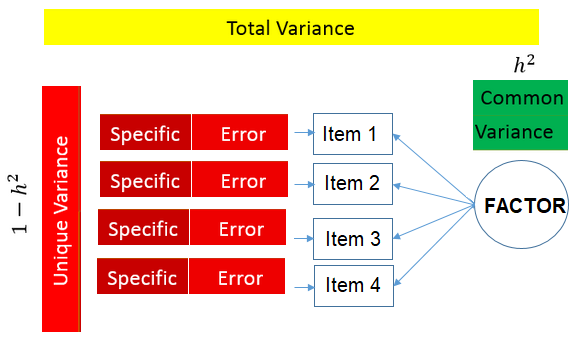
\includegraphics[width=0.75\linewidth]{figures/decompo_var} 

}

\caption[Décomposition de la variance]{Décomposition de la variance}\label{fig:decompovar}

\footnotesize


\emph{Source} : \emph{inspiré du tutoriel de l'UCLA \href{https://stats.idre.ucla.edu/spss/seminars/introduction-to-factor-analysis/a-practical-introduction-to-factor-analysis/}{ Practical Introduction to Factor Analysis: Exploratory Factor Analysis}}
\normalsize\end{figure}

L'objectif est alors de comprendre la structure des corrélations entre variables mesurées en estimant les relations entre chaque variable mesurée et les facteurs communs. Mathématiquement :
\begin{equation} 
Y = \Lambda F + \Psi E
\label{eq:eq1}
\end{equation}
Avec :
\begin{itemize}
\tightlist
\item
  \(F[n, m]\) la matrice des scores aux \(m\) facteurs communs ;
\item
  \(\Lambda [p, m]\) la matrice de saturation (en anglais \emph{loadings}) dont chaque élément représente l'influence linéaire d'un facteur commun sur une variable observée ;
\item
  \(E[n, p]\) la matrice des scores aux \(p\) facteurs uniques ;
\item
  \(\Psi [p, p]\) la matrice diagonale des variances uniques des variables observées (définies positives).
\end{itemize}
Comme le nombre de variables inconnues (les \(m\) facteurs communs et \(p\) facteurs uniques) est supérieur au nombre de variables connues (\(p\) variables observées), le modèle est indéterminé. Différentes hypothèses supplémentaires sont nécessaires pour obtenir une formule pour la matrice de corrélations \(R\) (équation \eqref{eq:eq2}) :
\begin{itemize}
\tightlist
\item
  les moyennes des facteurs communs et uniques sont nulles
\item
  les facteurs communs ne sont pas corrélés aux facteurs uniques
\item
  les facteurs uniques ne sont pas mutuellement corrélés.
\end{itemize}
L'équation fondamentale de l'AF s'écrit alors (Mulaik (2009)) :
\begin{equation} 
R = \Lambda \Phi \Lambda' + \Psi^2
\label{eq:eq2}
\end{equation}
Avec :
\begin{itemize}
\tightlist
\item
  \(R[p, n]\) la matrice de corrélation des \(p\) variables observées ;
\item
  \(\Phi [p, p]\) la matrice de corrélation entre facteurs communs.
\end{itemize}
Si l'on suppose que les facteurs communs sont orthogonaux, alors \(\Phi=I_p\) et les \(\Lambda\Lambda'\) correspondent aux communautés des variables observées et on a :
\begin{equation} 
R = \Lambda \Lambda' + \Psi^2
\label{eq:eq3}
\end{equation}
Par ailleurs, pour que le modèle soit bien déterminé, on doit avoir un nombre minimal d'indicateurs \(p\) dans notre modèle : \(p > \frac{1}{2} [ (2m + 1) + \sqrt{8m + 1} ]\) (Ledermann (1937)). C'est-à-dire au moins 3 variables pour 1 facteur, 5 variables pour 2 facteurs, 6 variables pour 3 facteurs, etc.

\hypertarget{mise-en-ux153uvre-de-lafe}{%
\subsection{Mise en œuvre de l'AFE}\label{mise-en-ux153uvre-de-lafe}}

\hypertarget{extraction-des-facteurs-communs}{%
\subsubsection{Extraction des facteurs communs}\label{extraction-des-facteurs-communs}}

Les paramètres du modèle à estimer à partir des données observées correspondent aux \(pm\) saturations des variables observées sur les \(m\) facteurs et aux \(p\) variances uniques des variables observées, soient en tout \(p(m+1)\) paramètres\footnote{Ce calcul suppose que la matrice de corrélation de la population est disponible.}.

La méthode d'extraction la plus connue est algébrique (et non statistique). Il s'agit de l'analyse en axes principaux avec estimation des communautés initiales (\emph{PAF : iterated Principal Axis Factoring}). Cette méthode est conditionnelle aux estimations a priori des communautés et est basée sur l'ACP (Hotelling (1933)) de la matrice de corrélation réduite \(R^* = R - \Psi^2\). Elle présente les avantages de ne nécessiter aucune hypothèse sur la distribution des variables observées, de pouvoir être employée quand la matrice de corrélation n'est pas régulière, de rencontrer moins de problèmes de convergence que des méthodes statistiques et de ne pas conduire à des « cas Heywood » (variances uniques négatives).

A partir des années 1960, l'accroissement de la puissance de calcul computationnel rend possible une estimation plus rigoureuse des saturations et des variances uniques. Divers algorithmes d'estimation, désormais statistiques, sont développés pour trouver les valeurs de \(\Lambda\) et de \(\Psi^2\). Ils sont techniquement complexes mais faciles à mettre en œuvre dans la pratique pour estimer les paramètres d'une AFE. En particulier, Jöreskog (1967) propose un modèle statistique aléatoire accompagné d'une procédure d'optimisation numérique permettant l'estimation du maximum de vraisemblance\footnote{L'avantage de l'estimation par maximum de vraisemblance est que cette méthode s'accompagne de nombreux indicateurs permettant de comparer la qualité de l'estimation du modèle et de mettre en place des tests de significativité et intervalles de confiance des saturations. Cette méthode repose toutefois sur une hypothèse de normalité multivariée. Pour ces raisons, il est parfois utile d'utiliser d'autres méthodes comme les principaux facteurs.} des paramètres du modèle en facteurs communs.
\begin{equation} 
y = \Lambda f + e 
\label{eq:eq4}
\end{equation}
Avec :
\begin{itemize}
\tightlist
\item
  \(y[p, 1]\) un vecteur aléatoire de \(p\) variables observées de moyenne \(\mu=0\) et de matrice de covariance \(\Sigma\) sur la population ;
\item
  \(f [m, 1]\) un vecteur aléatoire de \(m \leq p-1\) facteurs communs ;
\item
  \(\Lambda [p, m]\) une matrice des saturations des \(p\) variables observées sur les \(m\) facteurs ;
\item
  \(E[p, 1]\) un vecteur aléatoire des variances uniques des \(p\) variables observées.
\end{itemize}
Avec les hypothèses supplémentaires suivantes :
\begin{itemize}
\tightlist
\item
  \(E(f) = E(e) = E(fe') = 0\)
\item
  \(E(ee') = \Psi^2\)
\end{itemize}
Et si \(E(ff') = I_m\), alors on retrouve :
\begin{equation} 
\Sigma = \Lambda \Lambda' + \Psi^2
\label{eq:eq5}
\end{equation}
Le modèle factoriel représente maintenant l'hypothèse statistique testable que la matrice de covariance de la population a la structure impliquée par l'équation \eqref{eq:eq5} pour un nombre prescrit \(m\) de facteurs. Il s'agit alors, si l'on suppose correcte l'équation fondamentale de l'AF sur la population, de trouver les meilleures estimations au sens du maximum de vraisemblance qui minimisent la distance entre la matrice de covariance observée \(S\) et la matrice de covariance \(\hat \Sigma = \hat{\Lambda}_m \hat{\Lambda}_m' + \hat {\Psi}^2\) impliquée par le modèle en facteurs communs où \(\hat{\Lambda}_m\) et \(\hat {\Psi}^2\) sont les estimations des valeurs « vraies » de \(\Lambda_m\) et \(\Psi^2\) dans la population.

\hypertarget{la-duxe9termination-du-nombre-de-facteurs-communs}{%
\subsubsection{La détermination du nombre de facteurs communs}\label{la-duxe9termination-du-nombre-de-facteurs-communs}}

Il faut ensuite déterminer le nombre de facteurs communs nécessaires pour obtenir une matrice de saturation reconstruisant le mieux possible la matrice de corrélation entre variables observées (équation \eqref{eq:eq3}). Comme pour l'analyse en composantes principales, de nombreuses règles et procédures existent pour déterminer le nombre optimal de facteurs. Cette procédure est, en outre, ici d'autant plus importante que le nombre de facteurs choisis modifie les résultats obtenus alors que, dans une ACP, ce choix n'influe qu'au moment d'effectuer une interprétation des résultats puisqu'il est fait a posteriori. C'est pourquoi il est recommandé de s'appuyer sur plusieurs critères. En voici deux basés sur les valeurs propres de la matrice de corrélations :
\begin{enumerate}
\def\labelenumi{\arabic{enumi}.}
\item
  La règle de Kaiser-Guttman consiste à extraire un nombre de facteurs égal au nombre de valeurs propres supérieures ou égales à 1 (Guttman (1954); Kaiser (1960)).
\item
  Appliquée à la matrice de corrélation réduite, la version graphique ou numérique du scree-test de Cattell (1966) est employée pour déterminer une rupture de pente dans la courbe des valeurs propres à partir de laquelle la variance restante est jugée de faible importance ; le nombre de facteurs à extraire est alors donné par le nombre de valeurs propres supérieures à la valeur du point de rupture.
\end{enumerate}
\hypertarget{sec:annexeAFrotation}{%
\subsubsection{La rotation de la structure factorielle initiale}\label{sec:annexeAFrotation}}

La structure orthogonale initiale (équation \eqref{eq:eq4}) n'est qu'une représentation parmi une infinité de solutions factorielles qui permettent de reconstruire les corrélations du modèle étudié. C'est pourquoi cette structure initiale est habituellement transformée en appliquant une rotation -- orthogonale ou oblique -- à la matrice de saturation afin d'obtenir une structure simple plus facilement interprétable sans pour autant changer l'estimation du modèle\footnote{Alors qu'en ACP, appliquer une rotation change la solution}.

Les premières méthodes de rotation utilisées par L. Thurstone (1947) étaient géométriques. Elles étaient non seulement chronophages lorsque le nombre de facteurs (et donc de plans) étaient élevés mais on leur reprochait également d'être guidées par l'intuition des analystes et non par des hypothèses explicites.

Les méthodes analytiques de rotation qui apparurent par la suite reposent sur des principes formels indépendants du contenu des variables et visent à mieux faire apparaître les saturations élevées ou « saillantes » des variables sur les facteurs. Le modèle factoriel exploratoire le plus restreint fait l'hypothèse de corrélations nulles entre facteurs (rotation orthogonale), plusieurs variantes de ce type existent : Varimax, Quartimax, Parsimax, Orthomax. Une représentation plus plausible de la réalité et généralement recommandée est fournie par le modèle factoriel exploratoire non restreint qui fait l'hypothèse de facteurs corrélés (rotation oblique). Ses différentes variantes sont encore plus nombreuses : Quartimin, Promax, Orthoblique, Orthomin, Direct Oblimin, Geomin, Promaj, Promin, etc.

\hypertarget{sec:annexeAFAFC}{%
\section{Analyse en facteurs communs confirmatoire (AFC)}\label{sec:annexeAFAFC}}

L'Analyse en facteurs communs confirmatoire (AFC\footnote{A ne pas confondre avec l'acronyme de l'« Analyse factorielle des correspondances », une autre méthode, cette fois-ci d'analyse factorielle, non utilisée ici.} ; Jöreskog (1969) et Jöreskog (1971)) cherche comme l'AFE à reproduire les relations entre des variables observées avec un plus petit nombre de facteurs mais les deux méthodes diffèrent dans leur philosophie. Alors que l'objectif de l'AFE est de déterminer le nombre de facteurs communs, corrélés ou pas par hypothèse, et d'identifier des indicateurs notoires des facteurs parmi les variables observées (approche \emph{data-driven}), celui de l'AF confirmatoire est de tester empiriquement l'hypothèse d'une structure factorielle prédéfinie par le chercheur. Le cadre théorique doit donc être suffisamment explicite pour pouvoir incorporer des hypothèses structurales dans la spécification et l'estimation du modèle afin de tester celles-ci directement.

Il est parfois utile de mobiliser AFE et AFC dans une même recherche. En pratique, on utilise souvent une AFE avec rotation oblique avant une AFC pour voir si les hypothèses structurales théoriques que l'on formule se confirment bien empiriquement. On peut également utiliser une AFE sur une première moitié de l'échantillon pour spécifier un modèle confirmatoire que l'on estime sur la deuxième partie de l'échantillon par une AFC.

Le modèle de l'AF confirmatoire est le même que celui de l'AF exploratoire en facteurs obliques. On considère toujours \(m\) facteurs communs (dont on fixe cette fois-ci le nombre) pour lesquels il faut estimer la matrice de saturation \(\Lambda\).
\begin{equation} 
\Sigma = \Lambda \Phi \Lambda' + \Theta 
\label{eq:eq6}
\end{equation}
Avec :
\begin{itemize}
\tightlist
\item
  \(\Sigma [p, p]\) la matrice de covariance des \(p\) variables observées ;
\item
  \(\Lambda [p, m]\) la matrice creuse\footnote{On fixe à 0 les saturations des variables observées sur les facteurs dont elles ne sont pas des indicateurs. Les paramètres estimés sont dits libérés.} de saturation des \(p\) variables observées sur les \(m\) facteurs ;
\item
  \(\Phi[p, p]\) la matrice de covariance entre facteurs communs (qui peuvent ou non être corrélés) ;
\item
  \(\Theta [p, p]\) la matrice de covariance des erreurs des \(p\) variables observées\footnote{Pour rappel, dans l'expression de \(\Sigma\) en AFE, \(\Theta\) était remplacé par \(\Psi^2\) telle que \(\Psi [p, p]\) était la matrice diagonale des variances uniques des variables observées, l'AF confirmatoire accepte l'hypothèse d'erreurs corrélées, par exemple en cas d'erreurs de mesure.}.
\end{itemize}
À ces restrictions structurales, dont le bien-fondé peut être testé, s'ajoutent des contraintes d'identification du modèle qui sont nécessaires pour obtenir une solution unique. La métrique des facteurs est identifiée en imposant \(m\), par exemple en fixant une saturation par facteur à une constante non nulle (1 en général) ou en fixant à 1 les variances des facteurs comme dans l'AF exploratoire. L'indétermination de la rotation est résolue en imposant au moins \(m(m-1)\) contraintes, par exemple en libérant les éléments sous-diagonaux de \(\Phi\) et en fixant \((m-1)\) saturations à 0 par facteur. Le nombre de contraintes d'identification et de restrictions structurales est donc plus élevé dans l'AF confirmatoire que dans l'AF exploratoire (cf.~figure \ref{fig:afeafc}).
\begin{figure}[!ht]

{\centering 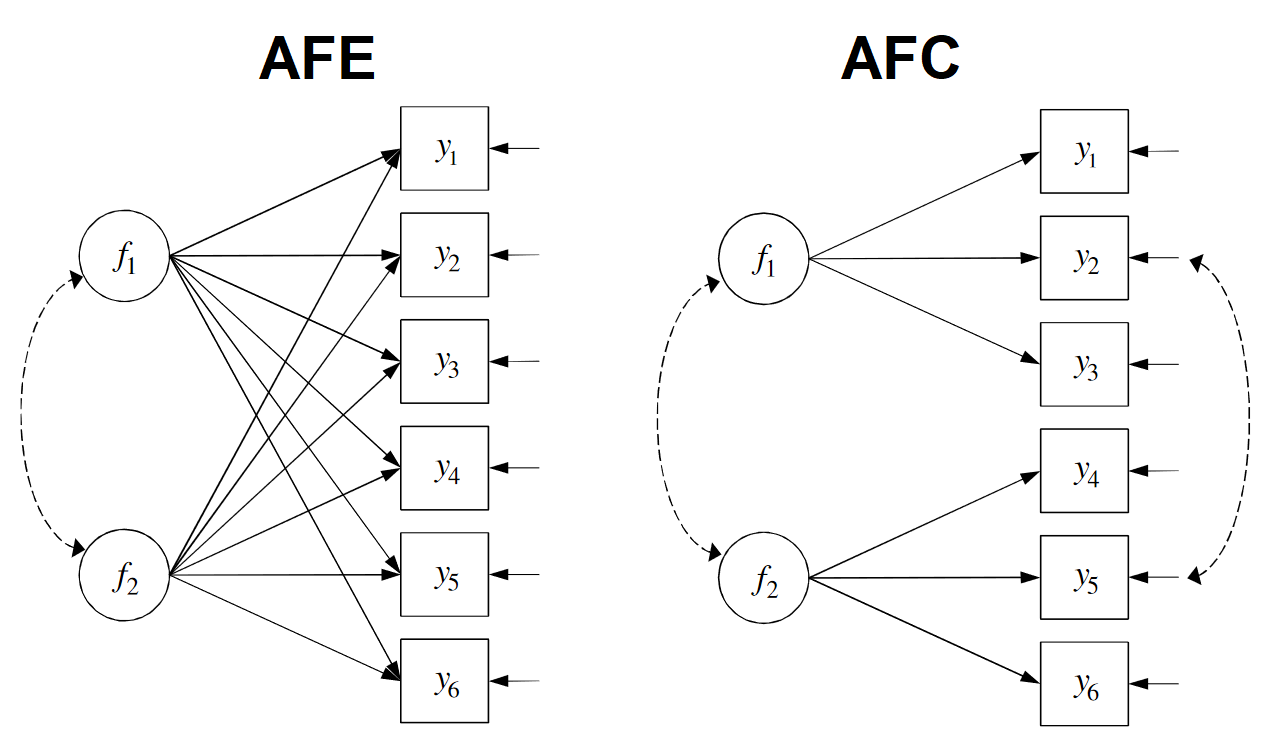
\includegraphics[width=0.75\linewidth]{figures/AFE_AFC} 

}

\caption[Analyses en facteurs communs exploratoire (AFE) et confirmatoire (AFC)]{Analyses en facteurs communs exploratoire (AFE) et confirmatoire (AFC)}\label{fig:afeafc}

\footnotesize


\emph{Source} : \emph{inspiré de Juhel (2019)}
\normalsize\end{figure}

L'AFC comporte plusieurs étapes. Il faut d'abord, comme dans l'AF exploratoire, sélectionner les variables et les individus. L'étape de spécification consiste à choisir un certain nombre de facteurs et à fixer à 0, éventuellement à contraindre à l'égalité, certains paramètres des matrices \(\Lambda\), \(\Phi\) et \(\Theta\), en s'assurant que le nombre de paramètres à estimer est inférieur ou égal au nombre de degrés de liberté du modèle, lui-même fonction du nombre d'éléments de la matrice de covariance des variables observées. Une fois ces restrictions spécifiées, le modèle est ajusté aux données en employant l'une ou l'autre des méthodes d'estimation offertes par des programmes de modélisation structurale, le plus souvent le maximum de vraisemblance (\emph{ML}), de telle sorte que la matrice de covariance impliquée par le modèle \(\hat \Sigma = \hat{\Lambda} \hat{\Phi} \hat{\Lambda}’ + \hat {\Theta}\) reproduise le mieux possible la matrice de covariance de l'échantillon.

L'étape de rotation de \(\Lambda\) est ici impossible car elle conduirait à une modification des valeurs des saturations fixées à 0 lors de la spécification du modèle.

L'ajustement du modèle est ensuite évalué au niveau global et au niveau de l'estimation de chaque paramètre. L'ajustement global est mesuré avec un test du \(\chi^2\) du rapport de vraisemblance qui conduit au rejet du modèle lorsqu'il est significatif. L'évaluation de l'ajustement global prend également appui sur divers indices d'ajustement (le \emph{Goodness-of-FIt statistic}, le \emph{Root Mean Square Error of Approximation}, le \emph{Standardised Root Mean square Residual}\ldots). Des critères d'information (par exemple l'\emph{Akaike Information Criterion}, le \emph{Bayesian Information Criterion}, le Cross-Validation index\ldots) peuvent aussi servir à comparer plusieurs alternatives plausibles du modèle.

Si l'ajustement du modèle est de bonne qualité, il est possible d'affirmer que la structure factorielle spécifiée est compatible avec les données sans pouvoir se prononcer pour autant sur l'existence d'autres modèles, non testés, également compatibles avec les données. Si l'ajustement du modèle n'est pas satisfaisant, la structure factorielle pré-spécifiée peut être rejetée avec certitude et l'analyse s'arrête dans une approche strictement confirmatoire. Mais en général, le modèle est à nouveau spécifié en fixant, contraignant à l'égalité ou libérant des paramètres sur la base d'arguments substantiels ou d'éléments empiriques comme les erreurs-types des estimations et les indices de modification (par exemple, en fixant à 0 les paramètres non statistiquement significatifs). Cette « mise à jour » du modèle est alors estimée et son ajustement évalué. Lorsque ces étapes sont répétées jusqu'à obtenir un ajustement acceptable, la différence entre l'AF exploratoire et l'AF confirmatoire s'estompe.

Ces dernières années, les modèles d'AFC ont été intégrés dans des modèles d'équations structurelles pour lesquels les facteurs sont régressés sur d'autres variables observées (« covariables externes »). Ces modèles MIMIC (\emph{multiple indicators multiple causes model} ; Jöreskog \& Goldberger (1975)) présentent l'avantage de permettre l'estimation de l'influence statistique de variables observées sur des facteurs sans avoir à calculer de scores factoriels.

\hypertarget{sec:annexeAFACM}{%
\section{Méthodes d'Analyses factorielles}\label{sec:annexeAFACM}}

\hypertarget{sec:annexeAFACMdescri}{%
\subsection{Les différentes méthodes}\label{sec:annexeAFACMdescri}}

\hypertarget{objectifs}{%
\subsubsection{Objectifs}\label{objectifs}}

Les techniques d'analyse factorielle ne supposent pas l'existence de variables latentes sous-jacentes aux variations et covariations observées et visent simplement à redistribuer la variance totale des variables observées en composantes afin d'opérer à une « réduction de données ».

Alors que l'Analyse en Composantes Principales (ACP, Hotelling (1933)) concerne des variables uniquement continues, l'Analyse Factorielle des Correspondances (Benzécri (1982)) permet d'analyser le lien entre deux variables discrètes. Concrètement, il s'agit de réaliser une ACP sur les profils lignes et colonnes du tableau de contingence en utilisant une distance du \(\chi^2\).

Enfin, l'ACM est une simple extension de l'aire d'applicabilité de l'Analyse Factorielle des Correspondances, en étendant le cas des tables de contingences à des « tableaux disjonctifs complet » (TDC) ou « tableaux de Burt » (TB) afin d'analyser plus de deux variables discrètes. Un exemple typique de ces données est celui des enquêtes d'opinion comme le Baromètre d'opinion de la Drees que nous mobilisons.

Comme pour l'ACP, l'ACM permet une représentation des individus en suivant des objectifs similaires (choix du nombre d'axes, interprétation, contribution, qualité\ldots).

\hypertarget{formalisation-mathuxe9matique-1}{%
\subsubsection{Formalisation mathématique}\label{formalisation-mathuxe9matique-1}}

Soit un TDC concernant \(I\) individus décrits par \(J\) variables qualitatives, pouvant prendre en tout \(K\) modalités. Supposons que la première variable prend les modalités\(\{1,2,...,K_{1}\}\), que la deuxième variable prend les modalités \(\{K_{1}+1,K_{1}+2,...,K_{1}+K_{2}\}\) et ainsi de suite. Soient \(K=\sum _{j}K_{j}\) et \(\{1,2,...,K\}\) les \(K\) modalités possibles. On note \(X\) ce TDC à \(I\) lignes et \(K\) colonnes dans lequel, à l'intersection de la ligne \(i\) et de la colonne \(k\) (associée à la modalité \(k\)), on trouve :
\begin{itemize}
\tightlist
\item
  1 si l'individu \(i\) possède la modalité \(k\) ;
\item
  0 sinon
\end{itemize}
Notons qu'il est possible d'inclure une variable quantitative dans l'analyse à condition de remplacer ses valeurs numériques en plage de valeur, afin de la convertir en variable catégorielle.

Le traitement mathématique du TDC \(X\) est le suivant : On calcule d'abord \(Z=X/(IK)\), puis le vecteur \(r\), qui contient la somme en ligne de la matrice \(Z\) et \(c\), qui contient la somme en colonne de la matrice \(Z\). On note également \(D_{r}={\text{diag}}(r)\) et \(D_{c}={\text{diag}}(c)\) les matrices diagonales issues de \(r\) et \(c\) respectivement. L'étape clé est une décomposition en valeurs singulières de la matrice suivante :

\[M=D_{r}^{-1/2}(Z-rc^{t})D_{c}^{-1/2}\]

La décomposition de \(M\) donne accès aux matrices \(P\), \(\Delta\) et \(Q\) telles que \(M=P\Delta Q^{t}\) avec \(P\), \(Q\) deux matrices unitaires et \(\Delta\) est la matrice diagonale généralisée contenant les valeurs singulières ordonnées de la plus grande à la plus petite. \(\Delta\) a les mêmes dimensions que \(Z\). Les coefficients diagonaux de \(\Delta ^{2}\) sont les valeurs propres de \(Z\) et correspondent à l'inertie de chacun des facteurs. Ces facteurs sont les coordonnées des individus (ligne) ou variables (colonne) sur chacun des axes factoriels. Les coordonnées des individus dans ce nouvel espace vectoriel sont données par la formule suivante :

\[F=D_{r}^{-1/2}P\Delta\]

La \(i\)-ième ligne de \(F\) contient les coordonnées du \(i\)-ième individu dans l'espace factoriel, tandis que les coordonnées des variables dans le même espace factoriel sont données par :

\[G=D_{c}^{-1/2}Q\Delta ^{t}\]

\hypertarget{sec:annexeAFACMguttman}{%
\subsection{Effet Guttman}\label{sec:annexeAFACMguttman}}

En analyse factorielle, il arrive parfois que le nuage projeté sur le premier plan factoriel ait une allure parabolique. Ce phénomène est appelé effet Guttman. Il révèle l'existence d'un premier axe associé à une valeur propre particulièrement élevée (épuisant à lui-seul une bonne partie de l'inertie totale du nuage) qui trie l'ensemble des variables selon une même échelle et signale une redondance entre les variables étudiées. Ce phénomène se présente souvent en ACM, en particulier en présence de variables au nombre de modalités impaire. L'axe principal oppose alors des situations extrêmes alors que le deuxième axe oppose les individus moyens à ces deux extrêmes.

Si cette situation se présente, il est possible (mais non assuré) de trouver du sens à l'interprétation des axes qui suivent. Lorsque l'effet Guttman est lié à la présence de modalités médianes dans les variables analysées, il est aussi possible de tenter de dichotomiser ces variables. D'autres méthodes de correction, telles que l' « analyse des correspondances dédoublée » (Benzécri, 1980) existent mais posent des difficultés d'interprétation.

Joindre les points qui représentent l'effet Guttman permet d'examiner les « accidents » de la courbe, qui représentent une répartition originale par rapport à la norme.

\hypertarget{sec:annexeAFACMcompa}{%
\subsection{Analyse Factorielle versus Analyse en facteurs communs}\label{sec:annexeAFACMcompa}}

Même s'il y a souvent assimilation entre analyse factorielle et analyse en facteurs communs, ces deux notions sont pourtant très différentes : la première correspond à un modèle descriptif des données alors que la seconde est un modèle structurel.

Les méthodes d'analyse factorielle -- ACP pour les variables quantitatives et son équivalent ACM pour les variables qualitatives -- ont pour principal objectif la réduction de la dimension des données, c'est-à-dire construire de nouvelles variables, ordonnées par importance et résumant le plus d'information possible à partir des variables initiales. Dans ces méthodes, la variance unique est considérée inexistante et la variance commune devient alors la variance totale. Chaque variable est simplement mesurée comme une fonction linéaire des composantes principales et la structure des corrélations entre variables n'est pas nécessairement conservée.

À l'inverse, l'AF différencie variances commune et unique afin de chercher à identifier des facteurs latents. Elle cherche, contrairement aux méthodes d'analyse factorielle, à comprendre la structure des corrélations (termes non diagonaux de la matrice \(\Sigma\)) entre les variables mesurées dans la base de données et ne se focalise pas sur la variance (termes diagonaux). Les facteurs construits tiennent ainsi compte de la variance commune (plutôt que totale comme dans une analyse factorielle) et la corrélation entre deux variables dépend alors de la similarité de leur relation avec les facteurs latents.

Malgré ces différences, les méthodes d'analyse factorielle peuvent toutefois dans certains cas se substituer à l'analyse en facteurs communs. De nombreux articles, comme Velicer \& Jackson (1990), indiquent même qu'il y a en pratique très peu de différences entre les deux approches dans la majeure partie des cas\footnote{Velicer \& Jackson (1990) vont même plus loin en indiquant que les différences entre méthodes se font surtout sentir quand les modèles s'estiment mal, avec des saturations très faibles et que ces différences sont souvent en défaveur de l'AF.} et que, même mathématiquement, ces méthodes sont voisines. Les méthodes d'analyse factorielle ont aussi comme gros avantage un fonctionnement computationnel simplifié car elles utilisent des méthodes d'estimation algébriques, plus simples que les méthodes types maximum de vraisemblance mobilisées en AF. Les méthodes d'AF se confrontent parfois aux « cas Heywood » (évoqués plus haut), c'est-à-dire des situations où les communautés des variables mesurées sont supérieures ou égales à 1 et faussent la modélisation (une variable ne peut pas résumer plus de 100 \% de la variance).

Mais même si ces deux approches produisent parfois des résultats similaires, ce n'est pas le cas dans de nombreux contextes : quand les données contiennent des erreurs de mesure (rendues compte dans les AF mais pas en analyse factorielle), ou des valeurs extrêmes (non supportées en analyse factorielle). Par ailleurs, les modèles en facteurs communs peuvent être testés car supposent certaines hypothèses structurelles sur les données. Le modèle est rejeté s'il est mal estimé par les données, chose qui ne peut pas être faite avec des analyses factorielles.

\backmatter

\hypertarget{bibliographie}{%
\chapter*{Bibliographie}\label{bibliographie}}
\addcontentsline{toc}{chapter}{Bibliographie}

\markboth{Bibliographie}{Bibliographie}

\noindent

\setlength{\parindent}{-0.20in}
\setlength{\leftskip}{0.20in}
\setlength{\parskip}{8pt}

\bibliography{}

\hypertarget{refs}{}
\begin{CSLReferences}{1}{0}
\leavevmode\hypertarget{ref-antunez2019franccais}{}%
Antunez, K., \& Papuchon, A. (2019). Les fran{ç}ais plus sensibles aux in{é}galit{é}s de revenus et plus attach{é}s au maintien des prestations sociales. Synth{è}se des r{é}sultats du barom{è}tre d'opinion 2018 de la drees.

\leavevmode\hypertarget{ref-argouarc2016niveaux}{}%
Argouarc'h, J., \& Boiron, A. (2016). Les niveaux de vie en 2014.

\leavevmode\hypertarget{ref-auzuret2020signifie}{}%
Auzuret, C. (2020). Que signifie sortir de la pauvret{é}? Retrieved from \url{https://laviedesidees.fr/Que-signifie-sortir-de-la-pauvrete.html}

\leavevmode\hypertarget{ref-benzecri1982histoire}{}%
Benzécri, J.-P. (1982). \emph{Histoire et pr{é}histoire de l'analyse des donn{é}es}. Dunod.

\leavevmode\hypertarget{ref-burt1941factors}{}%
Burt, C. (1941). The factors of the mind: An introduction to factor-analysis in psychology.

\leavevmode\hypertarget{ref-cahuc2014apprentissage}{}%
Cahuc, P., Ferracci, M., Tirole, J., \& Wasmer, É. (2014). L'apprentissage au service de l'emploi. \emph{Notes Du Conseil d'analyse Economique}, (9), 1--12.

\leavevmode\hypertarget{ref-calvo20192018}{}%
Calvo, M. (2019). En 2018, le nombre d'allocataires de minima sociaux repart l{é}g{è}rement {à} la hausse.

\leavevmode\hypertarget{ref-castel2014metamorphoses}{}%
Castel, R. (2014). \emph{Les m{é}tamorphoses de la question sociale: Une chronique du salariat}. Fayard.

\leavevmode\hypertarget{ref-castel2004insecurite}{}%
Castel, R., \& Beland, D. (2004). L'ins{é}curit{é} sociale: Qu'est-ce qu'{ê}tre prot{é}g{é}? \emph{The Canadian Review of Sociology}, \emph{41}(1), 88.

\leavevmode\hypertarget{ref-cattell1966scree}{}%
Cattell, R. B. (1966). The scree test for the number of factors. \emph{Multivariate Behavioral Research}, \emph{1}(2), 245--276.

\leavevmode\hypertarget{ref-cayouette2019saisir}{}%
Cayouette-Remblière, J., \& Ichou, M. (2019). Saisir la position sociale des m{é}nages: Une approche par configurations. \emph{Revue Francaise de Sociologie}, \emph{60}(3), 385--427.

\leavevmode\hypertarget{ref-cingolani2005precarite}{}%
Cingolani, P. (2005). La pr{é}carit{é}. Paris, PUF, coll.{{}} \emph{Que Sais-Je}.

\leavevmode\hypertarget{ref-dauphin2014pauvrete}{}%
Dauphin, S., \& Domingo, P. (2014). Pauvret{é} et politiques publiques: Des hommes et des femmes dans les m{ê}mes situations? \emph{Informations Sociales}, (2), 108--118.

\leavevmode\hypertarget{ref-demaison2020france}{}%
Demaison, C., Grivet, L., Lesdos, C., \& Maury-Duprey, D. (2020). France, portrait social. Edition 2020.

\leavevmode\hypertarget{ref-duvoux2018qui}{}%
Duvoux, N., \& Papuchon, A. (2018). Qui se sent pauvre en france? \emph{Revue Fran{ç}aise de Sociologie}, \emph{59}(4), 607--647.

\leavevmode\hypertarget{ref-duvoux2020insecurite}{}%
Duvoux, N., \& Papuchon, A. (2020). L'ins{é}curit{é} sociale comme condition et comme approche: {é}l{é}ments de r{é}ponse {à} lilian lahieyte et serge paugam. \emph{Revue Fran{ç}aise de Sociologie}, \emph{61}(2), 293--304.

\leavevmode\hypertarget{ref-eidelman2019renovation}{}%
Eidelman, A., \& Chardon, O. (2019). La r{é}novation de la nomenclature socioprofessionnelle (2018-2019). Retrieved from \url{http://www.epsilon.insee.fr/jspui/bitstream/1/116630/1/CNIS_rapport_2019_156.pdf}

\leavevmode\hypertarget{ref-erikson1984social}{}%
Erikson, R. (1984). Social class of men, women and families. \emph{Sociology}, \emph{18}(4), 500--514.

\leavevmode\hypertarget{ref-esping1990three}{}%
Esping-Andersen, G. (1990). \emph{The three worlds of welfare capitalism}. Princeton University Press.

\leavevmode\hypertarget{ref-fabrigar1999evaluating}{}%
Fabrigar, L. R., Wegener, D. T., MacCallum, R. C., \& Strahan, E. J. (1999). Evaluating the use of exploratory factor analysis in psychological research. \emph{Psychological Methods}, \emph{4}(3), 272.

\leavevmode\hypertarget{ref-grislain2017diminution}{}%
Grislain-Letrémy, C., \& Papuchon, A. (2017). La diminution du soutien aux transferts universels en france: Les conceptions du syst{è}me de protection sociale {é}branl{é}es par la crise de 2008? \emph{Revue Francaise Des Affaires Sociales}, (1), 205--229.

\leavevmode\hypertarget{ref-grusky2013measuring}{}%
Grusky, D. B., \& Weeden, K. A. (2013). Measuring poverty: The case for a sociological approach. In \emph{The many dimensions of poverty} (pp. 20--35). Springer.

\leavevmode\hypertarget{ref-guttman1954some}{}%
Guttman, L. (1954). Some necessary conditions for common-factor analysis. \emph{Psychometrika}, \emph{19}(2), 149--161.

\leavevmode\hypertarget{ref-hotelling1933analysis}{}%
Hotelling, H. (1933). Analysis of a complex of statistical variables into principal components. \emph{Journal of Educational Psychology}, \emph{24}(6), 417.

\leavevmode\hypertarget{ref-joreskog1967some}{}%
Jöreskog, K. G. (1967). Some contributions to maximum likelihood factor analysis. \emph{Psychometrika}, \emph{32}(4), 443--482.

\leavevmode\hypertarget{ref-joreskog1969general}{}%
Jöreskog, K. G. (1969). A general approach to confirmatory maximum likelihood factor analysis. \emph{Psychometrika}, \emph{34}(2), 183--202.

\leavevmode\hypertarget{ref-joreskog1971simultaneous}{}%
Jöreskog, K. G. (1971). Simultaneous factor analysis in several populations. \emph{Psychometrika}, \emph{36}(4), 409--426.

\leavevmode\hypertarget{ref-joreskog1975estimation}{}%
Jöreskog, K. G., \& Goldberger, A. S. (1975). Estimation of a model with multiple indicators and multiple causes of a single latent variable. \emph{Journal of the American Statistical Association}, \emph{70}(351a), 631--639.

\leavevmode\hypertarget{ref-juhel2019quelques}{}%
Juhel, J. (2019). Quelques aspects de l'{é}volution et des extensions de l'analyse factorielle en facteurs communs. \emph{Bulletin de Psychologie}, (5), 379--399.

\leavevmode\hypertarget{ref-kaiser1960application}{}%
Kaiser, H. F. (1960). The application of electronic computers to factor analysis. \emph{Educational and Psychological Measurement}, \emph{20}(1), 141--151.

\leavevmode\hypertarget{ref-lahieyte2020sociologie}{}%
Lahieyte, L. (2020). Sociologie et mesure de la pauvret{é}. \emph{Revue Francaise de Sociologie}, \emph{61}(2), 275--280.

\leavevmode\hypertarget{ref-lardeux2021sentiment}{}%
Lardeux, R., Papuchon, A., \& Pirus, C. (2021). Un sentiment de pauvreté en hausse chez les jeunes adultes fin 2020.

\leavevmode\hypertarget{ref-ledermann1937rank}{}%
Ledermann, W. (1937). On the rank of the reduced correlational matrix in multiple-factor analysis. \emph{Psychometrika}, \emph{2}(2), 85--93.

\leavevmode\hypertarget{ref-lelievre2018inegalites}{}%
Lelièvre, M., \& Rémila, N. (2018). Des in{é}galit{é}s de niveau de vie plus marqu{é}es une fois les d{é}penses pr{é}-engag{é}es prises en compte.

\leavevmode\hypertarget{ref-lollivier2005trois}{}%
Lollivier, S., \& Verger, D. (2005). Trois apports des donn{é}es longitudinales {à} l'analyse de la pauvret{é}. \emph{Economie Et Statistique}, \emph{383}(1), 245--282.

\leavevmode\hypertarget{ref-mack1985poor}{}%
Mack, J., Lansley, S., \& al. (1985). \emph{Poor britain}. G. Allen \& Unwin London.

\leavevmode\hypertarget{ref-atdquartmonde}{}%
Monde, A. Q. (2019). Les dimensions cachées de la pauvreté. \emph{Recherche Participative Internationale, Paris, OCDE}.

\leavevmode\hypertarget{ref-mulaik2009foundations}{}%
Mulaik, S. A. (2009). \emph{Foundations of factor analysis}. CRC press.

\leavevmode\hypertarget{ref-onpes}{}%
ONPES. (2015). Les budgets de référence : Une méthode d'évaluation des besoins pour une participation effective à la vie sociale. \emph{Rapport 2014-2015 de l'ONPES}.

\leavevmode\hypertarget{ref-paugam2002experience}{}%
Paugam, S. (2002). L'exp{é}rience v{é}cue de la pauvret{é}. \emph{Gallie, D., \& Paugam, S. (2002). Précarité Et Intégration Sociales}, \emph{56}.

\leavevmode\hypertarget{ref-paugam2005formes}{}%
Paugam, S. (2005). \emph{Les formes {é}l{é}mentaires de la pauvret{é}}. Presses universitaires de France Paris.

\leavevmode\hypertarget{ref-paugam2020se}{}%
Paugam, S. (2020). Se sentir pauvre. \emph{Revue Fran{ç}aise de Sociologie}, \emph{61}(2), 281--292.

\leavevmode\hypertarget{ref-paugam1991disqualification}{}%
Paugam, S., \& Schnapper, D. (1991). \emph{La disqualification sociale: Essai sur la nouvelle pauvret{é}}. Presses universitaires de France Paris.

\leavevmode\hypertarget{ref-paugam2005perception}{}%
Paugam, S., \& Selz, M. (2005). La perception de la pauvret{é} en europe depuis le milieu des ann{é}es 1970. Analyse des variations structurelles et conjoncturelles. \emph{{É}conomie Et Statistique}, \emph{383}(1), 283--305.

\leavevmode\hypertarget{ref-paugam1998soutien}{}%
Paugam, S., \& Zoyem, J.-P. (1998). Le soutien financier de la famille: Une forme essentielle de la solidarit{é}. \emph{Economie Et Statistique}, \emph{308}(1), 187--210.

\leavevmode\hypertarget{ref-ponthieux2004travailleurs}{}%
Ponthieux, S. (2004). Les travailleurs pauvres: Identification d'une cat{é}gorie. \emph{Travail, Genre Et Soci{é}t{é}s}, (1), 93--107.

\leavevmode\hypertarget{ref-rawls2020theory}{}%
Rawls, J. (2020). \emph{A theory of justice}. Harvard university press (réédition de l'ouvrage de 1971).

\leavevmode\hypertarget{ref-sen1985commodities}{}%
Sen, A. (1985). Commodities and capabilities. Lectures in economics: Theory, institutions. \emph{Policy}, \emph{7}.

\leavevmode\hypertarget{ref-simmel2011pauvres}{}%
Simmel, G. (1998). \emph{Les pauvres}. trad. de l'allemand par B. Chokrane, intro. de S. Paugam et F. Schultheis, Paris, Presses universitaires de France.

\leavevmode\hypertarget{ref-spearman1961general}{}%
Spearman, C. (1904). "General intelligence" objectively determined and measured. (Réédition de 1961).

\leavevmode\hypertarget{ref-spicker2007poverty}{}%
Spicker, P., Franzoni, J. M., Leguizamón, S. A., \& Gordon, D. (2007). \emph{Poverty: An international glossary} (Vol. 1). Zed Books.

\leavevmode\hypertarget{ref-thurstone1947multiple}{}%
Thurstone, L. (1947). Multiple factor analysis. Chicago: univer. \emph{Of Chicago Press}, \emph{1956}, 131.

\leavevmode\hypertarget{ref-thurstone1935vectors}{}%
Thurstone, L. L. (1935). The vectors of mind: Multiple-factor analysis for the isolation of primary traits.

\leavevmode\hypertarget{ref-veit1987consensual}{}%
Veit-Wilson, J. H. (1987). Consensual approaches to poverty lines and social security. \emph{Journal of Social Policy}, \emph{16}(2), 183--211.

\leavevmode\hypertarget{ref-velicer1990component}{}%
Velicer, W. F., \& Jackson, D. N. (1990). Component analysis versus common factor analysis: Some issues in selecting an appropriate procedure. \emph{Multivariate Behavioral Research}, \emph{25}(1), 1--28.

\leavevmode\hypertarget{ref-wright1991familles}{}%
Wright, R. E. (1991). Les familles monoparentales et la pauvret{é} en france. \emph{Population (French Edition)}, 1265--1267.

\end{CSLReferences}

% 4eme de couverture
% \ifthispageodd{}{\newpage\thispagestyle{empty}\null}
% Use the next command with TeX Live version ≥ 2020
%\Ifthispageodd{}{\newpage\thispagestyle{empty}\null}
\newpage
\thispagestyle{empty}
\newgeometry{top=1.5cm, bottom=1.25cm, left=2cm, right=2cm}
\fontfamily{rm}\selectfont

\lhead{}
\rhead{}
\rfoot{}
\cfoot{}
\lfoot{}

\noindent
%*****************************************************
%***** LOGO DE L'EDMH *********
%*****************************************************
% \includegraphics[height=4.5cm]{}
% \vspace{1cm}
%*****************************************************
\begin{mdframed}[linecolor=Prune,linewidth=1]
\vspace{-.25cm}
\paragraph*{Titre~:} Construire l'espace social de la pauvreté avec un Baromètre d'opinion
\begin{small}
% \vspace{-.25cm}
\paragraph*{Mots clés~:} espace social ; pauvreté ; pauvreté subjective ; ACM ; analyse en facteurs communs

% \vspace{-.25cm}
%\begin{multicols}{2}
\paragraph*{Résumé~:} En mobilisant le Baromètre d'opinion de la Drees, nous avons construit un espace social de la pauvreté mobilisant trois dimensions largement citées dans la littérature : monétaire, institutionnelle et subjective. En compléments des méthodes d'analyse factorielle et d'économétrie classiques, nous avons mobilisé des méthodes en variables latentes : analyses en facteurs communs exploratoires et confirmatoires, assez peu utilisées dans les travaux français. Ces méthodes ont pu montrer que les dimensions de la pauvreté sont non seulement théoriquement construites mais également empiriquement validées. L'étude de leurs interactions permet de décrire avec plus de précisions la nature et l'étendue des phénomènes de pauvreté en France ainsi les groupes sociaux concernés par une ou plusieurs formes de pauvreté.
%\end{multicols}
\end{small}
\end{mdframed}
% Titre anglais
% \begin{mdframed}[linecolor=Prune,linewidth=1]
% \vspace{-.25cm}
% \paragraph*{Title:} Titre anglais
% 
% \begin{small}
% \vspace{-.25cm}
% \paragraph*{Keywords:} Keywords in English.
% 
% \vspace{-.5cm}
% \begin{multicols}{2}
% \paragraph*{Abstract:} Abstract in English
% \end{multicols}
% \end{small}
% \end{mdframed}


\vfill
\fontfamily{fvs}\fontseries{m}\selectfont
\noindent\begin{tabular}{p{14cm}}
\multirow{3}{16cm}[+0mm]{\small {\color{Prune} {\bf Université Paris-Saclay}\\
{\scriptsize Espace Technologique / Immeuble Discovery}\\
{\scriptsize  Route de l’Orme aux Merisiers RD 128 / 91190 Saint-Aubin, France}}}\\\mbox{}
\end{tabular}

% Index?

\end{document}
